\documentclass[12pt, oneside, a4]{book}
\usepackage[fontsize=13pt]{scrextend}
\usepackage{times}
\usepackage{listings}
\usepackage{color} % tô màu cho code
\usepackage[utf8]{vietnam}
\usepackage{amsmath,amsthm,amssymb}
\usepackage{fancyhdr}
\usepackage[left=3.50cm, right=2.00cm, top=3.50cm, bottom=3.00cm]{geometry}\usepackage{graphicx}
\usepackage{tabularx}
\usepackage[ruled]{algorithm2e}
\usepackage{url}
\usepackage[titletoc]{appendix}
\usepackage{cases}
\usepackage{wrapfig}
\usepackage{gensymb}
%\usepackage[demo]{graphicx}
\usepackage{subfig}
\usepackage{tabularx}
\usepackage[font=small,labelfont=bf]{caption} % R
\makeindex
\renewcommand{\labelenumi}{(\roman{enumi})}
\renewcommand{\baselinestretch}{1.5}
%%
\fancyhf{}
\lhead{}
\chead{}
\rhead{}
\cfoot{\thepage}
\rfoot{}
\lfoot{}
\pagestyle{fancy}
\renewcommand{\headrulewidth}{0pt}
\renewcommand{\footrulewidth}{0pt}
%doan nay them%
\newcommand{\ora}{\overrightarrow}
\newcommand{\ra}{\rightarrow}
\newcommand{\Ra}{\Rightarrow}
\newcommand{\lra}{\longrightarrow}
\newcommand{\Lra}{\Longrightarrow}
\newcommand{\la}{\leftarrow}
\newcommand{\La}{\Leftarrow}
\newcommand{\lla}{\longleftarrow}
\newcommand{\Lla}{\Longleftarrow}
\newcommand{\map}{\longmapsto}

\newcommand{\pa}{\partial}
\newcommand{\al}{\alpha}
\newcommand{\bt}{\beta}
\newcommand{\de}{\delta}
\newcommand{\De}{\Delta}
\newcommand{\tta}{\theta}
\newcommand{\e}{\varepsilon}
\newcommand{\vp}{\varphi}
\newcommand{\na}{\nabla}
\newcommand{\sm}{\sigma}
\newcommand{\Sm}{\Sigma}
\newcommand{\gm}{\gamma}
\newcommand{\Gm}{\Gamma}
\newcommand{\Om}{\Omega}
\newcommand{\R}{\mathbb R}
\newcommand{\Q}{\mathbb Q}
\newcommand{\N}{\mathbb N}
\newcommand{\Z}{\mathbb Z}
\newcommand{\Pp}{\mathbb P}
\newcommand{\Oo}{\mathcal O}
\newcommand{\K}{\mathcal K}
\newcommand{\G}{\mathcal G}
\newcommand{\DD}{\mathcal D}
\newcommand{\XX}{\mathcal X}
\newcommand{\MM}{\mathcal M}
\newcommand{\TT}{\mathcal T}
\newcommand{\VV}{\mathcal V}
\newcommand{\WW}{\mathcal W}
\newcommand{\UU}{\mathcal U}
\newcommand{\PP}{\mathcal P}
\newcommand{\LL}{\mathcal L}
\newcommand{\BB}{\mathcal B}
\newcommand{\CC}{\mathcal C}
\newcommand{\KK}{\mathcal K}
\newcommand{\HH}{\mathcal H}
\newcommand{\QQ}{\mathcal Q}
\newcommand{\cbe}{\scriptsize}
\newcommand{\On}{\widetilde{\mathcal{O}}}
\newcommand{\Mn}{\widetilde{M}}
\newcommand{\sumh}{\overline{\sum}}
\newcommand{\cho}[2]{\ensuremath{#1\choose#2}}
\newcommand{\ve}[1]{{\bf #1}}
\newcommand{\wt}[1]{\widetilde #1}
\newcommand{\norm}[1]{\left\lVert#1\right\rVert}

\newtheorem{Defi}{Definition}
\newtheorem{Not}{Notation}
\newtheorem{Lem}{Lemma}
\newtheorem{Hypo}{Hypothesis}
\newtheorem{Theo}{Theorem}
\newtheorem{Prop}{Proposition}
\newtheorem{Coro}{Corollary}
%\newtheorem{Algo}{Algorithm}
\newtheorem{Rem}{Remark}

\usepackage{cite}
\usepackage{array}

%% Đoạn này thêm
\definecolor{dkgreen}{rgb}{0,0.6,0}
\definecolor{gray}{rgb}{0.5,0.5,0.5}
\definecolor{mauve}{rgb}{0.58,0,0.82}
 
\lstset{frame=tb,
  language=C++,
  aboveskip=3mm,
  belowskip=3mm,
  showstringspaces=false,
  columns=flexible,
  basicstyle={\small\ttfamily},
  numbers=none,
  numberstyle=\tiny\color{gray},
  keywordstyle=\color{blue},
  commentstyle=\color{dkgreen},
  stringstyle=\color{mauve},
  breaklines=true,
  breakatwhitespace=true,
  tabsize=3
}
%% Kết thúc đoạn thêm

\begin{document}

\addcontentsline{toc}{chapter}{{\bf Lời nói đầu}}
%
\chapter*{Lời nói đầu}
Từ trước đến nay việc thu thập thông tin của con người thông qua việc quan sát xảy ra rất thường xuyên. Và ngày càng ra đời nhiều công cụ trợ giúp con người trong quá trình quan sát và ghi lại thông tin như máy chụp ảnh, camera,.... Đầu ra của các thiết bị này là ảnh hay video. Một nhu cầu cần thiết là trích rút thông tin từ các ảnh hay video này. Một trong các công việc quan trọng trong quá trình trích rút thông tin là thực hiện phân vùng trên các ảnh hay video này. Công việc này giúp giải quyết các vấn đề mà đôi khi không thể dùng mắt thường để quan sát được. Vì vậy đồ án này em lựa chọn đề tài "Một số phương pháp phân vùng dựa trên biên động và ứng dụng".  Đồ án thực hiện tìm hiểu một số phương pháp phân vùng và dùng tập trung vào phương pháp sử dụng biên động. Đồng thời đưa ra một mô hình cải tiến dựa trên các mô hình dựa trên biên động đã có và áp dụng mô hình cải tiến này trong phân vùng ảnh 3 chiều và  theo vết đối tượng trong video. Nội dung đồ án bao gồm  các phần sau:
\begin{itemize}
\item[i] Chương 1: Trình bày các kiến thức cơ bản về xử lý ảnh và các vấn đề trong xử lý ảnh.
\item[ii] Chương 2: Trình bày một số hướng tiếp cận cho quá trình phân vùng ảnh.
\item[iii] Chương 3: Trình bày một số mô hình phân vùng dựa trên biên động và đưa ra mô hình cải tiến.
\item[iv] Chương 4: Áp dụng mô hình cải tiến trong theo vết đối tượng trong video.
\item[v] Chương 5: Áp dụng mô hình cải tiến trong phân vùng 3 chiều.
\end{itemize}
 Em xin gửi lời cảm ơn chân thành  tới {\bf TS. Thiều Quang Tùng} đã luôn tận tình hướng dẫn, giúp đỡ để em có thể hoàn thành đồ án này.\\
Trong quá trình hoàn thiện nhưng đồ án vẫn không thể tránh khỏi những sai sót. Em rất mong nhận được những góp ý quý báu của thầy cô và các bạn để nội dung đồ án được hoàn thiện hơn nữa.\\\\
Em xin chân thành cảm ơn!\\


\begin{flushright}
Hà Nội, ngày 28 tháng 5 năm 2017\\[0.5cm]
{Sinh viên thực hiện \hspace*{1.4cm}.}\\[0.1cm]
\textbf{Đoàn Tú Anh\hspace*{2.0cm}}
\end{flushright}
\tableofcontents
\newpage
\listoffigures
\newpage
%\listoftables
\newpage

\chapter{Xử lý ảnh và các vấn đề cơ bản của xử lý ảnh}
\section{Xử lý ảnh là gì?}
Một ảnh có thể được đại diện bởi một hàm 2 chiều $f(x,y)$.Với $(x, y)$ là tọa độ của các điểm trong mặt phẳng, giá trị $f$ tại các cặp tọa độ $(x,y)$ được gọi là cường độ  hay mức xám của ảnh tại điểm đó. Ảnh số là tâp hợp hữu hạn các  phần tử, mỗi phần tử có một tọa độ riêng và một giá trị $f$ riêng. Các giá trị này gọi là $pixel$ hay $ image elements$ . Một trong các ứng dụng của ảnh số là trong ngành công nghiệp báo chí, khi ảnh lần đầu tiên được truyền qua cáp biến giữa London và NewYork. Việc truyền ảnh qua cáp biển này đã rút ngắn quá trình truyền ảnh qua Đại Tây Dương từ hơn một tuần xuống còn chưa đến 3 giờ. Một máy in đặc biệt mã hóa bức ảnh để truyền tải đi và khôi phục lại ảnh gốc ở đầu cuối. Sự phát triển của phần cứng máy tính đã giúp cho lĩnh vực đồ họa và xử lý ảnh phát triển một cách mạnh mẽ và ngày càng có nhiều ứng dụng trong cuộc sống.
\begin{center}
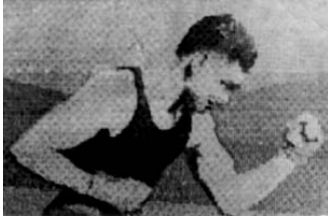
\includegraphics[]{figure/1921.png}
\captionof{figure}{Một bức ảnh được tạo ra bởi máy điện ấn năm 1921}
\end{center}

Quá trình xử lý ảnh được xem là quá trình thao tác với ảnh đầu vào để đưa ra một kết quả mong muốn. Quá trình xử lý ảnh có thể được mô tả theo sơ đồ sau:
\begin{center}
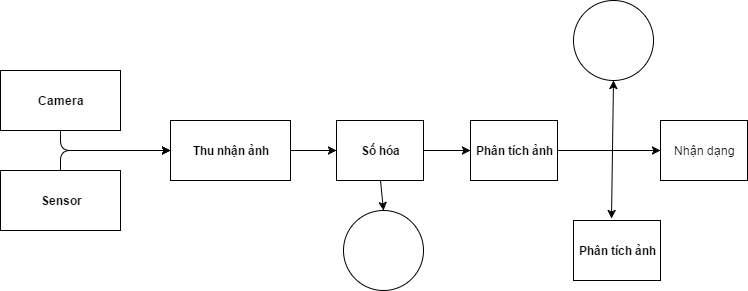
\includegraphics[scale=0.5]{figure/quatrinh.png}
\captionof{figure}{Các quá trình của xử lý ảnh}
\end{center}
Đầu tiên là quá trình thu nhận ảnh. Ảnh có thể được thu nhận qua camera. Đầu ra có thể là dạng tín hiệu tương tự hoặc cũng có thể là tín hiệu số hóa. Ngoài ra ảnh còn có thể được thu nhận qua bộ cảm ứng sensor , tranh, ảnh được quét thông qua máy quét.
Quá trình số hóa thực hiện biến đổi tín hiệu tương tự thành tín hiệu rời rạc sau đó được đưa vào quá trình phân tích, xử lý hoặc thực hiện lưu trữ ảnh.

Quá trình phân tích ảnh bao gồm nhiều bước nhỏ. Với một số ảnh, do thiết bị thu nhận ảnh, nguồn sáng hay nhiễu mà ảnh có thể bị suy biến. Do vậy chúng ta cần thực hiện quá trình tăng cường ảnh nhằm tăng chất lương hoặc làm nổi bật một số đặc tính chính của ảnh. Tiếp theo là quá tình phát hiện các đặc tính như biên ảnh (Edge Detection), phân vùng ảnh (Segmentation)...
Cuối cùng tùy theo ứng dụng mà có thể thực hiện quá trình nhận dạng, phân lớp hay ra quyết định.
 
Một hệ sử lý ảnh có thể được mô tả gồm các thành phần như hình 1.3
\begin{center}
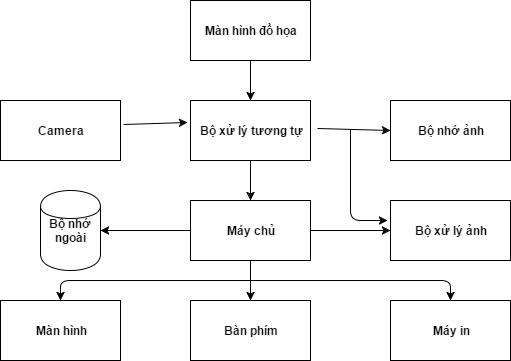
\includegraphics[scale=0.7]{figure/hethong.png}
\captionof{figure}{Các thành phần chính của hệ thống xử lý ảnh}
\end{center}
\section{Một số vấn đề trong xử lý ảnh}
\subsection{Một số khái niệm trong xử lý ảnh}
\begin{itemize}
\item Điểm ảnh: là một phần tử nhỏ nhất của ảnh. Một điểm ảnh có thể coi như gồm hai thành phần tọa độ và cường độ sáng tại một điểm trong không gian của đối tượng. 
\item Mức xám, màu: là kết quả của sự mã hóa cường độ sáng của một điểm ảnh với một giá trị số.
\end{itemize}
\subsection{Tăng cường khôi phục ảnh}
Tăng cường và khôi phục ảnh là hai quá trình có mục đích khác nhau. Tăng cường ảnh bao gồm các thao tác nhằm làm hoàn thiện trạng thái quan sát của một ảnh như: tăng cường độ tương phản, khử nhiễu. Trong khi đó khôi phục ảnh nhằm khôi phục ảnh  gần với ảnh thực nhất do nó bị biến dạng do nhiều nguyên nhân khác nhau.

Việc khôi phục ảnh nhằm tối thiểu hóa ảnh hưởng của các yếu tố môi trường bên ngoài và các hệ thống thu nhận và lưu trữ ảnh. Quá trình khôi phục ảnh có thể coi là quá trình xây dựng mô hình toán học cho các ảnh hưởng sau đó dùng ánh xạ ngược để xác định lại ảnh 
\subsection{Biến đổi ảnh}
Trong xử lý ảnh, một số trường hợp có phức tạp tính toán cao hoăc là số lượng điểm ảnh lớn. Việc dùng các phương pháp thông thường trở nên không khả thi. Vì vậy người ta thực hiện xây dựng một không gian khác đơn giản hơn và thực hiện bước chuyển đổi từ không gian gốc sang không gian này để dễ tính toán hơn. Sau khi thực hiện xử lý trên không gian mới xong, dùng phép biến đổi ngược để đưa về miền xác định ban đầu. Một số biến đổi thường được hay dùng là:
\begin{itemize}
\item Biến đổi Fourier, Sin,  Cosin
\item Biên đổi bằng tích chập, tích Kronecker
\item Các biến đổi như Kahumen Loeve, Hadamard
\end{itemize}
Ngoài ra người ta còn sử dụng một số công cụ thống kê trong biến đổi ảnh.
\subsection{Phân tích ảnh}
Việc phân tích ảnh nhằm đưa ra các mô tả đặc trưng về ảnh. Các kỹ thuật được xử dụng ở bước này nhằm xác định biên của ảnh. Ngoài ra người ta cũng sử dụng các kỹ thuật để phân vùng ảnh. Các kỹ thuật thường hay dùng là tách, hợp thành phần dựa theo các tiêu chuẩn đánh giá như màu sắc, cường độ ,... Các phương pháp thường được dùng như phân tích cây tứ phân, phân vùng dựa theo cấu trúc, phân vùng dựa theo đồ thị.
\subsection{Nhận dạng ảnh}
Nhận dạng là quá trình phân loại các đối tượng được biểu diễn theo một mô hình nào đó và gán cho chúng vào các lớp dựa theo các quy luật. Quá trình nhận dạng theo các mẫu có trước được gọi là học có thầy (supervised learning), trong trường hợp ngược lại gọi là học không có thầy(unsupervised learning). Một số cách tiếp cận khác trong nhận dạng ảnh như: 
\begin{itemize}
\item Nhận dạng dựa vào phân hoạch không gian
\item Nhận dạng  cấu trúc
\item Nhận dạng theo mạng nơron
\end{itemize}
Với hai cách tiếp cận đầu, sau khi thu nhận, ảnh cần trải qua các bước tiền xử lý làm tăng chất lượng và làm nổi bật các chi tiết, sau đó là quá trình biễu diễn và trích chọn các đặc trưng, cuối cùng mới là quá trình nhận dạng.

Trong thực tế, người ta đã áp dụng thành công nhận dạng cho nhiều đối tượng khác nhau như: 

\begin{itemize}
\item Nhận dạng vân tay phục vụ cho mục đích bảo mật và phát hiện tội phạm.
\item Nhận dạng chữ in phục vụ  cho quá trình số hóa tài liệu, tự động đọc tài liệu.
\item Nhận dạng chữ viết tay với các ràng buộc về cách viết, kiểu chữ... 
\end{itemize}
\subsection{Nén ảnh}
Việc truyền ảnh qua mạng là một thao tác được dùng thường xuyên, trong khi lượng thông tin dùng để biểu diễn ảnh lại là khá lớn. Do vậy việc nén ảnh để giảm lượng thông tin truyền đi là một nhu cầu cần thiết.

Nén ảnh là kỹ thuật lợi dụng sự dư thừa thông tin của ảnh nhằm biến đổi dữ liệu ảnh thành dạng từ mã. Mỗi phương pháp nén ảnh dựa trên các định nghĩa dư thừa khác nhau. Các định nghĩa dư thừa hay được dùng như: sự phân bố mức xám, sự lặp lại mức xám, những mẫu sử dụng tần suất cao hoặc độ dư thừa vị trí. Tùy vào thuật toán và loại ảnh mà ta có tỷ lệ nén khác nhau: 
\begin{equation*}
\textrm{Tỷ lệ nén} =\dfrac{\textrm{Dữ liệu sau nén}}{\textrm{Dữ liệu trước khi nén}}
\end{equation*}
Dựa theo các cách phân loại khác nhau người ta có các phương pháp nén ảnh khác nhau:
\begin{itemize}
\item Phân loại theo lý thuyết nén
\begin{itemize}
\item Nén không mất mát thông tin
\item Nén mất mát thông tin
\end{itemize}
\item Phân loại dựa theo cách thức thực hiện nén: 
\begin{itemize}
\item Phương pháp không gian
\item Phương pháp dựa trên  biến đổi
\end{itemize}
\item Phân loại dựa trên phương pháp mã hóa:
\begin{itemize}
\item Phương pháp nén thế hệ thứ nhất
\item Phương pháp nén thế hệ thứ hai
\end{itemize}
\end{itemize}
%\subsection{Thu nhận ảnh và các thiết bị thu nhận, biểu diễn ảnh}
%Hầu hết các ảnh chúng ta quan tâm ngày nay được tạo ra nhờ sự tổng hợp các yếu tố như : nguồn sáng, và sự phản xạ hấp thụ của các phần tử trong khung nhìn của ảnh. Các thiết bị thu nhận ảnh thông thường bao gồm máy quay (camera) cộng với bộ chuyển đổi tương tự số hoặc máy quét (scanner). Các thiết bị này có thể cho màu đen trắng hoặc ảnh màu. Với ảnh đen trắng, mức xám có thể nằm trong khoảng từ 0 đến 1. Với ảnh đa cấp xám, mức xám sẽ nằm trong khoảng từ 0 đến 255. Với ảnh màu, mỗi điểm ảnh được lưu trữ trong 3 byte vì vậy ta có khoảng $2^{8*3}=2^24$ màu. 
%
%Thiết bị ra ảnh có thể là máy in đen trắng, máy in màu hay máy vẽ (ploter). 
%Các hệ thống thu nhận ảnh thực hiện 2 quá trình:
\chapter{Một số phương pháp tiếp cận phân vùng ảnh}
Phân vùng ảnh là một bước quan trọng trong xử lý ảnh, quá trình này nhằm phân tích ảnh thành các thành phần có cùng tính chất nào đó dựa theo biên hay các vùng liên thông. Vùng ảnh là tập hợp các điểm ảnh có cùng hay gần cùng một đặc điểm nào đó. Ví dụ như mức xám, mức màu, ...  Đường bao quanh vùng ảnh được gọi là biên ảnh.
\section{Phân vùng ảnh theo ngưỡng biên độ}
Một ảnh được đặc trưng bởi các tính chất như: mức xám, độ tương phản, màu sắc,.... Ta có thể dùng ngưỡng biên độ với các đặc trưng trên để phân đoạn ảnh trong trường hợp ngưỡng biên độ đủ lớn đặc trưng cho ảnh. Kỹ thuật phân ngưỡng theo biên độ có lợi thế với ảnh nhị phân như bản in, đồ họa, ảnh màu.

Việc chọn ngưỡng sẽ bao gồm các bước sau:
\begin{itemize}
\item Xác định các đỉnh và khe của ảnh dựa vào việc phân tích lược đồ xám. Các khe có thể dùng để chọn ngưỡng
\item Chọn ngưỡng t sao cho một phần xác định trước của toàn bộ mẫu là thấp hơn t
\item Điều chỉnh ngưỡng dựa trên lược đồ xám của các điểm lân cận
\item Chọn ngưỡng theo lược đồ xám của các điểm thỏa mãn tiêu chuẩn chọn
\item Khi có mô hình phân lớp xác suất, ta thực hiện xác định ngưỡng dựa vào tiêu chuẩn xác suất nhằm cực tiểu hóa xác suất sai
\item Ta có ví dụ minh họa cho việc phân vùng dựa trên ngưỡng như sau:
\begin{center}
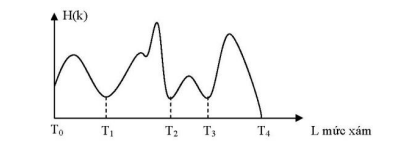
\includegraphics[]{figure/nguongbiendo.png}
\captionof{figure}{Ví dụ minh họa cách chọn ngưỡng}
\end{center}
Ở đây 5 ngưỡng được chọn và ảnh sẽ được phân vùng thành 4 vùng. Ta ký hiệu các vùng đó là $C_k$ trong đó $k=1,2,3,4$   . Các vùng sẽ được phân như sau:
\begin{equation}
P(m,n) \in C_{k}\textrm{ nếu } T_{k-1}<P(m,n)<T_{k}; k=1,2,3,4
\end{equation} 
\end{itemize}
Nếu sau khi phân vùng theo ngưỡng vừa mà chọn ảnh rõ nét thì kết thúc, ngược lại phải điều chỉnh ngưỡng và phân vùng lại cho đến khi đạt được kết quả mong muốn.
\section{Phân vùng ảnh theo miền đồng nhất}
Kỹ thuật này sử dụng tính chất đồng nhất của các đặc trưng nào đó của ảnh. Cách thức phân vùng sẽ phụ thuộc vào việc lựa chọn đặc trưng dùng để thực hiện phân vùng. Các đặc trưng thường được dùng là mức xám với ảnh đen trắng và màu với ảnh màu. Với cách tiếp cận này, các phương pháp thường được sử dụng là :
\begin{itemize}
\item  Phương pháp tách cây tứ phân
\item Phương pháp cục bộ
\item Phương pháp tổng hợp
\end{itemize}
\subsection{Phương pháp tách cây tứ phân}
Một tiêu chuẩn đồng nhất sẽ được chọn. Quá trình phân vùng sẽ thực hiện như sau: Đầu tiên ta thực hiện kiểm tra tính chất đồng nhất trên toàn bộ miền ảnh. Nếu tính đồng nhất thỏa mãn thì kết thúc thuật toán. Ngược lại miền ảnh sẽ được chia làm 4 miền con. Tiếp tục kiểm tra tính chất đồng nhất của các miền con và thực hiện phân tách khi tính chất đồng nhất không thỏa mãn. Quá trình kết thúc khi tất cả các miền con trong miền ảnh ban đầu thỏa mãn tính đồng nhất.

Phương pháp này được mô tả như sau:
\begin{lstlisting}
Func Phanvung(MienAnh)
{
dsmiencon.Push(MienAnh)
	while(dsmiencon.Count()!=0)
	{
	miendangxet=dsmiencon.Pop();
	if(!ktdongnhat(miendangxet))
		{
			m1,m2,m3,m4=miendangxet.chiamien();
			for(int i=0;i<4;i++)
			{
			dsmiencon.Push(m_i)
			}
		}
	}
}
\end{lstlisting}

Tiêu chuẩn đồng nhất có thể dựa vào mức xám. Một cách đơn giản ta có thể chọn giá trị chênh lệch giữa giá trị mức xám lớn nhất và giá trị mức xám nhỏ nhất trong miền đang xét. Hàm kiểm tra mức xám có thể được viết như sau: Giả sử $(m_1,n_1), (m_2,n_2)$ là tọa độ điểm đầu và điểm cuối của miền đang xét
\begin{lstlisting}
Func ktdongnhat(miendangxet)
{
int min=0;
int max=255
for(i=n1;i<n_2;i++)
for(j=m1;j<m_2;j++)
	{
		if(I(i,j)<min)
		I(i,j)=min;
		if(I(i,j)>max)
		I(i,j)=max;
	}
	if((max-min)<nguong) return 1;
	return 0;
}
\end{lstlisting}
\subsection{Phân vùng ảnh dựa vào phát triển vùng cục bộ}
Ý tưởng của phương pháp này ngược lại với phương pháp cây tứ phân. Phương pháp thực hiện xét từ các miền ảnh nhỏ nhất của ảnh rồi nối chúng lại nếu chúng thỏa mãn điều kiện đồng nhất. Thực hiện tiếp tục khi không thể tiếp tục nối các miền lại với nhau nữa.
Trong cách này, hai vùng sẽ được nối lại với nhau nếu chúng thỏa mãn 2 điều kiện :
\begin{itemize}
\item Kế cận nhau
\item Có mức xám đồng nhất
\end{itemize}

Để xác định tính kế cần giữa 2 vùng người ta sử dụng tính liên thông. Có 2 quan niệm về liên thông là 4 liên thông và 8 liên thông. Với 4 liên thông,  một điểm ảnh sẽ có 4 điểm ảnh kế cận theo 2 hướng $x,y$. Còn với 8 liên thông, một điểm ảnh sẽ có 4 điểm ảnh theo 2 hướng $x,y$ là 4 điểm ảnh theo các hướng chéo $45$ độ.
\begin{center}
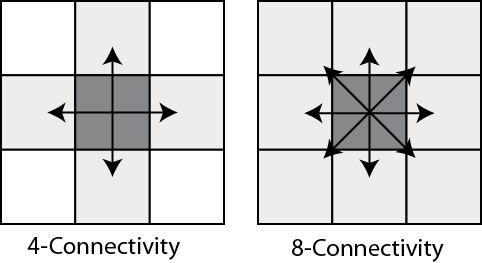
\includegraphics[scale=0.7]{figure/4-8-connectivity.png}
\captionof{figure}{4 liên thông và 8 liên thông}
\end{center}
\subsection{Phân vùng ảnh dựa trên hợp và tách vùng}
Đề khắc phục được nhược điểm của 2 phương pháp cây tứ phân và phương pháp phát triển cục bộ người ta đưa ra phương pháp kết hợp ý tưởng hợp và tách vùng của 2 phương pháp trên. Với phương pháp tách, việc thực hiện chia quá chi tiết còn với phương pháp hợp mặc dù giảm được tối thiểu số vùng sau khi chia tuy nhiên không cho ta thấy rõ được mối liên hệ giữa các miền vùng.

Phương pháp kết hợp giữa hợp và tách thực hiện như sau. Đầu tiên , ta thực hiện tách miền ảnh theo cây tứ phân, thực hiện phân đoạn từ gốc đến lá, tiếp theo tiến hành duyệt cây theo chiều ngược lại để hợp các vùng đồng nhất. Trong thao tác hợp các vùng đồng nhất, có thể có nhiều vùng thỏa mãn điều kiện đồng nhất. Vì vậy ta phải xây dựng một hàm đánh giá giá trị đồng nhất của các vùng với nhau trả về các giá trị trong đoạn $[0,1]$ trong  đó 0 là không đồng nhất, và 1 là hoàn toàn đồng nhất. Với hàm đánh giá kiểu này,  trong quá trình thực hiện thao tác hợp, trong trường hợp có nhiều vùng thỏa mãn điều kiện đồng nhất, ta sẽ thực hiện chọn vùng mà giá trị hàm đồng nhất trả về lớn nhất để thực hiện hợp vùng.
\section{Phân vùng ảnh dựa theo phát hiện biên}
Với một ảnh thì biên là một đặc tính quan trọng phục vụ làm đầu vào cho nhiều công việc khác nhau trong việc xử lý ảnh. 
Các quá trình thực hiện phân vùng theo đường biên sẽ thực hiện theo các bước như sau:
\begin{itemize}
\item Phát hiện biên
\item Làm mảnh biên
\item Nhị phân hóa đường biên
\item Biểu diễn đường biên
\item Phân vùng từ đường biên nhận được.
\end{itemize}
\subsection{Phát hiện biên }
Về cơ bản phương pháp phát hiện biên có thể chia thành hai loại chính là :
\begin{itemize}
\item Phát hiện biên trực tiếp: phương pháp này làm nổi bật biên dựa trên sự thay đổi về độ xám của các điểm ảnh. Kỹ thuật hay được dùng là đạo hàm. Trong trường hợp đạo hàm dùng là bậc nhất thì ta có phương pháp gradient, trong trường hợp đạo hàm được dùng là bậc hai thì ta có kỹ thuật laplace. Ngoài ra người ta còn sử dụng kỹ thuật đi theo đường bao dựa vào quy hoạch động.
\item Phát hiện biên gián tiếp:  Phương pháp này lợi dụng kết quả của việc phân vùng ảnh để thực hiện tìm biên. Sau khi có kết quả phân vùng ảnh thành các vùng khác nhau thì ranh giới giữa các vùng sẽ được chọn làm biên. Hai bài toán phân vùng  và bài toán tìm biên có thể xem là bài toán đỗi ngẫu. Có được đường biên ta có thể phân ảnh ra các vùng khác nhau và ngược lại có được các vùng khác nhau ta cũng có thể xây dựng đường biên từ đó. Do phần này trình bày việc áp dụng tìm biên trong việc phân vùng nên chỉ đề cập đến các phương pháp tìm biên trực tiếp.
\end{itemize}
\subsubsection{Phương pháp gradient}
Như đã đề cận ở trên, phương pháp phát hiện biên trực tiếp sử dụng sự biến thiên của cường độ ảnh. Vector gradient thể hiện tốc độ biến đối của cường độ ảnh theo các trục $x,y$ 
\begin{equation*}
\begin{cases}
 \dfrac{\partial f(x,y)}{\partial x}=f_x\approx\dfrac{f(x+dx,y)-f(x,y)}{dx}\\
 \dfrac{\partial f(x,y)}{\partial y}=f_x\approx\dfrac{f(x,y+dy)-f(x,y)}{dy}\\
   \end{cases}
\end{equation*}
Thực ra các điểm ảnh được định nghĩa một cách rời rạc nên không tồn tại đạo hàm mà thực chất đạo hàm chỉ là một mô phỏng về mặt lý thuyết và được tính xấp xỉ trong quá trình xử lý nhờ phép cuộn với một mặt lạ được định nghĩa trước:
\begin{itemize}
\item Kỹ thuật prewitt:
Kỹ thuật này sử dụng hai mặt nạ theo các hướng x,y 
\begin{align*}
   H_x= \begin{pmatrix}
        -1 & 0 & 1 \\
        -1 & 0 & 1  \\
        -1 & 0 & 1
    \end{pmatrix}
\end{align*}
\begin{align*}
   H_y= \begin{pmatrix}
        -1 & -1 & -1 \\
        0 & 0 & 0  \\
        1 & 1 & 1
    \end{pmatrix}
\end{align*}
Đạo hàm sẽ được xấp xỉ thành $I\ast H_x+I\ast H_y$

\item Kỹ thuật Sobel:
Tương tự như kỹ thuật prewitt, kỹ thuật Sobel sử dụng hai mặt nạ nhân theo hai hướng x,y
\begin{align*}
   H_x= \begin{pmatrix}
        -1 & 0 & 1 \\
        -2 & 0 & 2  \\
        -1 & 0 & 1
    \end{pmatrix}
\end{align*}
\begin{align*}
   H_y= \begin{pmatrix}
        -1 & -2 & -1 \\
        0 & 0 & 0  \\
        1 & 1 & 1
    \end{pmatrix}
\end{align*}
Đạo hàm sẽ được xấp xỉ thành $I\ast H_x+I\ast H_y$
\item Kỹ thuật Kỹ thuật la bàn: 
Kỹ thuật này sử dụng 8 mặt nạ theo 8 hướng : 0\degree, 45\degree, 90\degree, 135\degree, 180\degree, 225\degree, 270\degree, 315\degree
\begin{align*}
    \begin{matrix}
       H_1= \begin{pmatrix}
        5 & 5 & -3 \\
        5 & 0 & -3  \\
        -3 & -3 & -3
    \end{pmatrix} & H_2=\begin{pmatrix}
        5 & 5 & 5 \\
        -3 & 0 & -3  \\
        -3 & -3 & -3
    \end{pmatrix} \\
        H_3=\begin{pmatrix}
        -3 & 5 & 5 \\
        -3 & 0 & 5  \\
        -3 & -3 & -3
    \end{pmatrix} & H_4=\begin{pmatrix}
        -3 & -3 & 5 \\
        -3 & 0 & 5  \\
        -3 & -3 & 5
    \end{pmatrix}\\
       H_5= \begin{pmatrix}
        -3 & -3 & -3 \\
        -3 & 0 & 5  \\
        -3 & 5 & 5
    \end{pmatrix} & H_5=\begin{pmatrix}
        -3 & -3 & -3 \\
        -3 & 0 & -3  \\
        5 & 5 & 5
    \end{pmatrix}\\
        H_7=\begin{pmatrix}
        -3 & -3 & -3 \\
        5 & 0 & -3  \\
        5 & 5 & -3
    \end{pmatrix} & H_8=\begin{pmatrix}
        5 & -3 & -3 \\
        5 & 0 & -3  \\
        5 & -3 & -3
    \end{pmatrix}
    \end{matrix}
\end{align*}
\end{itemize}
Đạo hà sẽ được xấp xỉ thành $$\sum_{i=1}^{8} I\ast H_i$$
\subsubsection{Kỹ thuật phát hiện biên Laplace }
Trong trường hợp độ chênh lệch mức xám lớn thì phương pháp gradient hoạt động tương đối tốt. Tuy nhiên trong trường hợp độ chênh lệch mức xám thấp, phương pháp Laplace lại tỏ ra hiệu quả hơn. Thực nghiệm cho thấy toán tử Laplace nhạy cảm với nhiễu và không hỗ trợ xác định hướng của biên. Toán tử Laplace sẽ được sử dụng để xác định một điểm nằm ở vùng tối hay vùng sáng của biên. Toán tử laplace được định nghĩa như sau:

\begin{equation*}
\nabla ^2 f=\dfrac{\partial^2 f }{\partial x^2}+\dfrac{\partial^2 f }{\partial y^2}
\end{equation*}
Với 
\begin{equation*}
\begin{split}
\dfrac{\partial^2 f }{\partial x^2} &=\dfrac{\partial}{\partial x}(\dfrac{\partial f}{\partial x})\\
&\approx \dfrac{\partial f}{\partial x} (f(x+1,y)-f(x,y))\\
&\approx (f(x+1,y)-f(x,y))-(f(x,y)-f(x-1,y))\\
&\approx f(x+1,y)-2f(x,y)+f(x-1,y)
\end{split}
\end{equation*} 
và  
\begin{equation*}
\begin{split}
\dfrac{\partial^2 f }{\partial y^2} &=\dfrac{\partial}{\partial y}(\dfrac{\partial f}{\partial y})\\
&\approx \dfrac{\partial f}{\partial y} (f(x,y+1)-f(x,y))\\
& \approx (f(x,y+1)-f(x,y))-(f(x,y)-f(x,y-1)) \\
& \approx f(x,y+1)-2f(x,y)+f(x,y-1)
\end{split}
\end{equation*} 
 Do đó $\nabla ^2 f\approx f(x+1,y)+f(x,y+1)-4f(x,y)+f(x-1,y)+f(x,y-1)$
 Từ đó ta có thể xấp xỉ đạo hàm bậc 2 Laplace sử dụng ma trận 
\begin{align*}
   H_x= \begin{pmatrix}
        0 & 1 & 0 \\
        1 & -4 & 1  \\
        0 & 1 & 0
    \end{pmatrix}
\end{align*}
 Ngoài ra người ta còn sử dụng thêm các loại mặt nạ khác để xấp xỉ toán tử đạo hàm như :
 \begin{align*}
    \begin{matrix}
       H_1= \begin{pmatrix}
        0 & -1 & 0 \\
        -1 & 4 & -1  \\
        0 & -1 & 0
    \end{pmatrix} & H_2=\begin{pmatrix}
        -1 & -1 & -1 \\
        -1 & 8 & -1  \\
        -1 & -1 & -1
    \end{pmatrix} & H_3=\begin{pmatrix}
         1 & -2 & 1 \\
        -2 & 4 & -2  \\
        1 & -2 & 1
   \end{pmatrix}\\
    \end{matrix}
\end{align*}
\subsubsection{Dò biên theo quy hoạch động}
Dò biên theo phương pháp Gradient xác định cực trị cục bộ của gradient theo các hướng, còn phương pháp Laplace dựa vào các điểm không của đạo hàm. Phương pháp dò biên theo quy hoạch động tìm cực trị toàn cục theo nhiều bước. Ý tưởng của phương pháp này dựa trên nguyên lý tối ưu Bellman. Nguyên lý này như sau:
Giả sử $P$ là đường đi ngắn nhất từ đỉnh $i$ đến đỉnh $j$ và $k$ là một đỉnh nằm trên đường đi P. Giả sử $P=P1\oplus P2$ với $P1$ là đường đi con của $P$ từ i đến k và P2 là đường đi con của $P$ từ $k$ đến $j$. Nguyên lý Bellman nói rằng $P1$ cũng là đường đi ngắn nhất từ $i$ đến $k$, vì nếu có một đường đi khác là $P1’$ từ $i$ đến $k$ có độ lớn nhỏ hơn hơn $P1$ thì $P1’\oplus P2$ là đường đi từ $i$ đến $j$ mà có độ lớn nhỏ hơn $P$, điều này mâu thuẫn với tính ngắn nhất của $P$.

Giả sử biểu đồ biên được biểu diễn dưới dạng được biểu diễn dưới dạng đồ thị liên thông $N$ chặng . Hàm đánh giá được tính theo công thức:

\begin{equation*}
S(x_1,x_2,...,x_N,N)=\sum_{i=1}^{N}|g(x_k)|-\alpha \sum_{i=1}^{N}|\theta(x_k)-\theta(x_{k-1})|-\beta \sum_{i=1}^{N}d(x_N,x_{N-1})
\end{equation*}
Trong đó 
\begin{itemize}
\item $x_k=1,2,..., N$ biểu diễn các đỉnh của đồ thị trong chặng $x_k$
\item $d(x,y)$ là khoảng cách giữa hai đỉnh $x, y$ 
\item $g(x_k), \theta(x_k)$ là gradient hướng và gradient biên độ của đỉnh $x_k$
\item $\alpha ,\beta$ là các hằng số không âm. 
\end{itemize}
Ta định nghĩa hàm $\phi$ như sau:

\begin{equation*}
\phi(x_n)=Max_{x_1,x_2,...,x_{N-1}} s(x_1,x_2,..., x_N,N)
\end{equation*}
Ta có thể định nghĩa đệ quy lại hàm đánh giá như sau:
\begin{equation*}
\begin{split}
S(x_1,x_2,...,x_N,N)=&S(x_1,x_2,...,x_{N-1},N-1)+ |g(x_k)|-\\&
\alpha|\theta(x_k)-\theta(x_{k-1})|-\beta d(x_N,x_{N-1})
\end{split}
\end{equation*}
Đặt $f(x_{N-1},x_{N})=|G(x_N)|-\alpha|\theta(x_N)-\theta(x_{N-1})|-\beta d(x_N,x_{N-1})$  ta được
\begin{equation}
 S(x_1,x_2,...,x_N,N)=S(x_1,x_2,...,x_{N-1},N-1)+f(x_{n-1},x_{N})
\end{equation}
\begin{equation*}
\begin{split}
\phi(x_k,k)=&Max_{x_1,x_2,...,x_{k-1}}\{S(x_1, x_2, x_k,k)+f(x_{k-1},x_{k})\}\\=&Max_{x_1,x_2,...,x_{k-1}}\{\phi(x_{k-1},k-1)+f(x_{k-1},x_{k})\} \text{ với k=1,...,N}
\end{split}
\end{equation*}
Thay vì tìm tối ưu toàn cục ta tìm tối ưu trên $N$ chặng. Với mỗi chặng $k$ ta phải tìm $x_k$ để tối ưu $\phi(x_k,k)$
Như vậy ta có thuật toán như sau:
\begin{itemize}
\item Xuất phát từ một điểm ban đầu $X_A$, ta xác định các đường tới $X_B$
\item Việc dò tìm đường này giống việc duyệt đồ thị theo chiều sâu. Tại $X_A$ ta xác định các điểm tiếp theo dựa vào các điểm lân cận và các điểm trước đó. Nếu hướng hợp lệ ta chọn như một đỉnh trên đường cần tìm. Ngược lại để tìm đỉnh có khả năng ta chọn 1 trong 8 lân cận của đỉnh đang xét với chi phí lớn nhất. Trong trường hợp có nhiều đỉnh thỏa mãn ta cần lưu trữ các đỉnh này thành các đỉnh có khả năng. Nếu không có đỉnh nào được chọn trong 8 lân cận thì  sẽ phải qua lui để chọn đỉnh khác đã lưu.
\item Quá trình lặp lại cho đến khi đỉnh được xem xét hiện tại là đỉnh đích.
\end{itemize}
\subsection{Làm mảnh biên}
Việc làm mảnh đường biên thực chất là làm nổi đường biên với độ rộng 1 pixel. Trong rất nhiều các phương pháp dò biên thì kết quả biên đầu ra đã có độ rộng 1 pixel, tuy nhiên một số phương pháp khác lại không cho ra kết quả như vậy. Điều này dẫn tới việc phải thực hiện làm mảnh biên.

Với phương pháp gradient, tập hợp những điểm cực trị cục bộ có thể coi như biên. Do vậy việc xác định chính xác các điểm này có thể giúp xác định biên với 1 pixel. Với mỗi điểm ảnh $I(x,y)$ ta sẽ xác định các điểm lân cận với  nó theo hướng gradient, giả sử các điểm đó là $I(x_1,y_1)$, $I(x_2,y_2)$. Nếu $I(x,y)$ lớn hơn cả hai hai điểm $I(x_1,y_1)$, $I(x_2,y_2)$  thì điểm $I(x,y)$ sẽ được giữ lại, trường hợp ngược lại thì $I(x,y)$ sẽ được gán giá trị 0 có thể coi như loại bỏ. 
\subsection{Nhị phân hóa đường biên}
Nhị phân hóa đường biên là một giai đoạn quan trọng trong quá trình trích chọn đặc trưng. Kết quả của đầu ra sau quá trình làm mảnh biên nhiều khi kết quả xuất hiện các phần không mong muốn như: đường biên có chân hay đường cong không khép kín. Quá trình nhị phân hóa đường biên có thể giải quyết vấn đề này. Nó giúp xác định đường bao nào cần và đường bao nào không cần. Phương pháp thường hay dùng là chọn ngưỡng thích nghi. Ngưỡng được chọn sẽ phụ thuộc vào  hướng gradient nhằm làm giảm sự xoắn của biên độ. Trong quá trình chọn ngưỡng thích nghi, ngưỡng sẽ thay đổi sử dụng   hệ số thích nghi thông qua lời giải sử dụng toán tử đạo hàm theo hướng tìm được để tinh chỉnh. 
\subsection{Biểu diễn đường biên}
Sau khi đã có được biểu đồ biên chúng ta cần tìm cách biểu diễn đươc nó một cách thích hợp để phục vụ cho việc phân tích. Có rất nhiều cách biểu diễn khác nhau và nó sẽ được lựa chọn  tùy thuộc vào ứng dụng của quá trình phân vùng. Ngoài ra chúng ta có thể thêm các điều kiện vào việc biểu diễn để loại bỏ các đường cong không khép kín hoặc các chân rết.  Các biểu diễn này dựa trên các cấu trúc cơ bản như: điểm, đoạn thằng, cung, các đường cong. Trong thực tế luôn có sự ràng buộc giữa khả nằng biểu diễn và hiệu quả tính toán. Khả năng biểu diễn càng lớn thì yêu cầu tính toán lại càng lớn, còn việc biểu diễn qua các đối tượng đơn giản hơn thì việc biểu diễn đối tượng phức tạp hơn lại trở nên khó khăn xong độ phức tạp tính toán lại giảm. Các đối tượng thường được sử dụng để biểu diễn biên là điểm, đường thẳng, cung, đường cong,...
\section{Phân vùng ảnh dựa trên sự phân lớp điểm ảnh}
Cho một ảnh với các điểm ảnh: $p_{i}$ với $i=[1,N*M]$, $M,N$ lần lượt là chiều rộng và chiều cao của ảnh. Với mỗi điểm ảnh ta chọn một thuộc tính để phục vụ cho việc phân vùng. Giả sử giá trị thuộc tính là $A(p_{i})$ với điểm ảnh thứ $i$. Thuật toán thực hiện chia tập hợp các điểm ảnh thành vào các lớp và từ các lớp này tiến hành xây dựng vùng tương ứng. Tiêu chí dùng để phân vùng là độ tương đồng giữa các điểm ảnh trên thuộc tính phân vùng được chọn. Ta hoàn toản có thể sử dụng thuộc tính phân vùng nhiều chiều tùy vào yêu cầu của việc phân vùng.
Ta có ví dụ về việc phân vùng với thuộc tính được chọn là một chiều, cụ thể là mức xám của điểm ảnh:
\begin{itemize}
\item Bước 1:
Khởi tạo $t=0$:
\begin{itemize}
\item Thực hiện phân tích lược đồ xám để dự đoán số lớp cần phân
\item Giả sử số lớp chọn được là K, ta khởi tạo các ngưỡng đều nhau. Cụ thể là:
\begin{equation*}
T_i(t)=i\dfrac{lmax-lmin}{K}+l_{min}; i=0,...K. 
\end{equation*}
Với $l_{max}, l_{min}$ lần lượt là giá trị mức xám lớn nhất và giá trị mức xám nhỏ nhất của các điểm ảnh trong ảnh.
\end{itemize}
\item Bước 2: Thực hiện bước lặp theo thời gian:
\begin{itemize}
\item Phân lớp theo các ngưỡng $T_i(k-1)$ với tiêu chí
\begin{equation*}
p_i\in C_k \textrm{ nếu }T_{k-1}(t-1)<A(p_i)<T_{k}(t-1), i=1...K
\end{equation*}
\item Tính giá trị trung bình mức xám của các lớp 

\begin{equation*}
m_k(t-1)= avarage_{pi\in C_k}A(p_i)
\end{equation*}
\item Tính lại giá trị ngưỡng dựa trên giá trị trung bình mức xám của các lớp như sau:
\begin{equation*}
T_i(t)=\dfrac{m_{i+1}(t-1)-m_{i}(t)}{2}
\end{equation*}
\item Kiểm tra điều kiện dừng
Nếu $T_i(t)\approx T_i(t-1)$ hoặc $m_{i}(t-1)\approx m_{i}(t)$ Thì dừng
\end{itemize}
\item Thực hiện xây dựng vùng theo các lớp vừa phân
\end{itemize}
\section{Phân vùng ảnh dựa vào lý thuyết đồ thị}
Đây là một hướng tiếp cận mới được đưa ra gần đây. Với cách tiếp cận này, hình ảnh sẽ được biểu diễn bởi một đồ thị, trong đó các điểm ảnh là các đỉnh của đồ thị còn các cạnh trên đồ thị sẽ nối các điểm lân cận với nhau. Ngoài việc sử dụng cách phân vùng thông qua lựa chọn cạnh còn có thể phân vùng dựa trên mức độ khác nhau trong nội tại vùng và giữa các vùng với nhau.
\subsection{Cách biểu diễn ảnh dưới dạng đồ thị}
Ảnh được biểu diễn như là một đồ thị $G=(V,E)$. Trong đó $V$ là tập hợp các đỉnh, $E$ là tập hợp các cạnh của đồ thị. Mỗi đỉnh $v_i\in V$ đại diện cho một điểm ảnh. Mỗi cạnh $(v_i,v_j)\in E$ tương ứng với cạnh kết nối hai cặp điểm lân cận. Mỗi cạnh $(v_i,v_j)$ sẽ có một trọng số tương ứng với độ chênh lệch về màu sắc hay mức xám giữa hai điểm ảnh tương ứng với hai đỉnh $v_i, v_j $. Trọng số này được ký hiệu là $w(v_i, v_j)$.
\begin{center}
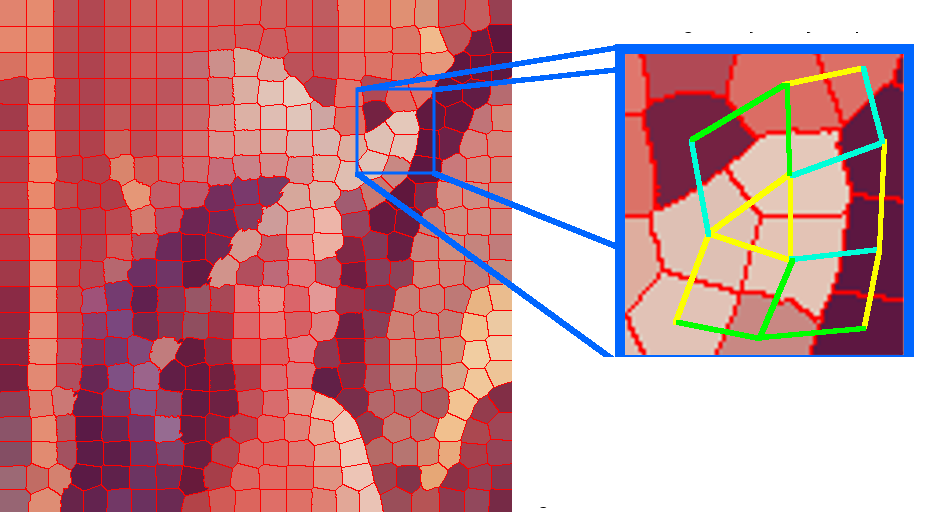
\includegraphics[scale=0.3]{figure/graphbased.png}
\captionof{figure}{Mô tả ảnh bằng đồ thị}
\end{center}
Các khái niệm quan trọng được sử dụng trong quá trình phân vùng sử dụng đồ thị là :
\begin{itemize}
\item Đỉnh kề: Hai đỉnh $v_i, v_j$ trong đồ thị được gọi là kề nhau nếu $(v_i,v_j)$ là cạnh của đồ thị. Bậc của một đỉnh $deg(v)$ là số cạnh nối với đỉnh $v$.
\item Đồ thị con và đồ thị riêng:
Đồ thị $G'=(V',E')$ là đồ thị con của đồ thị $G=(V,E)$ nếu $V' \subset V$ và $E'=E\cap (V',V')$ 
Đồ thị  $G''=(V,E')$ được gọi là đồ thị riêng của đồ thị $G=(V,E)$ nếu $E'\subset E$.
\item Cây bao chùm tối thiểu: Một cây được gọi là cây bao chùm tối thiểu của đồ thị $G$  nếu nó chứa tất cả các đỉnh của $G$ và trọng số nối mỗi đỉnh với một đỉnh bất kỳ là cạnh có trọng số nhỏ nhất trong các cạnh nối với đỉnh đó trong G. 
\item Vùng ảnh trên đồ thị: Với một phân vùng S, một vùng $C\in S$ tương ứng với một thành phần liên thông $G'=(V', E')$ trong đó  $V'\subset V, E' \subset E$ sao cho trong một vùng, trọng số nối hai cạnh bất kỳ nhỏ còn trọng số ứng với cạnh nối hai vùng có giá trị lớn.
\end{itemize}
\subsection{Các định nghĩa và tính chất liên quan}
Để có được việc phân vùng chúng ta cần xây dựng một tính chất để biết được có hay không môt ranh giới giữa hai vùng trong một phân vùng. Tính chất này được xây dựng thông qua việc so sánh sự khác nhau giữa các điểm ảnh trong cùng một vùng và sự khác nhau giữa các điểm ảnh giữa hai vùng dọc theo ranh giới giữa hai vùng.
Sự khác nhau trong nội tại vùng được định nghĩa là giá trị trọng số lớn nhất của cây bao trùm tối thiểu ứng với phần đồ thị tương ứng với vùng cần xét:
\begin{equation*}
Int(C)=\max_{e\in MST(C,E)}(w(e))
\end{equation*}
Sự khác nhau giữa các vùng được định nghĩa là trọng số nhỏ nhất của cạnh kết nối hai đỉnh đại diện cho hai vùng:
\begin{equation*}
Dif(C_1,C_2)=\min_{v_1\in C_1, v_2 \in C_2,(v_1, v_2) \in E}(w(v_i, v_j))
\end{equation*}

Trong trường hợp không có cạnh nối hai vùng thì $Dif(C_1,C_2)= \infty$. Gữa hai vùng sẽ có ranh giới nếu giá trị khác biệt giữa hai vùng lớn hơn giá trị khác biệt trong nội tại trong ít nhất 1 vùng. 
Chúng ta định nghĩa  sự khác biệt nội bộ tối thiểu của hai vùng $C_1, C_2$ được định nghĩa như sau: 
\begin{equation*}
Mint(C_1, C_2)= min(Int(C_1)+T(C_1),Int(C_2)+T(C_2))
\end{equation*}
với $T=\dfrac{k}{|C|}$, k là hằng số, $|C|$ là kích thước của vùng $C$. Lúc này ta có tính chất để xác định có tồn tại ranh giới phân vùng hay không giữa $C_1, C_2$  được định nghĩa như sau:
\begin{equation*}
D(C_1, C_2)=
\begin{cases}
 1, \textrm{Nếu } Dif(C_1, C_2)>Mint(C_1, C_2)\\
 0, \textrm{Trong trường hợp còn lại}\\
   \end{cases}
\end{equation*}
Trong thực tế $k$ không cố định và được chọn tùy vào ý kiến chuyên gia. Trong trường hợp $ k$ lớn thì kích thước các vùng đầu ra sẽ lớn, ngược lại kích thước đầu ra sẽ nhỏ. Giá trị của $k$ sẽ không nhỏ hơn kích thước  của vùng nhỏ nhất.
\chapter{Phương pháp phân vùng ảnh sử dụng biên động}
Mô hình biên động là một mô hình thành công nhất trong phân vùng ảnh. Các mô hình biên động hiện tại đang có có thể chia làm hai loại chính là: mô hình dựa trên cạnh (edge-based models), và mô hình dựa trên miền (region-based models). Cả hai loại này đều có ưu, nhược điểm riêng và việc lựa chọn cách nào còn tùy thuộc vào ứng dụng.

Ý tưởng của các phương pháp theo hướng tiếp cận này là xuất phát từ đường cong ban đầu, ta thực hiện biến đổi đường cong ban đầu theo thời gian  và dừng lại ở biên của vật. Việc biến đổi đường biên được thực hiện thông qua xây dựng một vòng lặp nhằm đạt được giá trị cuối cùng của đường cong thỏa mãn cực tiểu hoặc cực đại một hàm năng lượng (enery function) nào đó.

Mô hình dựa trên cạnh sử dụng gradient ảnh để dừng đường biên tại biên của vật. Mô hình dựa trên cạnh thường gồm hai thành phần dừng dựa trên cạnh  và thành phần lực cầu để kiểm soát chuyển động của đường biên. Thành phần dừng phục vụ cho việc dừng đường biên tại biên mong muốn. Thành phần lực cầu thực hiện co, mở rộng cạnh. Do vậy đường biên khởi tạo ban đầu có thể ở xa biên mong muốn. Khó khăn của mô hình này là việc lựa chọn lực cầu cho phù hợp. Nếu chọn lực cầu quá nhỏ, có thể quá trình phát triển biên sẽ không thể vượt qua một số vùng bằng phằng của đối tượng. Ngược lại nó có thể bỏ qua một số vùng biên yếu của vật.

Mô hình dựa trên miền có một số lợi thế so với mô hình dựa trên cạnh. Đầu tiên là việc mô hình dựa trên miền không sử dụng gradient ảnh do đó nó có hiệu suất tốt hơn đối với ảnh có biên yếu. Tiếp theo, nó ít ảnh hưởng bởi đường cong khởi tạo ban đầu hơn so với mô hình dựa trên cạnh.  Phần dưới đây sẽ là ba mô hình biên động dựa trên miền điển hình và một mô hình cải tiến kết hợp các lợi thế của các mô hình trên để giải quyết tốt hơn với các đầu vào đa dạng.
\section{Phương pháp Chan-Vese(CV)}


\subsection{Mô hình}
Chúng ta định nghĩa đường cong $C\in \Omega$ là biên của một tập con mở $\omega$ của $\Omega$. Giả sử rằng cường độ ảnh là tương đối đồng nhất và ảnh được chia làm hai vùng được xấp xỉ bởi các hằng số cường độ khác nhau $u_0^i$ và $u_0^0$. Đối tượng cần xác định trong ảnh được đại diện bởi vùng có cường độ $u_0^i$. Giả sử biên của nó là $C_0$. Vì vậy chúng ta có $u_0\approx u_0^i$ trong đối tượng, và $u_0\approx u_0^o$ ở ngoài đối tượng.
\begin{center}
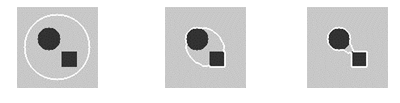
\includegraphics[scale=1]{figure/ytuong.png}
\captionof{figure}{Ý tưởng thuật toán}
\end{center}
Mô hình bao gồm 2 phần chính là thành phần khớp và thành phần chuẩn hóa: 

- Thành phần khớp: Đặt

\begin{center}
\begin{align*}
F_1=\iint_{inside(C)} |u_0-c_1|^2 \,dx\,dy\\
F_2=\iint_{inside(C)} |u_0-c_2|^2 \,dx\,dy
\end{align*}
\end{center}
Trong đó
\begin{center}
\begin{align*}
c_1=average(u_0 inside(C))\\
c_2=average(u_0 outside(C))
\end{align*}
\end{center} 
Hai thành phần $F_1, F_2$ được đưa ra nhằm so sánh sự khác nhau giữa cường độ ảnh trong cũng như ngoài đường cong đang xét so với cường độ ảnh với cường độ ảnh trong và ngoài đối tượng tương ứng. Trong trường hợp đường cong C bao phía ngoài đối tượng, ta có $F_1>0, F_2\approx 0$. Nếu đường cong $C$ nằm trong đối tượng ta có $F_1 \approx0, F_2> 0$. Nếu đường cong $C$ một phần nằm trong và một phần nằm ngoài đối tượng ta có $F_1>0, F_2> 0$. Nếu đường cong $C$ khớp với đối tượng $F_1 \approx 0, F_2\approx 0$:
\begin{center}
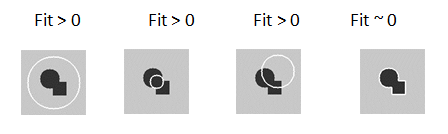
\includegraphics[scale=1]{figure/fitting.png}
\captionof{figure}{Thành phần khớp}
\end{center}
- Thành phần chuẩn hóa:
\begin{equation}
\mu .|C|+\nu .Area(inside(C))
\end{equation}
Trong đó $C$ là độ dài đường cong $C$, $Area(inside(C))$ là độ lớn phần diện tích giới hạn bởi đường cong. Trong hầu hết bài toán ta chọn $\nu=0$ và $\mu$ là tham số thay đổi tùy theo đầu vào để được kết quả tốt. Tham số $\mu $ được chọn càng nhỏ thì mô hình càng có khả năng phát hiện các đối tượng nhỏ. Trong trường hợp chỉ cần phát hiện các đối tượng có kích thước lớn, $\mu$ được chọn lớn hơn.\\

Tổng kết lại ta có hàm năng lượng: 

\begin{equation*}
\begin{split}
F(c_1, c_2, C)&=\mu .|C|+\nu .Area(inside(C)) \\ 
&+\lambda_1 .\iint_{inside(C)} |u_0-c_1|^2 \,dx\,dy\\
&+\lambda_2 .\iint_{outside(C)} |u_0-c_2|^2 \,dx\,dy
\end{split}
\end{equation*}
Bài toán cực tiểu đặt ra là
\begin{equation}
inf_{c_1,c_2,C} F(c_1, c_2, C)
\end{equation}
 
\subsection{Giải quyết bài toán sử dụng phương pháp tập mức}
Ta coi biên C được đại diện bởi tập mức 0 của một hàm $\phi: \omega \rightarrow \mathbb{R}$. Đặt 
\begin{equation*}
\begin{cases}
 C= \partial \omega ={(x,y)\in \Omega: \phi(x,y)=0}\\
 inside(C)= \omega={(x,y)\in \Omega: \phi(x,y)>0}\\
 outside(C)=\Omega \setminus \omega ={(x,y)\in \Omega: \phi(x,y)<0}
   \end{cases}
\end{equation*}
 \begin{center}
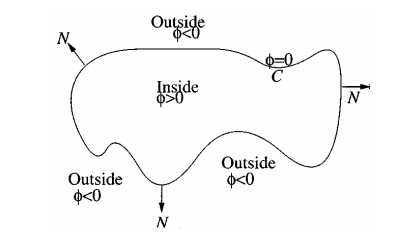
\includegraphics[scale=0.6]{figure/insideoutside.png}
\captionof{figure}{Đường cong $C=\{(x, y), \phi(x,y)=0 \}$}
\end{center}
Thay biến chưa biết C bởi biến chưa biết $\phi$.  Trong quá trình xây dựng lại phương trình theo $\phi$ ta sử dụng hàm Heviside $\phi$ và hàm Delta Dirac $\delta_0$
 \begin{equation*}
 H(z)=
\begin{cases}
 1 & \text{ nếu z>0}\\
0 & \text{ nếu z<0}
   \end{cases}
\end{equation*}
Hàm năng lượng sẽ được viết lại thành
\begin{equation*}
\begin{split}
F(c_1, c_2, C)&=\mu \int_{\Omega}\delta(x,y)|\nabla \phi(x,y)|\,dx\,dy+\nu  \int_{\Omega}H( \phi(x,y))\,dx\,dy \\ 
&+\lambda_1 .\int_{\Omega} |u_0-c_1|^2H(\phi(x,y)) \,dx\,dy\\&+\lambda_2 .\iint_{\Omega} |u_0-c_2|^2(1-H(\phi(x,y))) \,dx\,dy
\end{split}
\end{equation*}
Trong đó $c_1, c_2$ có thể được tính theo $\phi$ theo công thức:
\begin{equation*}
c_1(\phi)=\dfrac{\int_{\Omega}u_0(x,y)H(\phi(x,y))\,dx \,dy}{\int_{\Omega}H(\phi(x,y))\,dx\,dy}
\end{equation*}
\begin{equation*}
c_2(\phi)=\dfrac{\int_{\Omega}u_0(x,y)(1-H(\phi(x,y)))\,dx \,dy}{\int_{\Omega}H(\phi(x,y)1-H(\phi(x,y)))\,dx\,dy}
\end{equation*}
Để tính toán phương trình Euler-Lagrange cho hàm $\phi$ ta thực hiện mở rộng $H$ và $\delta_0$ tương ứng thành  $H_{\epsilon}$ và $\delta_{\epsilon}$, $\epsilon \rightarrow 0$. Hàm mở rộng $H_{\epsilon}$ có thể chọn là hàm $H_{1,{\epsilon}}$ trên $C^2(\bar{\Omega})$ của $H$ và $\delta_{\epsilon}=H'_{\epsilon}$:
\begin{equation*}
 H_{1,\epsilon}(z)=
\begin{cases}
 1 & \text{ nếu } z> \epsilon\\
0 & \text{ nếu } z <\epsilon \\
\dfrac{1}{2}(1+\dfrac{z}{\epsilon}+\dfrac{1}{\pi}\sin(\dfrac{\pi z}{\epsilon})) & \text{ nếu } z <|\epsilon|\\
   \end{cases}
\end{equation*}
Ngoài ra ta có thể sử dụng hàm mở rộng của H trên $C^{\infty}(\bar{\Omega})$:
\begin{equation*}
 H_{2,\epsilon}(z)=\dfrac{1}{2}(1+\dfrac{z}{\epsilon}+\dfrac{1}{\pi}\sin(\dfrac{\pi z}{\epsilon}))  \text{ nếu } z <|\epsilon|
\end{equation*}
Cả hai hàm $ H_{1,\epsilon}(z),  H_{2,\epsilon}(z)$ đều tiến dần đến $H$ và $ \delta_{1,\epsilon}(z),  \delta_{2,\epsilon}(z)$ đều tiến dần đến $\delta_0$ khi $\epsilon\rightarrow 0$. Tuy vậy điều khác nhau là $ \delta_{1,\epsilon}$ hỗ trợ ít hơn, cụ thể là trong đoạn $[-\epsilon, \epsilon]$ còn $ \delta_{2,\epsilon}$ lại khác 0 tại mọi điểm. Do hàm năng lượng không lồi do vậy có thể có cực trị địa phương, và kết quả có thể phụ thuộc vào đường cong khởi tạo ban đầu. Với $H_{1,\epsilon}(z), \delta_{1,\epsilon}(z)$ thuật toán có thể đưa ra kết quả là cực trị địa phương, trong khi với $H_{2,\epsilon}(z), \delta_{2,\epsilon}(z)$ thuật toán có xu hướng đưa ra kết quả là cực trị toàn cục.

 Hàm mở rộng của $F(c_1,c_2,C)$ thành
\begin{equation*}
\begin{split}
F(c_1, c_2, \phi)&=\mu \int_{\Omega}\delta_{2,\epsilon}(x,y)|\nabla \phi(x,y)|\,dx\,dy+\nu  \int_{\Omega}H_{2,\epsilon}( \phi(x,y))\,dx\,dy \\ 
&+\lambda_1 .\int_{\Omega} |u_0-c_1|^2H_{2,\epsilon}(\phi(x,y)) \,dx\,dy\\&+\lambda_2 .\iint_{\Omega} |u_0-c_2|^2(1-H_{2,\epsilon}(\phi(x,y))) \,dx\,dy
\end{split}
\end{equation*}
Cố định $c_1, c_2$, thực hiện cực tiểu hàm $F_{\epsilon}$ theo $\phi$, ta thu được phương trình Euler-Lagrange theo $\phi$. Tham số hóa $\phi$ theo thời gian và áp dụng phương pháp hướng giảm ta được:
\begin{equation}
\dfrac{\partial \phi}{\partial t}= \delta_{2,\epsilon}(\phi)[\mu- div(\dfrac{\nabla \phi}{|\nabla \phi|})- \nu- \lambda_1 (u_0-c_1)^2-\lambda_2 (u_0-c_2)^2]  \text{ trong } (0,\infty)\times \Omega
\end{equation}
\begin{equation}
\phi(0,x,y)=\phi_0(x,y) \text{ trong } \Omega 
\end{equation}
\begin{equation}
\dfrac{\delta_{\epsilon}(\phi)}{|\nabla \phi|}\dfrac{\partial \phi}{\partial \vec{n}}=0
\end{equation}

Trong đó $\vec{n}$ là vector pháp tuyến hướng ra ngoài của biên $\Omega$, và $\dfrac{\partial \phi}{\partial \vec{n}} $ là đạo hàm theo vector pháp tuyến của $\phi$. Trong quá trình tính toán xấp xỉ các giá trị $\phi_x, \phi_y$ ở các điểm gần biên, ta cần biết được giá trị $\phi(x,y)$ tại các điểm $(x, y)$ nằm ngoài biên $\partial \Omega$ trong khi ta chỉ có giá trị tại các điểm nằm trong và trên biên của $\Omega$, một cách tự nhiên người ta có thể chọn $\phi(x,y)$ tại các điểm $(x, y)$ nằm ngoài biên bằng với giá trị của $\phi(x,y)$ tại điểm gần $(x,y)$  nhất trên biên, hay $\dfrac{\partial \phi}{\partial \vec{n}}=0$. Khi làm việc với hàm Level set, thủ tục cần thiết là khởi tạo lại hàm $\phi$ bằng hàm dấu khoảng cách ứng với $\phi$. Trong quá trình cập nhật $\phi$, nó sẽ được điều chỉnh để khớp với biên của vật. Tuy nhiên trong quá trình cập nhật dải giá trị của $\phi$: ($max(\phi)-min(\phi)$) sẽ thay đổi. Điều này sẽ dẫn đến vấn đề  khi số bước lặp lớn dải giá trị của $\phi$ sẽ tăng dần  dẫn đến có thể không thể tiếp tục tính toán do hạn chế về số chữ số chính xác có thể tính toán được. Do đó quá trình tiến hóa $\phi$ có thể trở nên thiếu chính xác hoăc $\phi$ dừng hẳn quá trình tiến hóa. Vấn đề này có thể giải quyết bằng việc khởi tạo lại hàm phi bằng hàm dấu khoảng cách (signed distance function) . Hàm $\phi$ sẽ được khởi tạo thành hàm khác với các giá trị tương ứng bằng khoảng cách tới điểm gần nhất trên đường mức 0 ứng với $\phi$, đồng thời có dấu giống với dấu tương ứng với giá trị của $\phi$. Việc tính toán hàm dấu khoảng cách này có thể được thực hiện qua một số bước lặp với việc giải hệ phương trình sau:
\begin{equation}
\begin{cases}
 \psi^{\tau}=sign(\phi^n)(1-|\nabla \phi|)\\
 \psi^{0}=\phi^n
   \end{cases}
\end{equation}
 Trong đó $\phi^{\tau}$ là hàm dấu khoảng cách thu được ở bước $\tau$, $\psi^{0}$ là hàm dấu khoảng cách khởi tạo ban đầu. Cuối cùng ta có thuật toán như sau:
\begin{itemize}
\item Bước 1: Khởi tạo $\phi^0=\phi_0, n=0$
\item Bước 2: Tính toán các giá trị $c_1(\phi^n), c_2(\phi^n)$
\item Bước 3: Giải phương trình đạo hàm riêng (3.3) để có $\phi^{n+1}$
\item Bước 4: Khởi tạo lại hàm $\phi$ bằng hàm dấu khoảng cách tới đường cong
\item Bước 5: Kiểm tra điều kiện dừng, nếu không thỏa mãn thì gán $n=n+1$ và quay lại bước 2
\end{itemize}
Các tính toán xấp xỉ được dùng trong quá trình giải số hệ phương trình đạo hàm riêng (3.16) như sau:
\begin{equation}
\begin{split}
&k=div(\dfrac{\nabla \phi}{|\phi|})=\dfrac{\phi_{xx}\phi^2_{y}-2\phi_{xy}\phi_{x}\phi{y}+\phi_{yy}\phi^2_{x}}{(\phi^2_x+\phi^2_y)^{3/2}}\\
&\phi_x\approx \dfrac{1}{2h}(\phi_{i+1,j}-\phi_{i-1,j}) \\ 
&\phi_x\approx \dfrac{1}{2h}(\phi_{i,j+1}-\phi_{i,j-1}) \\
&\phi_{xx}\approx \dfrac{1}{h^2}(\phi_{i+1,j}-\phi_{i,j}+\phi_{i-1,j}) \\
&\phi_{yy}\approx \dfrac{1}{h^2}(\phi_{i,j+1}-\phi_{i,j}+\phi_{i,j-1}) \\
&\phi_{xy}\approx \dfrac{1}{h^2}(\phi_{i+1,j+1}-\phi_{i-1,j+1}-\phi_{i,j+1}+\phi_{i,j-1}) 
\end{split}
\end{equation}
trong đó $h$ là khoảng cách lưới. Khi đó (7) có thể được rời rạc hóa thành thành: 
\begin{equation}
\dfrac{\phi_{n+1}-\phi_{n}}{\Delta t}=\delta_{\epsilon}(\phi_{n})[\mu -\lambda_1 (u_{i,j}-c_1(\phi^{n}))^2+\lambda_2 (u_{i,j}-c_2(\phi^{n}))^2]
\end{equation}
Từ đó ta có thể tính được $\phi^{n+1}$ theo $\phi_{n}$
Chú ý là thành phần $|C|$ có thể viết lại dưới dạng tổng quát hơn thành $|C|^p$. Nếu ta xét đến trường hợp số chiều $N>1(\Omega \in \mathbb{R}^N )$, khi đó ta có thể chọn $p=1$ hoặc $p=\dfrac{N}{N-1}$
\subsection{Ưu nhược điểm của mô hình}
\hspace{0.5cm}Ưu điểm của mô hình là có thể phát hiện được biên trơn, xử lý tốt với ảnh nhiễu, mô hình có thể phát hiện được biên từ duy nhất một đường cong khởi tạo ban đầu. Đường cong này có thể ở mọi vị trí trên ảnh mà không nhất thiết phải bao quanh đối tượng trong ảnh.

Nhược điểm của mô hình  là độ phức tạp tính toán còn lớn do thao tác re-initialization và kết quả còn thiếu chính xác trong trường hợp ảnh không đồng nhất cường độ. Điều này có thể giải thích là do việc coi giá trị mức xám của các điểm trong đối tượng, ngoài đối tượng là đồng nhất, trong khi sự chênh lệch giữa mức xám giữa các điểm ảnh lại lớn trong trường hợp ảnh không đồng nhất cường độ.

%\begin{wrapfigure}{r}{0.5\textwidth}
%  \caption{Kết quả với ảnh không đồng nhất cường độ}
%  \centering
%    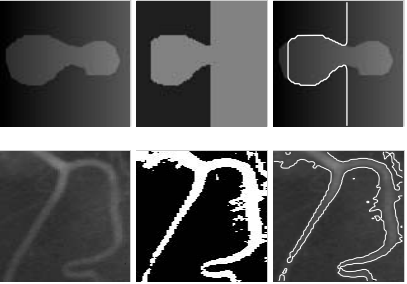
\includegraphics[width=0.5\textwidth]{figure/mistake.png}
%\end{wrapfigure}
\begin{center}
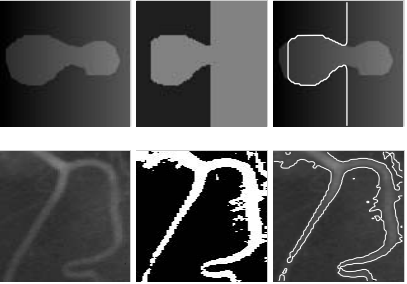
\includegraphics[]{figure/mistake.png}
\captionof{figure}{Kết quả của mô hình C-V trong trường hợp ảnh không đồng nhất}
\end{center}

\section{Phương pháp Local binary fiting energy (LBF)}
Phần trên đã đề cập đến việc mô hình CV tỏ ra không hiệu quả đối với ảnh không đồng nhất cường độ do mô hình CV chỉ sử dụng thông tin toàn cục của ảnh. Mô hình LBF được tạo ra để giải quyết vấn đề này. Mô hình LBF sử dụng thêm thông tin địa phương nhờ việc sử dụng cửa sổ Gauss thông qua sử dụng hàm nhân Gauss.
\subsection{Mô hình}
\hspace{0.5cm}Cho ảnh $I: \Omega \rightarrow \mathbb{R}^d$. Trong đó $\Omega \subset \mathbb{R}^2$  là miền ảnh, $d>1$ là bậc của vector $I(x)$. Với ảnh xám d=1, với ảnh màu d=3. Gọi $C$ là biên của ảnh trong $\Omega$, với mỗi x ta đinh nghĩa một hàm năng lượng sau:
\begin{equation}
\begin{split}
\epsilon_x^{LBF}(C, f_1(x), f_2(x))=&\lambda_1 \int_{in(C)} K(x-y)|I(y)-f_1(x)|^2\,dy\\
									&+ \lambda_2 \int_{out(C)} K(x-y)|I(y)-f_2(x)|^2\,dy 
\end{split}
\end{equation}
trong đó $\lambda_1, \lambda_2$ là các hằng số dương, $K$ là hàm nhân với thuộc tính địa phương $K(u)$ giảm và dần về 0 khi |u| giảm, $f_1(x), f_2(x)$ là hai số khớp với cường độ ảnh taị các điểm gần x. Ta gọi x là điểm trung tâm của hàm năng lượng trên. Trong mô hình này $K$ được chọn là hàm nhân Gaussian
\begin{equation*}
K_{\sigma}(x)=\dfrac{1}{(2\pi)^{n/2}\sigma^n}e^{-|x|^2/2\sigma^2}
\end{equation*}
với $\sigma$ là tham số dương có thể tùy chỉnh được. Nhấn mạnh rằng $f_1(x), f_2(x)$ thay đổi theo x. $f_1(x), f_2(x)$ làm phương pháp này trở nên khác các phương pháp khác.
\begin{center}
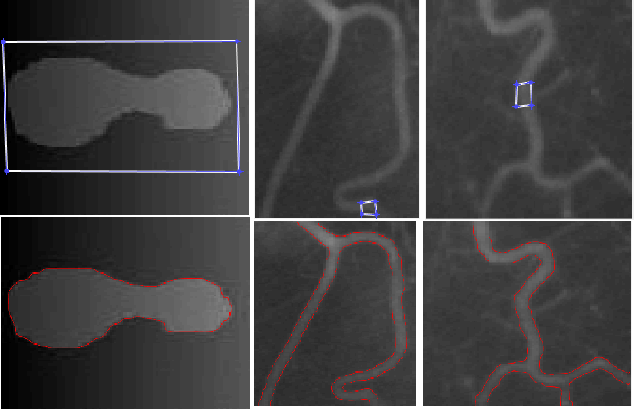
\includegraphics[scale=0.7]{figure/LBFresult.png}
\captionof{figure}{Kết quả của mô hình LBF trong trường hợp ảnh không đồng nhất}
\end{center}

Trong mô hình này, hàm năng lượng có tính đại phương với $x$ hay $f_1(x)$, $f_2(x)$  chỉ khớp với cường độ ảnh tại các điểm gần $x$. Điều này có được là do tính chất của hàm $K$ là $K(x-y)$ có giá trị lớn hơn khi y gần $x$. Vì vậy cường độ ảnh tại các điểm $y$ gần $x$ ảnh hưởng nhiều hơn đến giá trị $f_1, f_2$ làm cực tiểu hàm năng lượng $\epsilon_x^{LBF}(C,f_1, f_2)$, trong khi cường độ ảnh tại các điểm y xa x hầu như không ảnh hưởng tới các giá trị $f_1, f_2$.
%%Ảnh nhiễu


\begin{figure}[]
\def\tabularxcolumn#1{m{#1}}
%
\begin{tabular}{cc}
\subfloat[Đường cong khởi tạo]{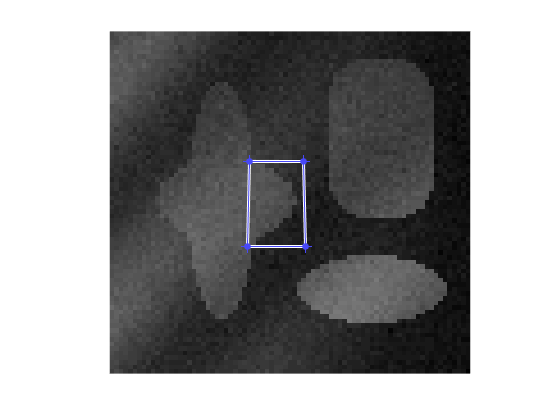
\includegraphics[width=7cm]{figure/noisyinit.png}} 
   & \subfloat[Bước lặp 10]{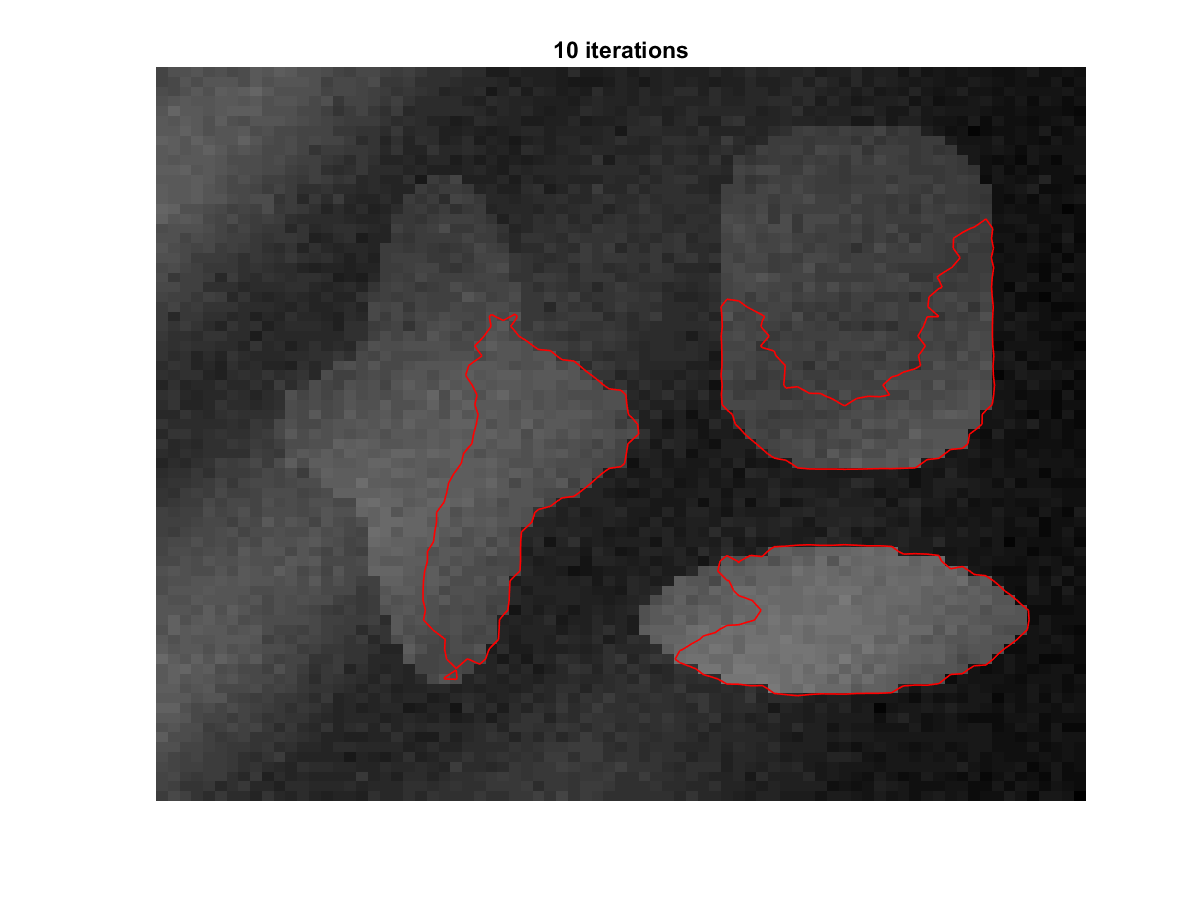
\includegraphics[width=7cm]{figure/noisy10.png}}\\  
    \subfloat[Bước lặp 30]{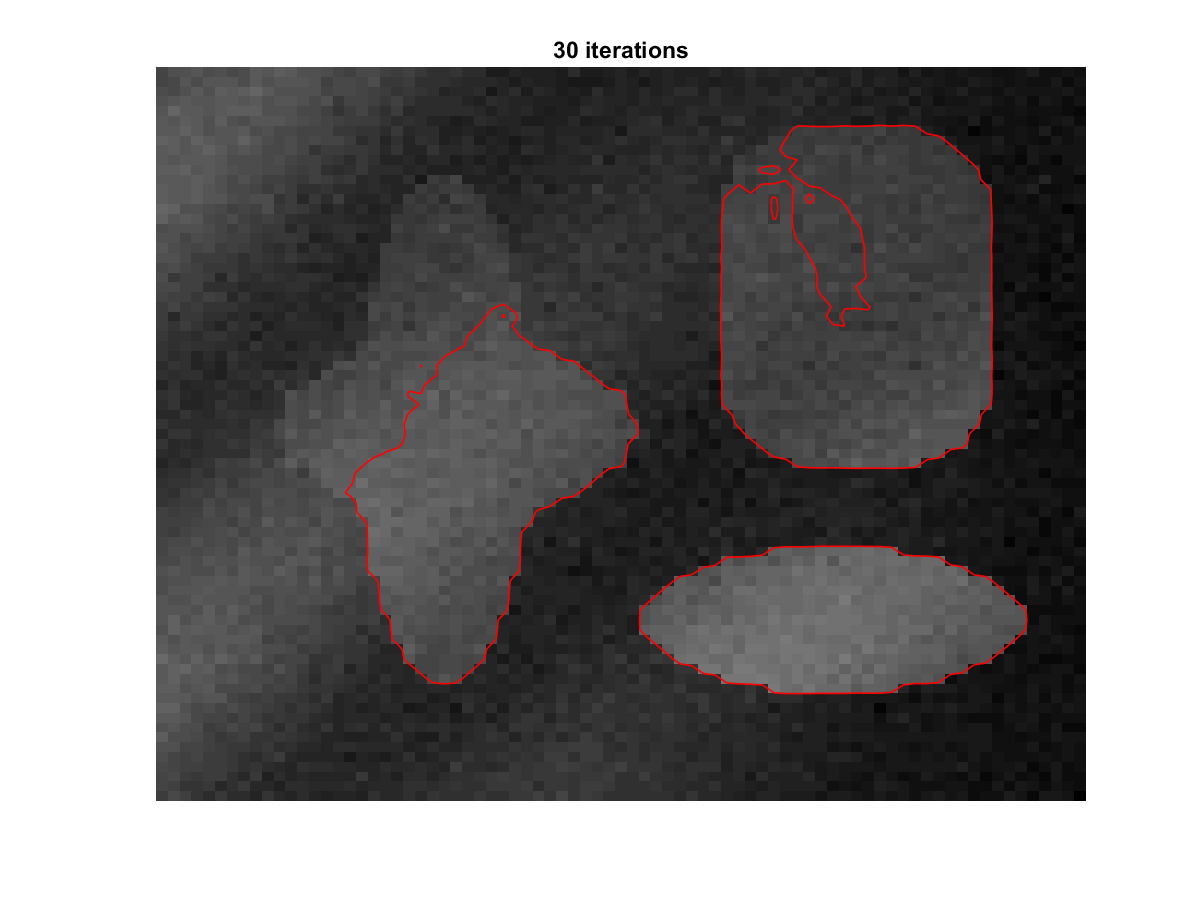
\includegraphics[width=7cm]{figure/noisy30.png}} 
   & \subfloat[Bước lặp 130]{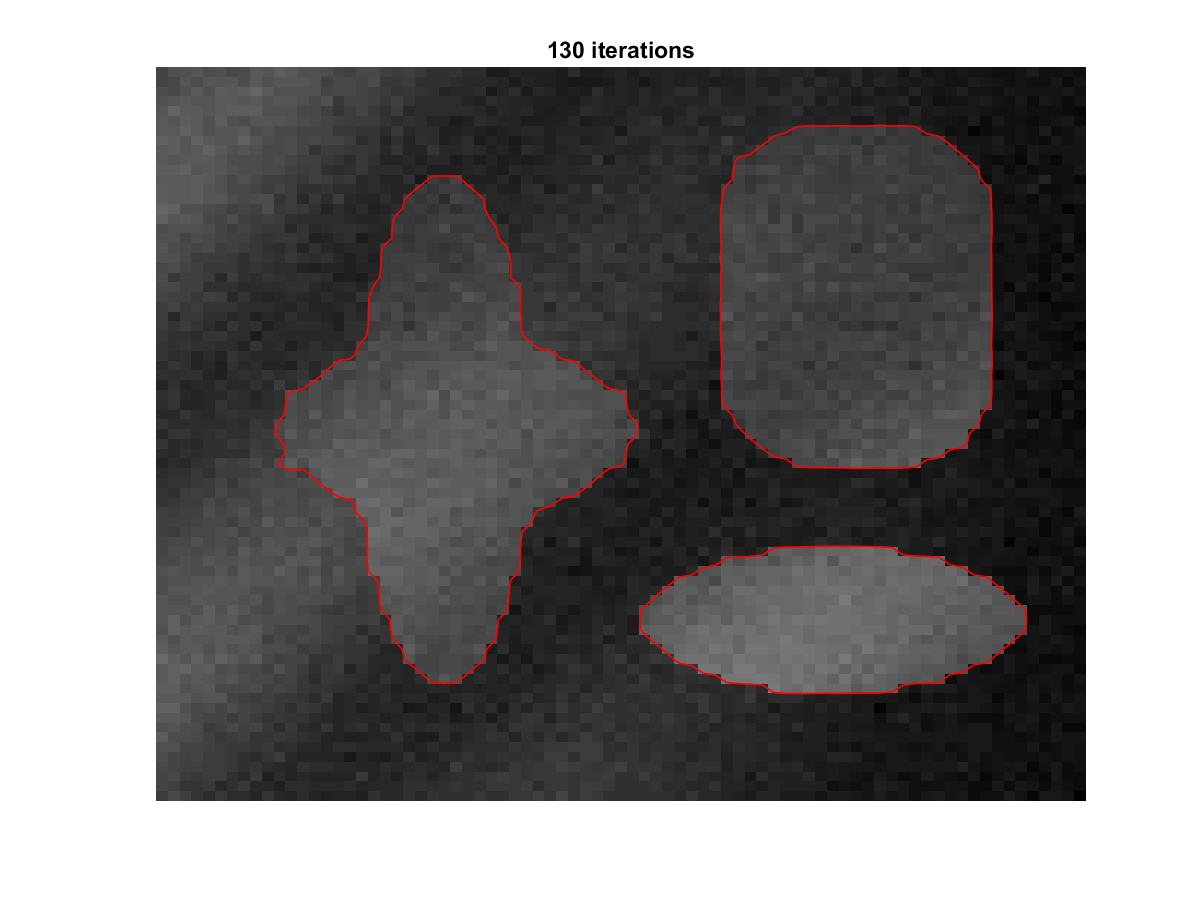
\includegraphics[width=7cm]{figure/noisy130.png}}    
   \end{tabular}


\caption{Kết quả LBF  với ảnh nhiễu}\label{foo}
\end{figure}
Tại mỗi điểm trung tâm x, hàm năng lượng $\epsilon_x^{LBF}(C,f_1, f_2)$   có thể đạt cực tiểu khi đường con C khớp với biên của đối tượng và các giá trị $f_1, f_2$ được chọn sao tối ưu. Tuy nhiên hàm năng lượng $\epsilon_x^{LBF}(C,f_1, f_2)$ được định nghĩa một cách cục bộ theo điểm trung tâm x. Để tìm được toàn bộ biên của vật, ta cần cực tiểu hàm $\epsilon_x^{LBF}$  với mọi x trong miền ảnh $\Omega$. Điều này có thể làm được bằng cách định nghĩa hàm năng lượng mới sau:
\begin{equation}
\epsilon(C, f_1, f_2)=\int_{\Omega} \epsilon_x^{LBF}(C, f_1(x), f_2(x))\,dx
\end{equation}
\subsection{Giải quyết bài toán sử dụng phương pháp tập mức}
Đường cong $C \subset \Omega$ được đại diện bởi tập mức 0 của một hàm Lipschit $\phi \rightarrow \mathbb{R}$. Viết lại hàm năng lượng $\epsilon_x^{LBF}(C,f_1, f_2)$ theo $\phi$ ta được:
\begin{equation*}
\begin{split}
\epsilon_x^{LBF}(\phi, f_1(x), f_2(x))
=&\lambda_1 \int_{\Omega} K_{\sigma}(x-y)|I(y)-f_1(x)|^2H(\phi(y))\,dy\\ &+ \lambda_2 \int_{\Omega} K_{\sigma}(x-y)|I(y)-f_2(x)|^2(1-H(\phi(y)))\,dy 
\end{split}
\end{equation*}
trong đó $H$ là hàm Heaviside. Theo đó hàm năng lượng $\epsilon^{LBF}$ có thể được viết lại thành
\begin{equation*}
\begin{split}
\epsilon(C, f_1, f_2)&=\int_{\Omega} \epsilon_x^{LBF}(C, f_1(x), f_2(x))\,dx\\
&=\lambda_1 \int[\int K_{\sigma}(x-y)|I(y)-f_1(x)|^2H(\phi(y))\,dy]\,dx \\
&+ \lambda_2 \int[\int K_{\sigma}(x-y)|I(y)-f_2(x)|^2(1-H(\phi(y)))\,dy ]\,dx
\end{split}
\end{equation*}
Để đảm bảo rằng $\phi$ ổn định, chúng ta thêm hàm độ lệch giữa hàm tập mức $\phi$ và hàm dấu khoảng cách.
\begin{equation*}
P(\phi)= \int_{\Omega}\dfrac{1}{2}(|\nabla \phi|-1)^2\,dx
\end{equation*}
\begin{equation*}
\mathcal{L}(\phi)=\int_{\Omega}\delta(\phi(x))|\nabla \phi(x)|\,dx
\end{equation*}
Bây giờ ta có hàm energy cuối cùng
\begin{equation*}
\mathcal{F}(\phi,f_1,f_2)=\epsilon(C, f_1, f_2)+\mu \mathcal{P}(\phi)+\nu \mathcal{L}(\phi)
\end{equation*}
trong đó $\mu$ và $\nu$ là các hằng số. Trong thực tế, các $H$ được xấp xỉ bởi một hàm trơn $H_{\epsilon}$
\begin{equation*}
H_{\epsilon}(x)=\dfrac{1}{2}[1+\dfrac{2}{\pi}\arctan(\dfrac{x}{\epsilon})]
\end{equation*}
và $\delta_{\epsilon}(x)$ được chọn là
\begin{equation*}
\delta_{\epsilon}(x)=H_{\epsilon}'(x)=\dfrac{1}{\pi}\dfrac{\epsilon}{\epsilon^2+x^2}
\end{equation*}
Hàm năng lượng này sẽ được cực tiểu hóa để tìm biên 
Với $\phi$ cố định ta thực hiện cực tiểu hàm năng lượng $\epsilon(C, f_1, f_2)$  theo $f_1, f_2$ ta tìm được $f_1, f_2$ như sau:
\begin{equation}
f_1(x)=\dfrac{K_{\sigma}*[(H_{\epsilon}(\phi(x)))*I(x)]}{K_{\sigma}*(H_{\epsilon}(\phi(x))}
\end{equation}
\begin{equation}
f_1(x)=\dfrac{K_{\sigma}*[(1-H_{\epsilon}(\phi(x)))*I(x)]}{K_{\sigma}*(1-H_{\epsilon}(\phi(x))}
\end{equation}
Theo công thức $f_1, f_2$ ở trên luôn dương do $H_{\epsilon}$ và $1-H_{\epsilon}$ luôn dương. Cố định $f_1, f_2$ và cực tiểu hàm $\epsilon^{LBF}(\phi, f_1(x), f_2(x))$ theo $\phi$, sử dụng phương pháp hướng giảm ta được:

\begin{equation*}
\begin{split}
\dfrac{\partial \phi}{\partial t}=&- \delta_{\epsilon}(\phi)(\lambda_1 e_1 -\lambda_2 e_2)+\nu \delta_{\epsilon}(\phi)div(\dfrac{\nabla \phi}{|\nabla \phi|})\\
&+\mu(\nabla^2 \phi -div(\dfrac{\nabla \phi}{|\nabla \phi|}))
\end{split}
\end{equation*} 
trong đó $\delta_{\epsilon}(x)$ là hàm trơn Dirac được cho như công thức trên và $e_1(x), e_2(x)$ được tính theo công thức sau:
\begin{equation*}
e_1(x)=\int_{\Omega}K_{\sigma}(y-x)|I(x)-f_1(y)|^2 \,dy
\end{equation*}
\begin{equation*}
e_1(x)=\int_{\Omega}K_{\sigma}(y-x)|I(x)-f_2(y)|^2 \,dy
\end{equation*}
Ta sẽ có thuật toán như sau:
\begin{itemize}
\item Bước 1: Khởi tạo $\phi^0=\phi_0, n=0$
\item Bước 2: Tính toán các giá trị $c_1(\phi^n), c_2(\phi^n)$
\item Bước 3: Giải phương trình đạo hàm riêng (1.14) để có $\phi^{n+1}$
\item Bước 4: Kiểm tra điều kiện dừng, nếu không thỏa mãn thì gán $n=n+1$ và quay lại bước 2
\end{itemize}
\subsection{Ưu nhược điểm của mô hình}
Ưu điểm của mô hình này là không cần thiết phải chuẩn hóa $f_1, f_2$. Thực tế, $f_1, f_2$ làm cực tiểu hàm năng lượng có thể được cho bởi công thức (3.11)(3.12) và là các hàm trơn. Hơn nữa mô hình này cũng không cần phải mở rộng $f_1, f_2$ vì nó được định nghĩa trên toàn miền ảnh $\Omega$. Một ưu điểm nữa của mô hình này là việc khởi tạo lại hàm $\phi$ là không cần thiết do việc thêm hàm chuẩn hóa khoảng cách. Nhờ việc chuẩn hóa khoảng cách này mà việc khởi tạo hàm $\phi$ lúc đầu trở nên linh hoạt hơn. Một trường hợp đặc biêt là ta hoàn toàn có thể khởi tạo hàm $\phi$ là hàm nhị phân, nhận giá trị $c_0$ ngoài miền $R_0$, nhận giá trị $-c_0$ ở trong miền $R_0$.

Ngoài việc phục vụ cho việc phân vùng, mô hình LBF còn có thể sử dụng cho việc khử nhiễu. Hình (3.7) là kết quả của mô hình LBF với ảnh màu, giải thích cho sự kết hợp giữa phân vùng và khử nhiễu được sử dụng trong mô hình LBF. Dòng đầu tiên là kết quả của LBF từ đường cong khởi tạo cho đến kết quả cuối cùng sau khi phân vùng. Dòng 2 và dòng 3 là kết quả tương ứng với ảnh $f_1, f_2$ được tính theo công thức $(3.11)(3.12)$. Chúng ta định nghĩa một ảnh khớp sau dựa trên $f_1, f_2, \phi$:
\begin{equation*}
f=H_{\epsilon}(\phi)f_1+(1-H_{\epsilon}(\phi))f_2
\end{equation*}
$f$ có thể dùng sử dụng để xấp xỉ ảnh gốc trong quá trình khử nhiễu. Dòng thứ 4 trong hình $(3.5)$ là kết quả của quá trình tiến hóa $f$. Khi hàm $\phi$ hội tụ ta có $f$ khớp với ảnh gốc và đồng thời khử được nhiễu của ảnh gốc ban đầu. 

\begin{center}
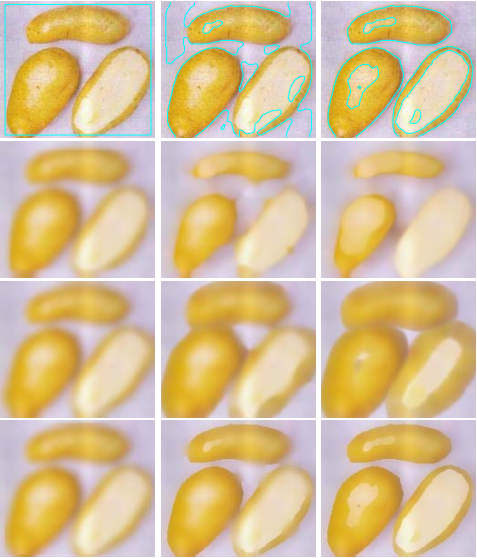
\includegraphics[]{figure/denoise.png}
\captionof{figure}{Khử nhiễu với mô hình LBF}
\end{center}

Một nhược điểm của mô hình là quá trình  tính toán $\lambda_1 e_1 -\lambda_2 e_2$ còn tốn nhiều tài nguyên. Điều này có thể khắc phục nhờ việc dùng mô hình LIF sẽ được trình bày tiếp theo.
\section{Phương pháp Local image fitting(LIF)}
Ở phần trước chúng ta đã thấy được mô hình LBF phân vùng hiệu quả với ảnh không đồng nhất cường độ, đồng thời hiệu suất của mô hình LBF cũng tốt hơn trong cả độ chính xác của kết quả cũng như tốc độ tính toán. Phần dưới đây sẽ trình bày về mô hình LIF với khả năng xử lý với ảnh không đồng nhất cường độ xám, sử dụng thông tin địa phương của ảnh để xây dựng hàm năng lượng dựa trên sự khác nhau của ảnh đã khớp so với ảnh ban đầu. Mô hình LIF thực hiện chuẩn hóa hàm tập mức bằng việc sử dụng hàm lọc Gauss sau mỗi vòng lặp. Điều này cũng giúp cho phương pháp này tránh khỏi quá trình khởi tạo lại hàm tập mức bằng dấu khoảng cách. Kết quả thực nghiệm đã cho thấy tốc độ khi thực hiện phân vùng với mô hình này tốt hơn so với mô hình LBF trong khi đưa ra một kết quả phân vùng tương đương.
\subsection{Mô hình và phương trình với tập mức}
Một hàm khớp địa phương được định nghĩa như sau:
\begin{equation*}
I^{LFI}= m_1H_{\epsilon}(\phi)+m_2(1-H_{\epsilon}(\phi))
\end{equation*}
Trong đó $m_1,m_2$ được định nghĩa như sau
\begin{equation*}
\begin{cases}
 m_1=mean(I\in (\{x\in \Omega|\phi(x)<0\}\cap W_k(x)))\\
  m_2=mean(I\in (\{x\in \Omega|\phi(x)>0\}\cap W_k(x)))
   \end{cases}
\end{equation*}
\begin{center}
\includegraphics[scale=.7]{figure/3clif1.png}
\captionof{figure}{Phân vùng với ảnh nhiều đối tượng có mức xám khác nhau}
\end{center}
trong đó $W_k(x)$ là một hàm cửa sổ hình chữ nhật. Ở đây ta chọn $W_k(x)$  là hàm cửa sổ Guassian $K_{\sigma}(x)$ với độ lệch chuẩn $\sigma$ và với kích thước $4k+1$ và $4k+1$ với $k$ là số nguyên lớn nhất không vượt quá $\sigma$. Việc sử dụng cửa sổ này thể hiện tính chất địa phương của mô hình. Việc tính $m_1, m_2$ chỉ thực hiện với vùng nằm trong cửa sổ mà không phải thực hiện trên toàn vùng như mô hình CV. Nhờ tính chất này mà mô hình LIF có thể xử lý được với ảnh không đồng nhất cường độ, ngoài ra còn có thể phân vùng với ảnh nhiều đối tượng với các cường độ xám khác nhau. Mô hình này sử dụng hàm năng lượng khớp địa phương thể hiện độ lệch giữa ảnh sau khi khớp và ảnh gốc:
\begin{equation*}
E^{LIF}(\phi)=\dfrac{1}{2}\int_{\Omega}|I(x)-I^{LFI}(x)|^2\,dx
\end{equation*}
\begin{center}
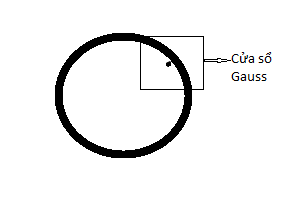
\includegraphics[]{figure/Gaussfilter.png}
\captionof{figure}{Cửa sổ Gauss}
\end{center}
Thêm thành phần biến thiên $\eta$ vào hàm $\phi$ ta được $\bar{\phi}=\phi+\epsilon \eta$
Cố định $c_1, c_2$ . Đạo hàm theo $\phi$ và cho $\epsilon$ tiến dần tới 0 ta có
\begin{equation*}
\begin{split}
\dfrac{\delta E^{LIF}}{\delta \phi } &=\lim_{\epsilon \rightarrow 0}\dfrac{d}{d \epsilon}(\dfrac{1}{2}\int_{\Omega}|I(x)-m_1H_{\epsilon}(\bar{\phi})-m2(1-H_{\epsilon}(\bar{\phi}))|^2\,dx) \\ 
&=\lim_{\epsilon \rightarrow 0}\dfrac{d}{d \epsilon}(-\int_{\Omega}-\delta_{\epsilon}(\phi)(I(x)-m_1H_{\epsilon}(\bar{\phi})-m2(1-H_{\epsilon}(\bar{\phi})))(m_1-m_2)\eta\,dx) \\ 
&=-(\int_{\Omega}-\delta_{\epsilon}(\phi)(I(x)-m_1 H_{\epsilon}(\phi)-m2(1-H_{\epsilon}(\phi)))(m_1-m_2)\eta\,dx)
\end{split}
\end{equation*}
Theo đó ta có phương trình Euler-Lagarange:
\begin{equation*}
\delta_{\epsilon}(\phi)\{(I-I^{LFI})(m_1-m_2)\}=0
\end{equation*}
Sử dụng phương pháp hướng giảm ta có
\begin{equation*}
\dfrac{\partial \phi}{\partial t}=(I-I^{LFI})(m_1-m_2)\delta_{\epsilon}(\phi)
\end{equation*}
Trong quá trình làm việc theo phương pháp với tập mức, để đảm bảo tính hội tụ của $\phi$, ta cần thực hiện thao tác khởi tạo lại $\phi$. Tuy nhiên việc này đòi hỏi khá nhiều tài nguyên. Mô hình này thực hiện việc khởi tạo lại thành chuẩn hóa hàm $\phi$ sử dụng hàm chuẩn hóa Gauss $\phi=\phi* G_{\psi}$, trong đó $\psi$ là độ lệch chuẩn.

Các bước của thuật toán như sau:
\begin{itemize}
\item Bước 1: Khởi tạo hàm $\phi$ là hàm nhị phân như sau:
\begin{equation*}
\phi_(x,t=0)=\begin{cases}
-\rho, x\in \Omega_0 -\partial \Omega_0\\
0, x\in \partial \Omega_0\\
\rho, x\in \Omega- \Omega_0
\end{cases}
\end{equation*}
 trong đó $\rho>0$ là hằng số, $\Omega_0$ là tập con  của miền ảnh $\Omega$ và $\partial \Omega_0$ là biên của $\Omega_0$
 \item Bước 2: Tính toán $\phi$ sử dụng phương trình (3.43)
 \item Bước 3: Chuẩn hóa hàm tập mức $\phi$ bởi hàm nhân Gaussian. Ví dụ $\phi=\G_{\psi}*\phi$ trong đó $\psi$ là độ lệch chuẩn thỏa mãn lớn hơn $\sqrt{t}$ để tăng cường khả năng làm mịn
 \item Bước 4: Kiểm tra điều kiện dừng, nếu không thỏa mãn quay lại bước 2
\end{itemize}
Qua quá trình thử nghiệm, tham số $\psi$ ở bước 3 thường được chọn trong khoảng 0.45 đến 1, nếu nhiễu lớn thì $\psi$ nên chọn lớn hơn.
Ngoài việc sử dụng hàm lọc Gauss cho để loại bỏ thao tác khởi tạo lại hàm $\phi$, chúng ta hoàn toàn có thể sử dụng kỹ thuật thêm thành phần hàm phạt như mô hình LBF. Tuy nhiên thực tế cho thấy kết quả khi làm theo cách sử dụng hàm phạt này nhiều khi cho ra biên không mong muôn. Điều này có thể được giải thích là do việc thêm hàm phạt chỉ thỏa mãn điều kiện cần chứ không phải điều kiện đủ, dẫn đến khi sử dụng hàm phạt kết hợp với hàm năng lượng ban đầu làm cho mô hình dễ dẫn tới cực trị địa phương.
\subsection{Ưu nhược điểm của mô hình}
So với mô hình LBF, tuy mô hình LBF không cần thao tác re-initialization không cần thiết, tuy nhiên độ phức tạp tính toán còn tương đối cao. Chi phí tính toán của mô hình LBF chủ yếu nằm ở thao tác tính toán $\lambda_1 e_1-\lambda_2 e_2$. Mô hình LIF có tốc độ tính toán tốt hơn hiều so với LBF. Đồng thời thực nghiệm cho thấy mô hình LIF có thể đạt tới việc phân chia nhỏ hơn pixel(Hình 3.10). Hình 3.10 cho thấy với phương pháp C-V kết quả cuối cùng thu được 2 ngón tay ở giữa bị dính vào nhau trong khi với phương pháp LIF thì chúng tách rời hoàn toàn.
\begin{center}
\begin{figure}
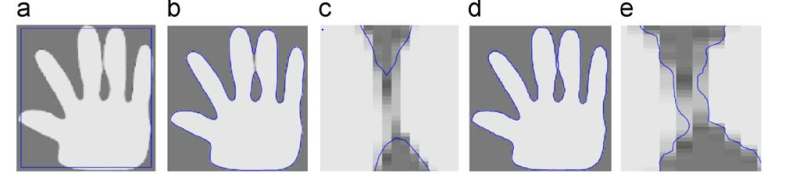
\includegraphics[scale=0.7]{figure/subpixel.png}
\caption{Hình b và c thể hiện kết quả của phương pháp C-V, hình  d và e thể hiện kết quả của phương pháp LIF}
\end{figure}

\end{center}   
\section{Mô hình kết hợp Global và Local}
\subsection{Mô hình}
Cả 3 phương pháp phân vùng sử dụng biên động như đã trình bày ở trên đều có ưu nhược điểm của riêng mình. Với mô hình CV, nó hoạt động tốt với các ảnh mà cường độ xám trong và ngoài đối tượng trong ảnh đồng nhất, trong trường hợp  ảnh có cường độ sáng không đồng nhất thì mô hình này thường cho ra kết quả sai. Ngược lại, mô hình LBF,LIF trình bày ở phần 2,3 lại hoạt động tốt với ảnh không đồng nhất mức xám và tỏ ra không hiệu quả với ảnh đồng nhất mức xám. Phần này  đề xuất một mô hình kết hợp mô hình Global và Local để có thể xử lý được với nhiều loại ảnh khác nhau, giảm thời gian tính toán, đồng thời tăng tính hội tụ do việc giảm bớt các thành phần dễ bị ảnh hường bởi đường biên ban đầu. Trong mô hình CV ta lấy thành phần khớp và bỏ đi thành phần chuẩn hóa term :
\begin{equation*}
E^{GIF}=\int_{\Omega} |u_0-c_1|^2H(\phi(x,y))+ |u_0-c_2|^2(1-H(\phi(x,y))) \,dx\,dy
\end{equation*} 
Chúng ta gọi nó là GIF (Global image fitting). Ngoài ra trong mô hình này sử dụng thêm thành phần $E^{LIF}$ trong mô hình LIF:
\begin{equation*}
E^{LIF}(\phi)=\dfrac{1}{2}\int_{\Omega}|I(x)-m_1H_{\epsilon}(\phi)-m_2(1-H_{\epsilon}(\phi))|^2\,dx
\end{equation*}
trong đó 
\begin{equation*}
\phi_(x,t=0)=\begin{cases}
-\rho, x\in \Omega_0 -\partial \Omega_0\\
0, x\in \partial \Omega_0\\
\rho, x\in \Omega- \Omega_0
\end{cases}
\end{equation*}
Hàm năng lượng được đề xuất chứa thành phần global và thành phần local :
\begin{equation}
E^{GLIF}=\alpha E^{LIF}+(1-\alpha)E^{GIF}
\end{equation}
trong đó $\alpha$ là số không âm nằm trong đoạn [0,1]. Khi xử lý với ảnh có cường độ ảnh đồng nhất ta sử dụng hệ số $\alpha$ cao. Trong khi xử lý với ảnh có cường độ không đồng nhất ta sử dụng hệ số $\alpha$ thấp. Thành phần LIF chứa lực địa phương (local force) để trích biên và dừng nó ở biên của vật. Thành phần này cho phép mô hình có thể xử lý với vấn đề cường độ không đồng nhất. Thành phần GIF chứa lực toàn cục (global force) cho phép dịch chuyển biên khi biên tạm ở xa biên của vật. Điều này cho phép mô hình xử lý linh động hơn với các đường cong khởi tạo ban đầu.
Ảnh hưởng của các lực địa phương và lực toàn cục bổ sung cho nhau. Lực địa phương có hiệu quả khi ở gần biên của đối tượng trong khi lực toàn cục có hiệu quả khi ở xa biên của đối tượng. 

Tham số độ lệch chuẩn $\sigma$, và tham số chuẩn hóa $\psi$ đóng vai trò quan trọng trong mô hình.  Tham số $\sigma$ cho phép điều khiển khả năng mở rộng khu vực (region-scalability) từ một lân cận nhỏ cho đến toàn bộ miền ảnh. Tùy thuộc vào chất lượng ảnh và nội dung của ảnh mà ta chọn tham số $\sigma$ cho phù hợp. Thực tế cho thấy với các ảnh nhiều nhiễu hoặc độ tương phản thấp thì tham số $\sigma$ cần được chọn lớn. Điều này sẽ gây  ảnh hưởng đến tốc độ chạy thuật toán. Cùng với đó, nếu chọn $\sigma$ quá nhỏ sẽ làm ảnh hưởng đến kết quả dẫn đến kết quả không mong muốn.
\subsection{Giải số}
Tiếp theo chúng ta sẽ xây dựng các bước giải số cho mô hình. Giá trị $c_1, c_2$ làm cực tiểu hàm năng lượng trên được xác định như sau:
\begin{equation}
c_1(\phi)=\dfrac{\int_{\Omega}u_0(x,y)H(\phi(x,y))\,dx \,dy}{\int_{\Omega}H(\phi(x,y))\,dx\,dy}
\end{equation}
\begin{equation}
c_2(\phi)=\dfrac{\int_{\Omega}u_0(x,y)(1-H(\phi(x,y)))\,dx \,dy}{\int_{\Omega}H(\phi(x,y)1-H(\phi(x,y)))\,dx\,dy}
\end{equation}
Cố định $c_1, c_2$, thêm thành phần biến thiên $\eta$ ta được $\phi=\phi+\epsilon\eta$.Đạo hàm theo $\phi$ và cho $\epsilon$ tiến dần tới 0 ta có
\begin{equation*}
\begin{split}
\dfrac{\delta E^{GLIF}}{\delta\bar{\phi} } &=\lim_{\epsilon \rightarrow 0}\dfrac{d}{d \epsilon}(\dfrac{\alpha}{2}\int_{\Omega}|I(x)-m_1H_{\epsilon}(\bar{\phi})-m2(1-H_{\epsilon}(\bar{\phi}))|^2\,dx \\ 
&+(1-\alpha) \int_{\Omega} |u_0-c_1|^2H(\bar{\phi})+ |u_0-c_2|^2(1-H(\bar{\phi})) \,dx)\\
&=\alpha\lim_{\epsilon \rightarrow 0}\dfrac{d}{d \epsilon}(-\int_{\Omega}-\delta_{\epsilon}(\bar{\phi})(I(x)-m_1H_{\epsilon}(\phi)-m2(1-H_{\epsilon}(\bar{\phi})))(m_1-m_2)\eta\,dx \\ 
&+(1-\alpha)\delta_{\epsilon}(\bar{\phi})\int_{\Omega} (I-c_1)^2+ (I_0-c_2)^2)\eta \,dx)\\
&=-\alpha(\int_{\Omega}-\delta_{\epsilon}(\phi)(I(x)-m_1 H_{\epsilon}(\phi)-m2(1-H_{\epsilon}(\phi)))(m_1-m_2)\eta\,dx\\
&+(1-\alpha)\delta_{\epsilon}(\phi)\int_{\Omega} ((I-c_1)^2+ (I_0-c_2)^2)\eta \,dx)
\end{split}
\end{equation*}
Theo đó ta có phương trình Euler-Lagarange:
\begin{equation*}
\delta_{\epsilon}(\phi)\{\alpha(I-I^{LFI})(m_1-m_2)+(1-\alpha)((I-c_1)^2+ (I_0-c_2)^2)\}
\end{equation*}
Áp dụng phương pháp hướng giảm ta có:
\begin{equation}
\dfrac{\partial \phi}{\partial t} \delta_{\epsilon}(\phi)\{\alpha(I-I^{LFI})(m_1-m_2)+(1-\alpha)((I-c_1)^2+ (I_0-c_2)^2)\}
\end{equation}
Cụ thể các bước của thuật toán sẽ như sau:
\begin{itemize}
\item Bước 1: Khởi tạo đường cong $\phi_0$ ban đầu
\item Bước 2: Tính $c_1, c_2$ theo công thức  (3.14), (3.15)
\item Bước 3: Tính giá trị $\phi_{n+1}$ theo $\phi_{n}$ theo công thức (3.52)
\item Bước 4: Chuẩn hóa hàm tập mức $\phi$ sử dụng hàm nhân Gauss $\phi=G_{\psi}\phi$, trong đó $\psi$ là độ lệch chuẩn
\item Bước 5: Kiểm tra điều kiện dừng. Nếu thỏa mãn quay lại bước 2
\end{itemize}
\subsection{Kết quả}
\begin{figure}[]
\def\tabularxcolumn#1{m{#1}}
%
\begin{tabular}{cccc}
\subfloat[]{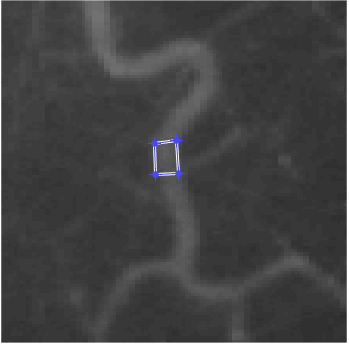
\includegraphics[width=4cm]{figure/vessel2init1.png}} 
   & \subfloat[]{\includegraphics[width=4cm]{figure/vessel2lbf1.png}}
    & \subfloat[]{\includegraphics[width=4cm]{figure/vessel2lif1.png}}
     & \subfloat[]{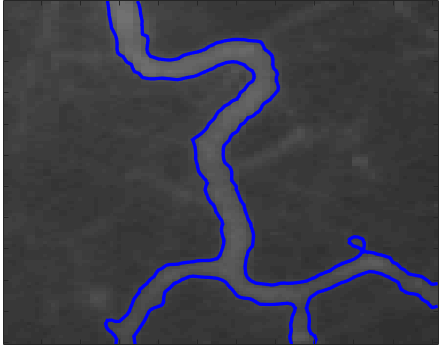
\includegraphics[width=4cm]{figure/vessel2GLIF1.png}} \\
     \subfloat[]{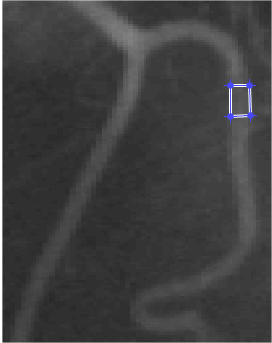
\includegraphics[width=4cm]{figure/vessel3init1.png}} 
   & \subfloat[]{\includegraphics[width=4cm]{figure/vessel3lbf1.png}}
    & \subfloat[]{\includegraphics[width=4cm]{figure/vessel3lif1.png}}
     & \subfloat[]{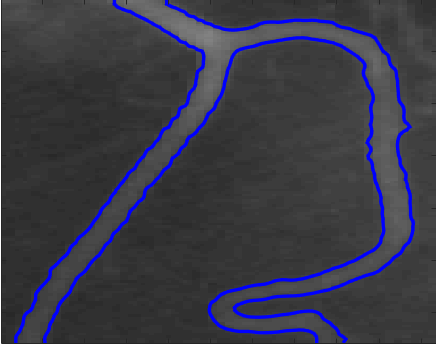
\includegraphics[width=4cm]{figure/vessel3GLIF1.png}}\\
     \subfloat[]{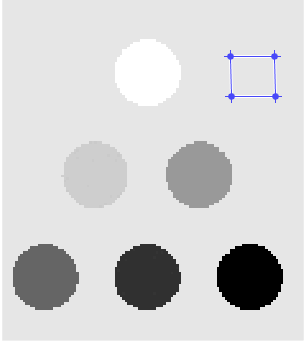
\includegraphics[width=4cm]{figure/3cinit1.png}} 
   & \subfloat[]{\includegraphics[width=4cm]{figure/3clbf1.png}}
    & \subfloat[]{\includegraphics[width=4cm]{figure/3clif1.png}}
     & \subfloat[]{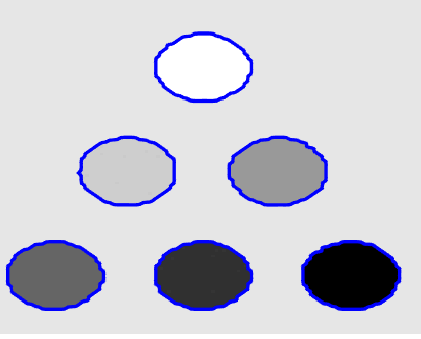
\includegraphics[width=4cm]{figure/3cGLIF1.png}}\\
      \subfloat[]{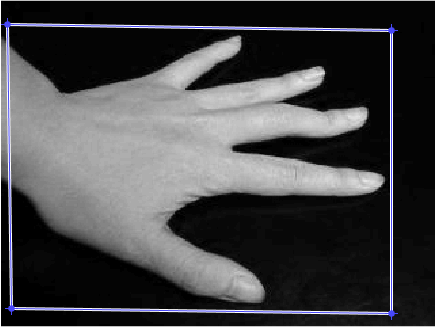
\includegraphics[width=4cm]{figure/bantayinit1.png}} 
   & \subfloat[]{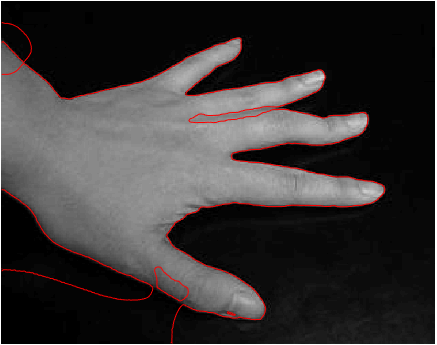
\includegraphics[width=4cm]{figure/bantaylbf1.png}}
    & \subfloat[]{\includegraphics[width=4cm]{figure/bantaylif1.png}}
     & \subfloat[]{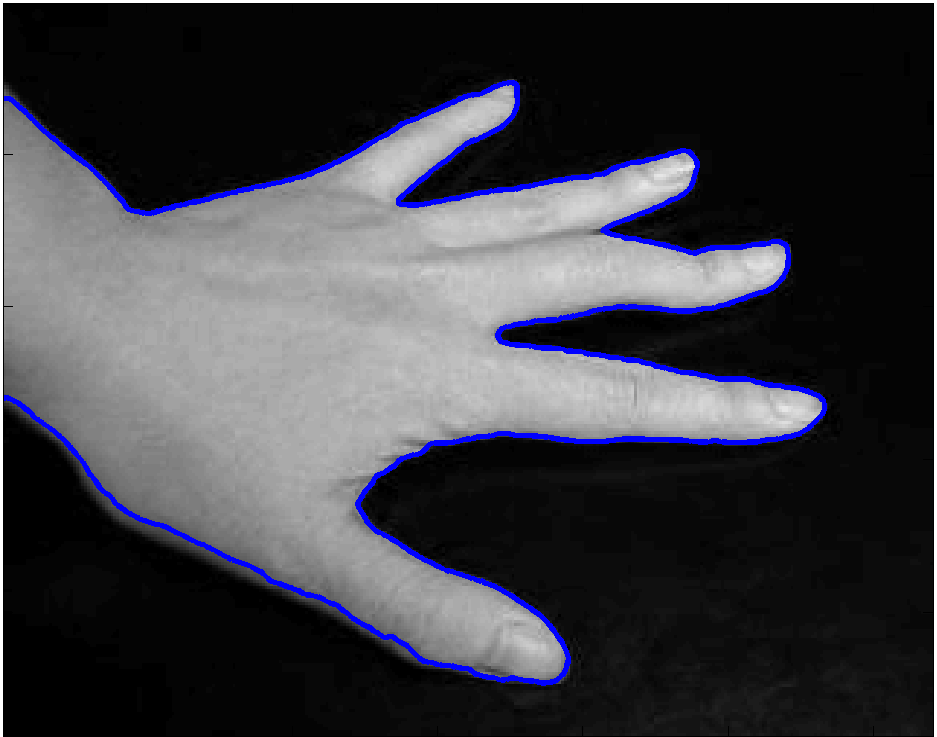
\includegraphics[width=4cm]{figure/bantayGLIF1.png}}                
   \end{tabular}


\caption{Kết quả của mô hình GLIF so với các mô hình LBF và LIF. Ảnh a, e, i, m là đường cong khởi tạo ban đầu. Ảnh b,f,j,n là kết quả với mô hình LBF, ảnh c, g, k, o là kết quả với mô hình LIF. Ảnh d, h, l, p là kết quả với mô hình GLIF }\label{foo}
\end{figure}
Kết quả hình $(3.9)$ cho thấy mô hình GLIF xử lý tốt với cả ảnh đồng nhất cường độ và ảnh không đồng nhất cường độ. Đặc biệt  kết quả thực nghiệm cho thấy mô hình GLIF hoạt động được trong trường hợp $\Delta t$ lớn hơn so với các mô hình LBF và LIF trong khi vẫn đưa ra kết quả chấp nhận được. Điều này giúp tăng tốc độ chạy thuật toán. Hình $(3.12)$ là kết quả minh chứng cho điều này:
\begin{figure}[]
\def\tabularxcolumn#1{m{#1}}
%
\begin{tabular}{ccc}
    \subfloat[]{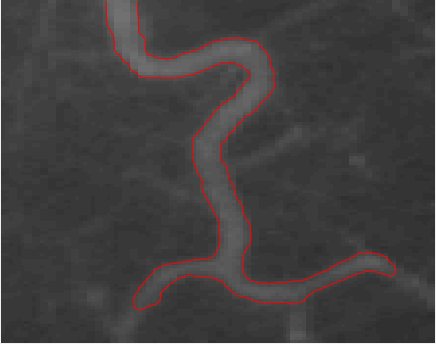
\includegraphics[width=4cm]{figure/vessel2lbf2.png}}
    & \subfloat[]{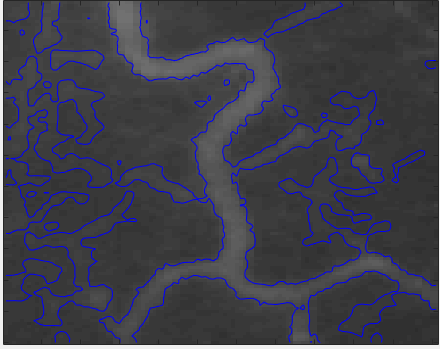
\includegraphics[width=4cm]{figure/vessel2lif2.png}}
     & \subfloat[]{\includegraphics[width=4cm]{figure/vessel2GLIF2.png}} \\
    \subfloat[]{\includegraphics[width=4cm]{figure/vessel3lbf2.png}}
    & \subfloat[]{\includegraphics[width=4cm]{figure/vessel3lif2.png}}
     & \subfloat[]{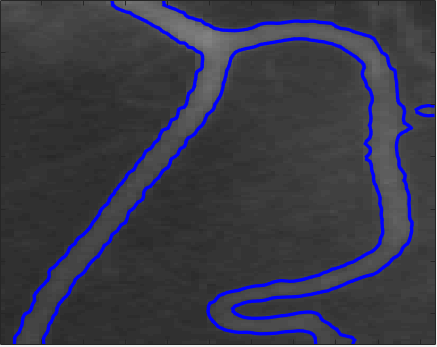
\includegraphics[width=4cm]{figure/vessel3GLIF2.png}}               
   \end{tabular}


\caption{Kết quả của mô hình GLIF so với các mô hình LBF và LIF với tham số $\Delta t=0.1$. Ảnh a, d là kết quả với mô hình LBF, ảnh b, e là kết quả với mô hình LIF. Ảnh c, f là kết quả với mô hình GLIF }\label{foo}
\end{figure}
\chapter{Áp dụng mô hình GLIF trong theo dõi đối tượng trong video }
\section{Theo dõi đối tượng trong video là gì? Tại sao phải theo dõi đối tượng trong video}
Theo vết đối tượng là một vấn đề quan trọng trong trong lĩnh vực thị giác máy tính. Sự xuất hiện của các máy tính cấu hình mạnh và các camera chất lượng cao và sự cần thiết của việc phân tích video  là điều kiện để thúc đẩy sự phát triển của các thuật toán theo vết. Có 3 bước chính trong phân tích video là: Phát hiện các đối tượng chuyển động trong video, theo vết các đối đó theo từng frame, phân tích vết để phát hiện hành động của đối tượng. Do vậy, theo vết đối tượng phù hợp với: 
\begin{itemize}
\item Nhận dạng dựa trên chuyển động
\item Giám sát tự động, hay là theo dõi một cảnh để phát hiện các hoạt động đáng ngờ hoặc các sự kiện bất thường.
\item Lập chỉ mục video, tạo chú thích tự động và tìm kiếm video trong cơ sở dữ liệu.
\item Tương tác giữa con người và máy tính, hay là nhận diện cử chỉ, theo dõi mắt làm đầu vào cho máy tính. 
\item Theo dõi giao thông, thu thập thống kê dòng phương tiện
\end{itemize}
Ở dạng đơn giản nhất, theo vết có thể được định nghĩa là ước lượng chuyển động của đối tượng trong miền ảnh khi nó chuyển động xung quanh miền ảnh. Một cách khác, người theo dõi thực hiện gán nhãn các đối tượng được theo dõi trong các khung hình của video. Ngoài ra, tùy thuộc vào miền ảnh, việc theo dõi có thể cung cấp các đặc tính của đối tượng như: hình dạng, vị trí, hướng. Việc theo vết đối tượng có thể gặp khó khăn do một số ấn đề như: 
\begin{itemize}
\item Thiếu thông tin do các phép chiếu từ khung cảnh 3D ngoài đời thực vào ảnh 3D
\item Ảnh nhiễu
\item Những chuyển động phức tạp của đối tượng
\item Thay đổi khung cảnh
\item Yêu cầu xử lý thời gian thực
\end{itemize} 
Điều này có thể đơn giản hơn nhờ việc đưa vào các ràng buộc về chuyển động cũng như là bề ngoài củ đối tượng. Ví dụ, hầu hết các thuật toán theo vết đối tượng đều đưa vào ràng buộc tốc độ và gia tốc là hằng số. 

Có nhiều phương pháp theo vết đối tượng được đề xuất. Các hướng này khác nhau ở cách tiếp cận để trả lời các câu hỏi: Đối tượng nào thích hợp để theo dõi? Các đặc tính nào của ảnh có thể sử dụng? Làm sao để mô hình hóa hình dạng, chuyển động của đối tượng trong video? Việc trả lời các câu hỏi này còn tùy thuộc vào hoàn cảnh, điều kiện .
\section{Biểu diễn đối tượng }
Đối tượng có thể được định nghĩa là bất kỳ thứ gì mà người ta quan tâm và muốn phân tích nó. Ví dụ như các phương tiện ở trên đường, người đi bộ trên đường, hay các bong bóng ở trong nước .... Các đối tượng có thể được đại diện bởi hình dạng, đối tượng.... Dưới đây là một số cách dùng để biểu diễn hình dạng đối tượng thường được sử dụng trong  theo vết. 
\begin{itemize}
\item Điểm: Một đối tượng được biểu diễn bởi một tập hợp các điểm. Cách này thường được dùng trong trường hợp đối tượng được theo vết có kích thước nhỏ
\item Các hình dạng cơ bản: Đối tượng được đại diện bởi các đường thằng, tam giác, elips,.... Chuyển động của đối tượng theo cách tiếp cận này được mô hình hóa bằng các dịch chuyển, tuyến tính, hay phép chiếu. Mặc dù cách này phù hợp với việc theo dấu các đối tượng rigrid tuy nhiên nó có thể dùng cho các đối tượng non-rigrid.
\item Đường viền : Đường viền đại diện cho biên của vật. Phần bên trong đường viền được gọi là silhouette của đối tượng. Cách biểu diễn sử dụng đường biên này phù hợp với đối tượng non-rigrid
\item Khớp nối: Một đối tượng sẽ được chia thành các phần khác nhau và được kết nối bởi các khớp nối. Ví dụ với cơ thể người có thể được chia ra làm các phần: thân, chân, tay,  đầu được kết nối bởi các khớp nối. Quan hệ giữa các thành phần được chi phối bởi các mô hình động học.
\end{itemize}
\subsection{Lựa chọn đặc tính để thực hiện theo vết}
Thông thường, để đạt được kết quả như mong muốn, người ta thường chọn thuộc tính đảm bảo được tính duy nhất để đảm bảo đối tượng có thể được phân biệt. Các đặc tính này thường được chọn để phù hợp với cách biểu diễn đối tượng. Ví dụ màu thường được dùng làm đặc tính để tìm vết trong trường hợp đối tượng được biểu diễn bởi biểu đồ histogram. Còn cạnh đối tượng thường được dùng làm đặc tính trong trường hợp biểu diễn đối tượng bằng đường viền. Và thông thường chúng thường trong thực tế chúng thường được kết hợp với nhau để được kết quả cao hơn. Các đặc tính thường được dùng là:
\begin{itemize}

\item Màu sắc của một vật bị ảnh hường bởi các yếu tố  phân bố điện quang của ánh sáng và tính chất phản xạ bề mặt của đối tượng. Không gian màu RGB thường được dùng nhiều trong xử lý ảnh, nó là không gian màu không đồng nhất cảm quan(non perceptually uniform ), hay sự khác biêt về màu trong hệ RGB không tương ứng với sự khác biệt về màu đối với cảm nhận của con người. Ngược lại hệ màu $L^*u^*v, L^*a^*b$ lại là không gian màu đồng nhất cảm quan. Tuy vậy nó lại nhạy cảm với nhiễu. Do  mỗi không gian màu sẽ có một ưu nhược điểm riêng và không thể nói được rằng không gian màu nào được dùng sẽ hiệu quả hơn nên trong thực tế người ta dùng rất nhiều loại không gian màu khác nhau để thực hiện tìm vết
\item Cạnh : Biên của đối tượng thường là nơi có sự thay đổi lớn về cường độ ảnh. Thuộc tính quan trọng của đặc tính này là nó ít nhạy cảm hơn với sự thay đổi về độ sáng hơn là đặc tính màu. 

\item Texture: Texture giống như một độ đo sự biến đổi cường độ trên bề mặt thỏa mãn các thuộc tính. như độ trơn, độ đều. So với màu, texture cần thêm thao tác xử lý để có được đặc tính. 

\end{itemize}
\section{Theo vết đối tượng sử dụng mô hình GLIF}
Thuật toán dừng lại cơ bản là áp dụng mô hình GLIF trong mỗi frame trong video, sử dụng kết quả cuối cùng của một khung hình làm đầu vào cho khung hình sau. Dưới đây là giả code cho mô hình này:
\begin{lstlisting}
Co=initial Contour
for k=1 to n_frame 
{
C_k=GLIF(C{k-1},I_{k});
draw contour on image
output frame
}

\end{lstlisting}
Trong quá trình áp dụng mô hình GLIF cho theo vết đối tượng  , tôi chỉ thực hiện đưa ra kết quả với các video với độ đồng nhất cao trong đối tượng và ngoài đối tượng.  
\section{Kết quả}
Một vấn đề xảy ra là quá trình áp dụng  mô hình này  trong thực tế cho thấy tốc độ còn chậm mặc dù đường biên của đối tượng trong frame trước khá gần với đường biên của đối tượng trong frame sau. Do đó tôi thực hiện thay đổi quá trình khởi tạo lại hàm $\phi$ bằng hàm dấu khoảng cách thành việc khởi tạo lại hàm $\phi$ thành hàm khác với các giá trị bằng $c_0(c_0>0)$ nếu $\phi(x)>0$ và bằng $-c_0$ nếu $\phi(x)<0$ . Kết quả thực nghiệm cho thấy áp dụng việc khởi tạo  tỏ ra hiệu quả hơn nhiều so với việc không khởi tạo lại hàm $\phi$. Hình 4.1 thể hiện kết quả của thuật toán trong khác frame khác nhau của video. Kết quả cho thấy thuật toán hoạt động tốt ngay cả trong trường hợp có sự thay đổi lớn trong các frame hay trong trường hợp biên trong frame sau không giao nhau với biên của đối tượng trong frame trước.
\begin{center}
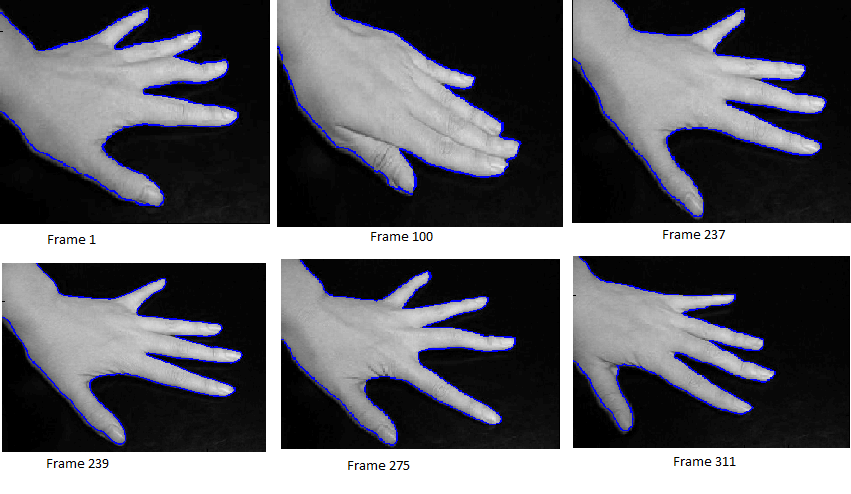
\includegraphics[scale=0.5]{figure/video1.png}
\captionof{figure}{Kết quả trong các frame khác nhau}
\end{center}   
\begin{center}
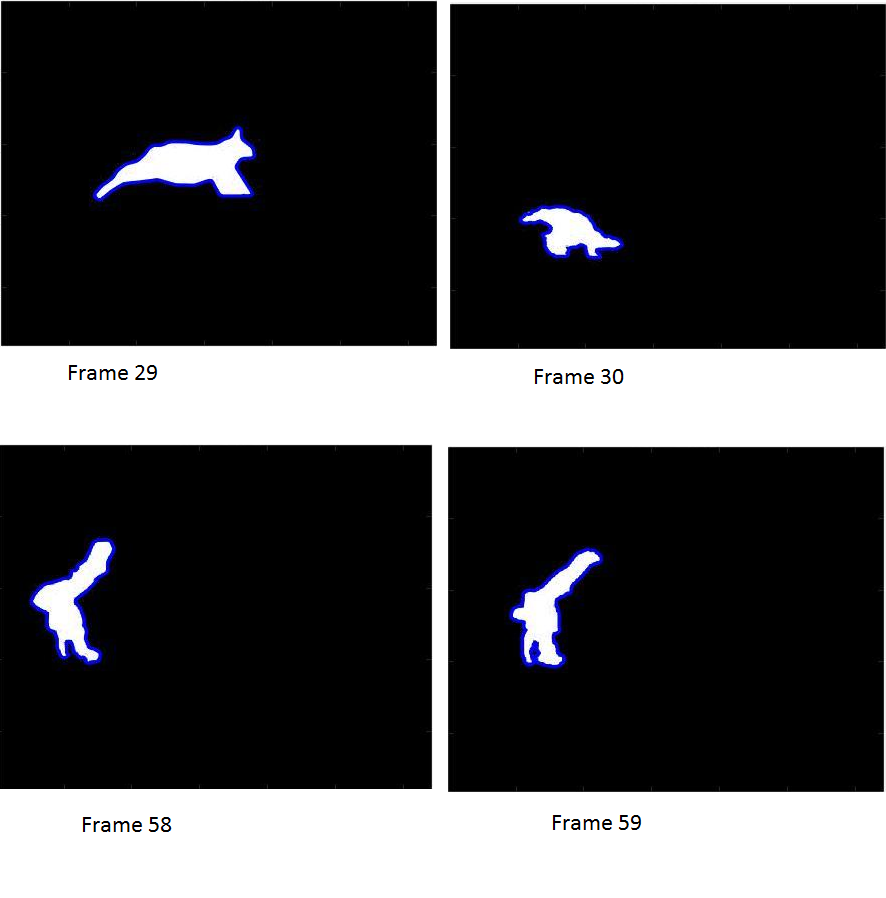
\includegraphics[scale=0.5]{figure/animals.png}
\captionof{figure}{Kết quả trong trong trường hợp có sự thay đổi lớn về vị trí của đối tượng}
\end{center}
\chapter{Áp dụng GLIF trong phân vùng ảnh 3 chiều}
\section{Ảnh ba chiều trong thực tế và một số phương pháp phân vùng}
\subsection{Ảnh ba chiều trong thực tế}
Ngày nay, với sự ra đời của các thiết bị y tế  như máy chụp cắt lớp (CT), máy cộng hưởng từ (MRI) với khả năng cung cấp hình ảnh 3 chiều của các bộ phận trong cơ thể, các bác sĩ đã dễ dàng chuẩn đoán và thực hiện thao tác với các bộ phận trong thực tế hơn nhờ quan sát trên các hình ảnh  3 chiều. Các thiết bị hoạt động theo cơ chế dùng tia X quang chụp cắt lớp các bộ phận theo nhiều hướng khác nhau. Hình ảnh cắt lớp 2 chiều được chụp từ các thiết bị này sau đó sẽ được đưa vào máy tính xử lý để có thể tạo dựng lại hình ảnh 3 chiều. Một bức ảnh 3 chiều gốc có thể coi như là một mảng 3 chiều các voxel. Các voxel này sẽ được đặc trưng bởi một mức xám với giá trị nằm trong khoảng từ 0 đến 65535 trong trường hợp voxel được biểu diễn bởi 16 bit hoặc từ 0 đến 255 trong trường hợp voxel được biểu diễn bởi 8 bit. Một ảnh 3 chiều bình thường cho ra từ các thiết bị sẽ có số lượng voxel tương đối lớn và yêu cầu tính toán nhiều cho các quá trình xử lý trong phân vùng hoặc nhận dạng. 
Một ảnh 3 chiều được định nghĩa trên miền ảnh $\Omega$ như sau: 
\begin{equation}
\begin{split}
&f(x)\in \mathbb{R}\\
&x\in \Omega
\end{split}
\end{equation} 
Trong đó $\Omega$ là không gian rời rạc 3 chiều. Một ảnh đã được phân vùng được định nghĩa trong cùng miền $\Omega$ với ảnh f nhưng lấy giá trị trong không gian nhãn rời rạc. 
\begin{equation}
g(x)\in \mathbb{N}
\end{equation}
Ảnh nhị phân là một trường hợp đặc biệt của định nghĩa này, hàm g nhận giá trị 0 hoặc 1 tương ứng với nền và phần nội dung trong ảnh. 
Việc  phân vùng trong 3 chiều với ảnh y tế ngoài mục đích hiển thị ảnh còn có thể giúp ích rất lớn cho việc chuẩn đoán, điều trị, đánh giá kết quả của các phương pháp điều trị. Ví dụ việc phân vùng được ứng dụngtrong việc đo tỷ lệ giữa thể tích của phần não bị ảnh hưởng do việc điều trị so với tổng thể tích của não, hoặc đơn giản hơn là đo thể tích của não hay các cơ quan khác mà nếu dùng cách khác sẽ tốn rất nhiều thời gian hoặc công sức.

Trong thực tế người ta đã đưa ra rất nhiều phương pháp khác nhau để thực hiện phân vùng với ảnh 3 chiều tùy thuộc vào ứng dụng, loại ảnh sử dụng và nhiều yếu tố khác. Ví dụ như việc phân vùng với phổi sẽ khác với việc phân vùng với đại tràng. Một phương pháp có kết quả tốt với loại ảnh này nhưng có thể nó lại không hoạt động với ảnh khác. Bên cạnh đó một số tác nhân khác như nhiễu hay các hiệu ứng khối cũng có thể ảnh hưởng đến kết quả phân vùng. Sự ảnh hưởng của đa dạng các yếu tố đã làm phân vùng ảnh trong 3 chiều trở nên khó khăn.
\subsection{Một số kỹ thuật phân vùng ảnh ba chiều}
Các kỹ thuật phân vùng ảnh 3 chiều được chia làm 3 loại chính theo cách tiếp cận phân vùng là:
\begin{itemize}
\item Kỹ thuật cấu trúc
\item Kỹ thuật ngẫu nhiên
\item Kỹ thuật kết hợp
\end{itemize}
Kỹ thuật cấu trúc thực hiện sử dụng thông tin về cấu trúc của vùng để thực hiện phân vùng. Kỹ thuật ngẫu nhiên áp dụng trực tiếp trên từng voxel mà không sử dụng các thông tin về cấu trúc vùng. Thông tin cục bộ của từng voxel sẽ phục vụ cho việc xác định voxel có thuộc miền đang xét hay không. Kỹ thuật kết hợp thực hiện kết hợp các đặc trưng của các kỹ thuật cấu trúc và ngẫu nhiên để thực hiện cho việc phân vùng.
\section{Kết quả mô hình GLIF cho ảnh ba chiều}
Có hai hướng tiếp cận chính trong phân vùng ảnh 3 chiều là thực hiện xử lý trên từng lát ảnh hoặc xử lý trực tiếp trên ba chiều. Việc phân vùng theo từng lát ảnh về cơ bản không sử dụng được thông tin kết nối giữa các điểm ảnh giữa các lát ảnh cạnh nhau. Trong phần này tôi thực hiện tiếp cận theo cách thứ 2 tức là thuật toán sẽ thực hiện xử lý trực tiếp trên ảnh 3 chiều thay vì xử lý trên từng lát ảnh. Việc sử dụng hướng này sẽ giúp sử dụng được thông tin kết nối giữa các lát ảnh với nhau.
Để có thể áp dụng mô hình GLIF cho ảnh ba chiều thay vì xuất phát từ một đường cong khởi tạo ban đầu ta thực hiện xuất phát từ một mặt khởi tạo ban đầu. Các hàm năng lượng được viết lại trong ba chiều tương tự trong hai chiều. Dưới đây là kết quả phân vùng trong ảnh 3 chiều chạy chiều. HÌnh $(5.1)$, $(5.3)$ là kết qủa quá trình tiến hóa mặt  với các tham số trong thuật toán là $\Delta t=4,\psi=0.3,\mu=0.1 $.HÌnh $(5.2)$,  $(5.4)$ là kết quả trên từng lát ảnh được trích ra từ kết quả đầu ra.
\begin{figure}[]
\def\tabularxcolumn#1{m{#1}}
%
\begin{tabular}{cc}
\subfloat[Mặt khởi tạo ban đầu]{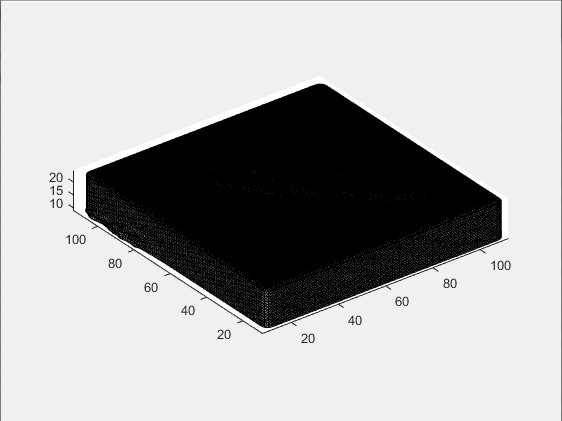
\includegraphics[width=7cm]{figure/lobster1.png}} 
   & \subfloat[Bước lặp 11]{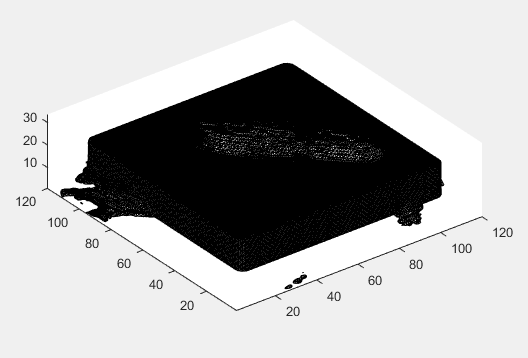
\includegraphics[width=7cm]{figure/lobster11.png}}\\  
    \subfloat[Bước lặp 19]{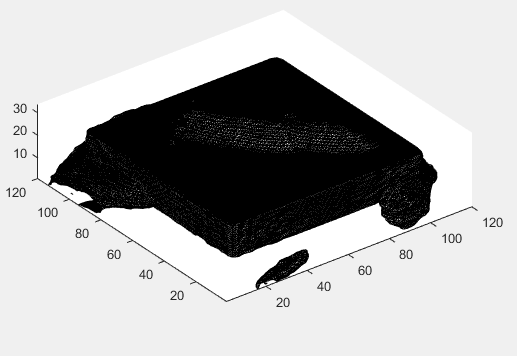
\includegraphics[width=7cm]{figure/lobster19.png}} 
   & \subfloat[Bước lặp 40]{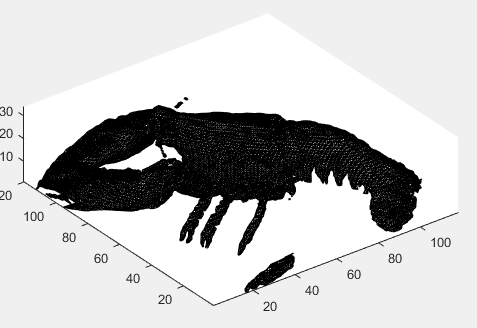
\includegraphics[width=7cm]{figure/lobster40.png}}    
   \end{tabular}


\caption{Kết quả của mô hình GLIF với ảnh chụp cắt lớp một con tôm}\label{foo}
\end{figure}
\begin{center}
\begin{figure}
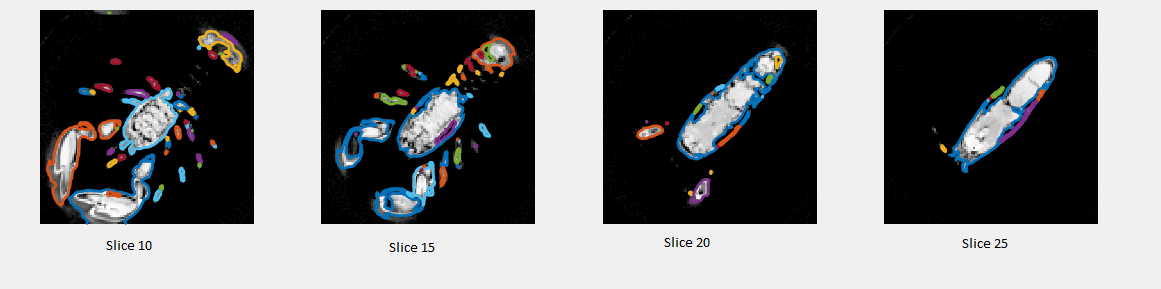
\includegraphics[scale=0.5]{figure/lobsterslice.png}
\caption{Kết quả phân vùng trong các lát ảnh khác nhau}
\end{figure}
\end{center}
Hình $(5.3)$ là kết qủa quá trình tiến hóa mặt được thực hiện trên ảnh chụp cắt lớp não với các tham số trong thuật toán là $\Delta t=0.1,\psi=0.3,\mu=0.1 $.Hình $(5.4)$ là kết trên từng lát ảnh ứng với kết quả đầu ra tương ứng với hình $(5.3)$.
\begin{figure}[]
\def\tabularxcolumn#1{m{#1}}
%
\begin{tabular}{cc}
\subfloat[Mặt khởi tạo ban đầu]{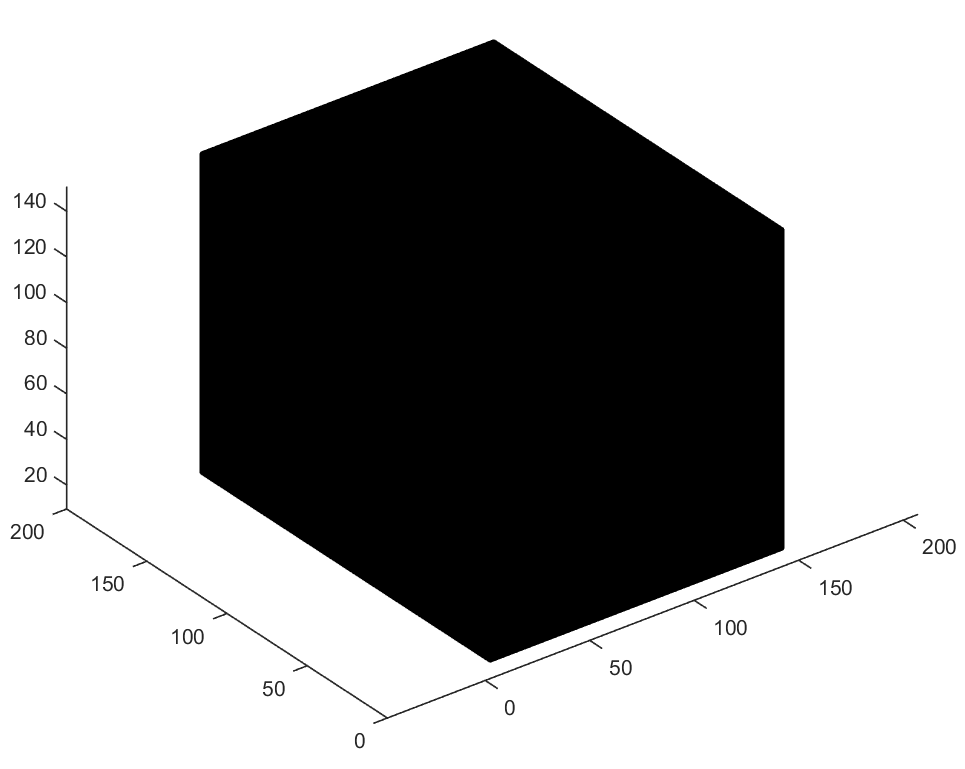
\includegraphics[width=7cm]{figure/braininit1.png}} 
   & \subfloat[Bước lặp 11]{\includegraphics[width=7cm]{figure/brain11.png}}   
   \end{tabular}


\caption{Kết quả của mô hình GLIF với ảnh chụp cắt lớp não người}\label{foo}
\end{figure}
\begin{center}
\begin{figure}
\includegraphics[scale=0.5]{figure/brainslice1.png}
\caption{Kết quả phân vùng hình chụp cắt lớp não trên các lớp ảnh khác nhau}
\end{figure}
\end{center}
\newpage
\begin{center}
\begin{huge}
Kết luận
\end{huge}
\end{center}
1. Kết quả đạt được

Trong quá trình hoàn thành đồ án, tôi đã đạt được các kết quả sau:

- Có được kiến thức cơ bản về xử lý ảnh cũng như bài toán phân vùng.

- Đưa ra được mô hình cải tiến dựa trên các mô hình phân vùng đã được đưa ra.

- Xây dựng được chương trình áp dụng phân vùng trong xử lý video và ảnh 3D.\\
2. Hạn chế

- Phần lý thuyết trình bày lý thuyết chưa chi tiết vào các bước thực hiện từng hướng phân vùng

- Phần xử lý video chỉ dừng lại ở việc xử lý video tĩnh và chưa thực hiện được xử lý thời gian thực do hạn chế về tốc độ tính toán.\\
3. Hướng phát triển:

- Tiếp tục cải tiến thuật toán để có thể xử lý video trong thời gian thực

- Tìm hiểu xây dựng phương pháp tự động chọn biên ban đầu phù hợp với ảnh đầu vào.
\newpage
\begin{thebibliography}{7}
\bibitem{latex}Chunming Li, Chiu-Yen Kao, John C. Gore, and Zhaohua Ding, Implicit Active Contours Driven by Local Binary Fitting Energy,  IEEE Conference on Computer Vision and Pattern Recognition, 2007.
\bibitem{latex}Vaclav Uher and Radim Burget, Automatic 3D Segmentation of Human Brain
Images Using Data-mining Techniques, 35th International Conference on Telecommunications and Signal Processing, 2012.
\bibitem{latex}Kaihua Zhang, Huihui Song, Lei Zhang, Active contours driven by local image fitting energy, Pattern Recognition, 2010.
\bibitem{latex}Mark Moelich, Tony Chan, Tracking objects with the Chan-Vese Algorithm , Mathematics Department, UCLA, 2003.
\bibitem{latex}Olivier Rousseau, Yves Bourgault,  Heart segmentation with an iterative Chan-Vese
algorithm, University of Ottawa, Ontario , 2009.
\bibitem{latex}Rafael C. Gonzalez, Richard E. Woods, \textsl{Digital Image Processing}, 3rd edition, Pearson Education, Inc, USA, 2008.
\bibitem{latex}Sarang Lakare,  3D Segmentation Techniques for Medical Volumes, Research Proficiency, Department of Computer Science State University of New York at Stony Brook, 2000.
\bibitem{latex}Tony Chan, Luminita Vese, An Active Contour Model without Edges, IEEE Trans. Image
Processing, Vol. 10, No. 2,  2001.
\bibitem{latex}Y. Ted Wu, Image segmentation: The first step in 3-D imaging, Able Software Corp,  1999.
\bibitem{latex}Lương Mạnh Bá, Nguyễn Thanh Thủy, \textsl{Nhập môn xử lý ảnh số},Nhà xuất bản Khoa học và Kỹ thuật, Hà Nội, 2006.
\bibitem{latex}Nguyễn Văn Thành, \textsl{Phân tích một số phương pháp phân đoạn ảnh có giám sát}, Đồng Nai 2013.

\end{thebibliography}
\thispagestyle{empty}
%Phương trình Navier-Stokes không nén thường được sử dụng để mô hình hóa nhiều hiện tượng vật lý quan trọng trong thực tế, như dòng chảy của máu, dòng chảy trong các đường ống, dòng không khí chuyển động xung quanh cánh máy bay, các hiện tượng truyền nhiệt và thời tiết. Trong những thập kỷ qua, việc phát triển và phân tích các phương pháp số cho các bài toán về dòng chảy Stokes và Navier-Stokes không nén đã đạt được nhiều tiến bộ to lớn, thể hiện qua những nghiên cứu và nguồn tài liệu dồi dào về đề tài này. Nhiều gói phần mềm mã nguồn mở cũng như thương mại đã được phát triển và có thể được sử dụng như những "hộp đen" để giải quyết một lớp lớn các bài toán trong công nghiệp. Tuy nhiên, các bài toán về phương trình Navier-Stokes vẫn tiếp tục đặt ra những yêu cầu và thách thức lớn lao cho các nghiên cứu trong tương lai, nhằm phát triển và hoàn thiện hơn nữa các phương pháp giải số cho lớp bài toán này.\\
%Ta biết rằng, việc xấp xỉ tuyến tính cho cả vận tốc và áp suất trong bài toán Navier-Stokes sẽ dẫn đến một phép rời rạc hóa không ổn định, do không thỏa mãn điều kiện Babuska-Brezzi. Một phương pháp xấp xỉ rất phổ biến đối với bài toán Stokes được đề xuất bởi Arnold, Brezzi and Fortin \cite{ABF84}. Phương pháp này đề xuất xây dựng không gian các hàm "bubble", hay còn được biết đến là các phần tử Mini (Mini-element). Một tài liệu tham khảo chuẩn tắc về các phương pháp phần tử hữu hạn hỗn hợp là cuốn sách của Brezzi và Fortin \cite{BF91}. Giải pháp cho các kết hợp không hợp lý như trên là bổ sung các thành phần ổn định \cite{BF08,BH08}. Nói cách khác, một nhược điểm của quá trình giải số cho bài toán Navier-Stokes là tính ổn định của thành phần đối lưu trong phương trình động lực. Nhiều tác giả đã sử dụng kỹ thuật "upwinding" để xử lý thành phần hyperbolic này, chẳng hạn như \cite{RR99} dựa trên lược đồ phân phối thặng dư PSI (positive stream invariant), \cite{Mau95} đề xuất phương pháp Arbitrary Lagrangian Eulerian (ALE).\\
%Các nghiên cứu trong đồ án này nhằm mục đích sử dụng các lợi thế của phép xấp xỉ liên tục Galerkin (phần tử hữu hạn Taylor-Hood) \cite{Qua09} và phương pháp đặc trưng cho thành phần không tuyến tính. Xấp xỉ này cho phép ta rời rạc hóa thời gian và tránh những hạn chế về mặt lý thuyết của CFL (Courant-Friedrichs-Levy) trên mỗi bước thời gian (\cite{PLT92} đề xuất cách lựa chọn bước thời gian phù hợp là $\De t \approx 1.5h$).
%Hơn nữa, nếu quỹ đạo đặc trưng được tính toán chính xác thì kết quả của lược đồ giải số là {\it ổn định không điều kiện}.
%%-----------------
%\chapter{Nội dung nghiên cứu}
%\section{Phương trình Navier-Stokes không nén}
%Trong đồ án này, ta xét các bài toán Navier-Stokes không nén phụ thuộc thời gian có dạng:
%\begin{equation}\label{eq:NS1}
%\begin{cases}
% 	\rho\left(\dfrac{\pa{\ve{u}}}{\pa t} + (\ve{u} \cdot \na) \ve{u}\right)-\mu \Delta \ve{u} +\na p &= \rho\ve{f},\quad (\ve{x}, t) \in  \Om\times [0,T]\\
%	\qquad \qquad \qquad \qquad \qquad \qquad \text{div} \ve{u}&=0, \,\,\, \quad (\ve{x}, t) \in  \Om\times [0,T],
%\end{cases}
%\end{equation}
%trong đó, $\Om$ là miền bị chặn trong không gian $\R^d (d=2,3)$ và có biên liên tục Lipschitz $\pa\Om$, $\ve{u} = \ve{u}(\ve{x}, t) \in \R^d$ là vận tốc của dòng chảy ở vị trí $\ve{x}$ tại thời điểm $t$, $p = p(\ve{x}, t) \in \R$ là áp suất dòng chảy, $\ve{f} = \ve{f}(\ve{x}, t) \in \R^d$ là lực tác động từ bên ngoài, $\mu$ là hệ số nhớt và $\rho$ là hệ số mật độ.\\
%Phương trình thứ nhất của hệ \eqref{eq:NS1} biểu diễn nguyên lý bảo toàn động lượng, trong khi phương trình thứ hai thể hiện đặc tính bảo toàn khối lượng của dòng chảy không nén.\\
%Đặt $\nu = {\mu}/{\rho}, p={p}/{\rho}$, ta thu được phương trình Navier-Stokes không nén có dạng đơn giản như sau:
%\begin{equation}\label{eq:NS2}
%\begin{cases}
% \left(\dfrac{\partial{\ve{u}}}{\partial t}+(\ve{u} \cdot \nabla) \ve{u}\right)-\nu \Delta \ve{u} +\nabla p&= \ve{f},\quad (\ve{x}, t) \in  \Om\times [0,T]\\
%\qquad \qquad \qquad \qquad \qquad \qquad \text{div} \ve{u}&=0, \quad (\ve{x}, t) \in  \Om\times [0,T],
%\end{cases}
%\end{equation}
%trong đó, $\nu$ thể hiện hằng số nhớt {\it động học} của chất lỏng.\\
%Cho $L$ là độ dài đặc trưng của dòng chảy. Khi đó, ta định nghĩa số Reynolds:
%\begin{equation}
%Re = \frac{|\ve{u}|.L}{\nu}
%\end{equation} 
%Số Reynolds thể hiện tỉ lệ giữa lực quán tính và lực nhớt. Khi giá trị của $\nu$ lớn, lực nhớt chiếm ưu thế vượt trội, do đó thành phần đối lưu trong phương trình Navier-Stokes có thể bỏ qua. Điều này dẫn đến việc xét phương trình Stokes không dừng sau:
%\begin{equation}\label{eq:S}
%\begin{cases}
% \dfrac{\partial{\ve{u}}}{\partial t}-\nu \Delta \ve{u} +\nabla p&= \ve{f}, \quad (\ve{x}, t) \in \Om\times [0,T]\\
%\qquad \qquad \qquad \text{div} \ve{u}&=0,\quad (\ve{x}, t) \in  \Om\times [0,T] 
%\end{cases}
%\end{equation}
%Để đảm bảo tính đặt chỉnh của bài toán, hệ phương trình \eqref{eq:NS2} cần bổ sung các điều kiện biên thích hợp (Dirichlet, Neumann, slip,...). Đồng thời, các điều kiện biên này cũng cần tương thích với các điều kiện ban đầu, i.e. $\ve{u}(\ve{x},0)=\ve{u}_0(\ve{x}), \, \text{div}\ve{u}_0=0$.
%\section{Phương pháp đặc trưng}
%Trong phần này, ta sẽ tập trung nghiên cứu phương pháp rời rạc hóa thời gian cho phương trình Navier-Stokes bằng phương pháp đặc trưng bậc nhất. Phương pháp này, còn được biết với tên gọi phương pháp Lagrange-Galerkin được giới thiệu đầu tiên bởi Benque \cite{BIK+80}.\\
%Kí hiệu $\ve{X}(\ve{x},s;t)$ là đường cong đặc trưng kết hợp với trường vận tốc $\ve{u}$, là nghiệm của hệ phương trình vi phân thường:
%\begin{equation} \label{eq:ODE1}
%\begin{cases} 
%\dfrac{d\ve{X}(\ve{x},s;t)}{dt}&=\ve{u}(\ve{X}(\ve{x},s;t),t)\\
%\ve{X}(\ve{x},s;s)&=\ve{x},
%\end{cases}
%\end{equation}
%trong đó, điểm $\ve{X}(\ve{x},s;t)$ thể hiện vị trí của dòng chảy tại thời điểm $t$, khi biết tại thời điểm $s$ nó đạt tại vị trí $\ve{x}$.\\
%Lấy đạo hàm trường vận tốc $\ve{u}$ theo đường cong đặc trưng, ta thu được:
%\begin{equation}
%\begin{aligned}
%\dfrac{d\ve{u}(\ve{X}(\ve{x},s;t), t)}{dt} &= \dfrac{\pa\ve{u}}{\pa t} + \na \ve{u}\dfrac{d\ve{X}(\ve{x},s;t)}{dt} = \dfrac{\pa\ve{u}}{\pa t} + \na \ve{u}.\ve{u}(\ve{X}(\ve{x},s;t), t)\\
%&= \dfrac{\pa\ve{u}}{\pa t} + \left(\ve{u}.\na\right)\ve{u}
%\end{aligned}
%\end{equation}
%Phương trình thứ nhất của hệ \eqref{eq:NS2} được viết lại dưới dạng:
%\begin{equation}\label{eq:NS3}
%\dfrac{d{\ve{u}(\ve{X}(\ve{x},s;t),t)}}{dt}-\nu \Delta \ve{u} +\nabla p=\ve{f}
%\end{equation}
%Do đó, việc tính toán thành phần đối lưu phi tuyến trong phương trình Navier-Stokes có thể đưa về bài toán tìm vị trí đặc trưng $\ve{X}(\ve{x},s;t)$, i.e. vị trí của dòng chảy tại thời điểm trước đó.\\
%Giả sử rằng khoảng thời gian $[0,T]$ được chia thành nhiều khoảng bé hơn có cùng độ dài $\De t$ và kí hiệu $t^n=n\De t$. Với mỗi $(t, \ve{x}) \in [t_n, t_{n+1}]\times\overline{\Omega}$, lấy tích phân phương trình \eqref{eq:NS3} theo đường cong đặc trưng, ta thu được:
%\begin{align}\label{eq:NS4}
%\begin{split}
%\ve{u}^{n+1}(\ve{x}) &= \ve{u}^{n}(\ve{X}(\ve{x}, t_{n+1}; t_n))+ \nu\int_{t_n}^{t_{n+1}}\Delta\ve{u}(\ve{X}(\ve{x}, t_{n+1}; t), t) dt\\ 
%&- \int_{t_n}^{t_{n+1}}\na p(\ve{X}(\ve{x}, t_{n+1}; t), t) dt + \int_{t_n}^{t_{n+1}}\ve{f}(\ve{X}(\ve{x}, t_{n+1}; t), t)dt,
%\end{split}
%\end{align}
%trong đó, ta sử dụng các ký hiệu $\ve{u}^n(\cdot) = \ve{u}(\cdot, t_n)$, $p^n(\cdot) = p(\cdot, t_n)$ và $\ve{f}^n(\cdot) = \ve{f}(\cdot, t_n)$. \\
%Các tích phân trong phương trình \eqref{eq:NS4} có thể được ước lượng bằng các lược đồ xấp xỉ. Trong đồ án này, ta rời rạc bước Stokes theo thời gian sử dụng lược đồ $\tta (0\leq \tta \leq 1)$ cho các thành phần của vận tốc và ngoại lực và lược đồ Euler ẩn bậc nhất cho thành phần áp suất. Khi đó ta thu được xấp xỉ:
%\begin{align}\label{eq:NS5}
%\begin{split}
%\ve{u}^{n+1}(\ve{x}) &= \ve{u}^{n}(\ve{X}(\ve{x}, t_{n+1}; t_n))+ \nu\De t\left[\tta\Delta\ve{u}^{n+1}(\ve{x}) + (1-\tta)\Delta\ve{u}^{n}(\ve{X}(\ve{x}, t_{n+1}; t_n))\right]\\ 
%&-  \De t\na p^{n+1}(\ve{X}(\ve{x}, t_{n+1})) + \De t\left[\tta\ve{f}^{n+1}(\ve{x}) + (1-\tta)\ve{f}^{n}(\ve{X}(\ve{x}, t_{n+1};t_n))\right]
%\end{split}
%\end{align}
%Rời rạc bước Stokes theo thời gian có thể được viết lại dưới dạng:
%\begin{align}
%\begin{cases}
%\dfrac{\ve{u}^{n+1}}{\Delta t} - {\tta}.{\nu}\Delta\ve{u}^{n+1} + \na p^{n+1} = \ve{F}^{n+1} &, \, \ve{x} \in  \, \Omega \\
%\na \cdot \ve{u}^{n+1} = 0 &, \, \ve{x} \in \, \Omega
%\end{cases}
%\end{align}
%trong đó $$\ve{F}^{n+1} = \dfrac{\ve{u}^{*n}}{\Delta t} + (1-\tta).{\nu}\Delta\ve{u}^{*n} + \left(\tta\ve{f}^{n+1} +(1-\tta) \ve{f}^{*n}\right),$$ 
%$$\ve{u}^{*n} = \ve{u}^n(\ve{X}(\ve{x}, t_{n+1}; t_n)), \quad \ve{f}^{*n} = \ve{f}^n(\ve{X}(\ve{x}, t_{n+1}; t_n)).$$
%Trường hợp $\tta = 1$, lược đồ xấp xỉ $\tta$ được gọi là {\it lược đồ Euler ẩn bậc nhất}. Trường hợp khác khi $\tta = 1/2$, lược đồ $\tta$ trở thành {\it phương pháp Crank-Nicolson bậc hai}.\\
%Như vậy, tại mỗi bước thời gian, việc tìm nghiệm của bài toán Navier-Stokes sẽ được đưa về giải quyết hai bài toán: bài toán Stokes không dừng và bài toán tìm nghiệm tại bước thời gian trước đó theo đường cong đặc trưng của trường vận tốc $\ve{u}$. Phương pháp rời rạc hóa thời gian cho phương trình Navier-Stokes được chia thành hai bước:
%\begin{itemize}
%\item[i] Giải bài toán vi phân thường \eqref{eq:ODE1} trong khoảng thời gian $[t_n, t_{n+1}]$.
%\item[ii] Giải phương trình Stokes tổng quát được định nghĩa bởi hệ:
%\begin{equation}
%\begin{cases}\label{Stokes}
%\alpha \ve{u} - \beta\Delta\ve{u} + \na p = \ve{F}, & \ve{x} \in\,  \Omega\\
%\na \cdot \ve{u} = 0, &\ve{x}\in \, \Omega,
%\end{cases}
%\end{equation}
%trong đó $\alpha$ ký hiệu cho $\dfrac{1}{\Delta t}$ và $\beta = \tta{\nu}$.
%\end{itemize}
%
%\section{Dạng biến phân của phương trình Navier-Stokes}
%Như đã thảo luận trong phần trước, tại mỗi bước thời gian, ta phải giải một bài toán Stokes không dừng \eqref{Stokes}. Cách giải số cho bài toán này bằng phương pháp phần tử hữu hạn sẽ dẫn đến một công thức biến phân.\\
%Đầu tiên, ta giới thiệu các không gian Sobolev sau:
%\begin{align}
%&H_0^1(\Omega)^d=\{\ve{v}\in H^1(\Omega)^d: \ve{v}|_{\pa \Om}=0\} \label{eq:V}\\ 
%&L_0^2(\Omega)=\{q\in L^2(\Omega) :\int_\Omega q=0\}\label{eq:M}
%\end{align}
%Ký hiệu $V$ và $M$ là các không gian hàm cho vận tốc và áp suất tương ứng. Ta xét dạng biến phân của bài toán Stokes tổng quát trong trường hợp điều kiện biên Dirichlet thuần nhất, i.e $\ve{u}|_{ \pa \Om}=0$. Khi đó, $V$ sẽ được chọn trùng với $H^1_0(\Omega)^d$ và $M=L^2_0(\Omega)$ cho áp suất.\\
%Cho trước $\ve{v} \in V$. Nhân $\ve{v}$ vào hai vế của phương trình thứ nhất trong hệ \eqref{Stokes} rồi lấy tích phân, ta được:
%\begin{equation}\label{Stokes1}
%\alpha \int_\Om {\ve{u}}.{\ve{v}}dx - \beta \int_\Om{ \Delta \ve{u}.\ve{v}} dx + \int_\Om \na p.\ve{v}dx = \int_\Omega\ve{F}.{\ve{v}}dx
%\end{equation}
%Từ công thức Green, ta có:
%\begin{align}\notag
%- \beta\int_{\Omega} \Delta \ve{u} \ve{v} dx 
%&=  \beta \int_{\Omega}\nabla \ve{u}: \nabla \ve{v}dx - \beta \int_{\partial{\Omega} } \nabla \ve{u} \ve{n}.\ve{v}ds \notag\\
%\int_{\Omega} \nabla p.\ve{v}dx&= -\int_{\Omega} p\text{div}\ve{v}dx + \int_{\partial{\Omega} } p\ve{n}.\ve{v}ds \notag
%\end{align}
%Thay các đẳng thức này vào \eqref{Stokes1}, ta được phương trình sau:
%\begin{align}
%\alpha \int_\Om {\ve{u}} .{\ve{v}}dx+ \beta \int_\Om{\nabla \ve{u}: \nabla\ve{v}} dx-\int_\Om p\text{div}\ve{v}dx&= \int_\Om \ve{F}.{\ve{v}}dx +\int_{\partial{\Omega} } (\beta  \nabla \ve{u}-pI_d) \ve{n}.\ve{v}ds\label{eq:NSv}
%\end{align}
%Do $\ve{v}=0$ trên $\pa \Om$ nên ta có:
%\begin{align} \notag
%\alpha\int_\Om{\ve{u}} .{\ve{v}}dx+ \beta \int_\Om{\nabla \ve{u}: \nabla\ve{v}} dx-\int_\Omega p\text{div}\ve{v}dx&= \int_\Om \ve{F}.{\ve{v}}dx\notag 
%\end{align}
%Chọn hàm thử $q \in M$ và nhân cả hai vế của phương trình thứ hai trong hệ \eqref{Stokes} với $q$ trong không gian $L^2(\Om)$, ta thu được dạng biến phân của bài toán thuần nhất: Cho hàm $\ve{F}\in {H^{-1}(\Om)}^d$, các hằng số dương $\alpha$ và $\beta$; tìm $\ve{u} \in V$ và $p \in M$ là nghiệm của hệ:
%\begin{equation} \label{eq:Var}
%\begin{cases}
%\displaystyle \alpha \int_\Om{\ve{u}} .{\ve{v}}dx+ {\beta\int_\Om \nabla \ve{u}: \nabla\ve{v}} dx-\int_\Om p\text{div}\ve{v}dx
%&= \displaystyle\int_\Om \ve{F}.{\ve{v}}dx, \quad \forall \ve{v} \in V\\ \notag
%\quad\quad\quad\quad\quad\quad\quad\quad\quad\quad\quad\quad\quad\quad\displaystyle\int_\Omega q\text{div}\ve{u}dx &= 0, \quad\quad\,\,\,\quad\quad \forall q \in M
%\end{cases}
%\end{equation} 
%Bài toán này có thể được viết dưới dạng yếu tương đương: Tìm $(\ve{u},p) \in (V \times M)$ thỏa mãn:
%\begin{equation}\label{eq:ab}
%\begin{cases}
%\forall \ve{v}\in V &a(\ve{u},\ve{v}) + b(\ve{v},p) = l(\ve{v})\\
%\forall q\in M  &b(\ve{u},q) \qquad \qquad= 0,
%\end{cases}
%\end{equation}
%trong đó $l(\cdot)$ là dạng tuyến tính liên tục được định nghĩa trên $V$: $$l(\ve{v})=\int_\Om\ve{F}.{\ve{v}}dx$$
%và $a(\ve{u},\ve{v}), b(\ve{v},p)$ là các dạng song tuyến tính liên tục được định nghĩa trên $V\times V$ và $V\times M$ tương ứng:
%\begin{equation}
%\begin{cases}
%a(\ve{u},\ve{v}) &= \alpha \displaystyle\int_\Om {\ve{u}} .{\ve{v}}dx+ \beta\int_\Om{ \nabla \ve{u}: \nabla \ve{v}} dx\\
%b(\ve{v},p) &=  \displaystyle-\int_\Om p\text{div}\ve{v}dx
%\end{cases}
%\end{equation}
%Sự tồn tại và duy nhất nghiệm của dạng yếu của bài toán Stokes tổng quát đã được chứng minh trong nhiều nghiên cứu trước đây (xem \cite{GR86} hoặc \cite{EG04}). Các chứng minh này bao gồm: i. tính elliptic của dạng song tuyến tính $a(.,.)$ là kết quả của bất đẳng thức Friedrichs-Poincare; ii. các không gian hàm của vận tốc và áp suất thỏa mãn điều kiện Babuska-Brezzi, còn được gọi là {\it điều kiện inf-sup} trên dạng song tuyến tính $b(.,.)$, i.e. tồn tại một hằng số dương $C$ thỏa mãn:
%\begin{equation}
%\underset{q\in M}{\text{inf}}\underset{\ve{v}\in V}{\text{sup}} \dfrac{b(\ve{v},q)}{\|\ve{v}\|_1\|q\|_0} \ge C >0,
%\end{equation}
%trong đó, $\|\ve{v}\|_1=\left(\Sigma_{i=1}^{d} {\|{v_i}\|_1}^2\right)^{1/2}$ và $\|.\|_1$, $\|.\|_0$ là các chuẩn trong các không gian  Sobolev $H^1(\Om)$, $L^2(\Om)$ tương ứng.
%\section{Rời rạc hóa không gian}
%Bằng cách sử dụng phép xấp xỉ bởi các phần tử hữu hạn Galerkin, dạng rời rạc hóa theo không gian tương ứng với bài toán \eqref{eq:ab} được viết lại như sau: Tìm $(\ve{u}_h, p_h) \in V_h \times M_h$ thỏa mãn:
%\begin{equation}\label{eq:abh}
%\begin{cases}
%\forall \ve{v}_h\in V_h &a_h(\ve{u}_h,\ve{v}_h) + b_h(\ve{v}_h,p_h) = l_h(\ve{v}_h)\\
%\forall q_h\in M _h &b_h(\ve{u}_h,q_h) \qquad \qquad \qquad= 0,
%\end{cases}
%\end{equation}
%trong đó, $V_h \subset V$ và $M_h \subset M$ là hai họ các không gian con hữu hạn chiều phụ thuộc vào một tham số rời rạc hóa $h$-{\it kích thước phần tử đặc trưng} của một phép tam giác phân $T_h$ trên miền $\Omega$;
%và $a_h(\ve{u}_h,\ve{v}_h)$, $b_h(\ve{v}_h,p_h)$, $l_h(\ve{v}_h)$ được định nghĩa như sau:
%\begin{equation}\label{eq:abl_h}
%\begin{cases}
%\displaystyle a_h(\ve{u}_h,\ve{v}_h) = \sum_{K\in T_h}\alpha\int_K  {\ve{u}_h} .{\ve{v}_h}dx + \displaystyle\sum_{K\in T_h} \beta \int_K{\nabla \ve{u}_h: \nabla \ve{v}_h} dx\\
%\displaystyle b_h(\ve{v}_h,p_h) =  -\sum_{K\in T_h}\int_Kp_h\text{div}\ve{v}_hdx\\
%\displaystyle l_h(\ve{v}_h)= \sum_{K\in T_h}\int_K \ve{F}_h.{\ve{v}_h}dx
%\end{cases}
%\end{equation}
%Bài toán xấp xỉ này cũng yêu cầu các điều kiện tương thích rời rạc, còn được gọi là {\it điều kiện inf-sup rời rạc}, nghĩa là tồn tại một hằng số dương $C_h$ thỏa mãn:
%\begin{equation}\label{eq:inf_sup_h}
%\underset{q_h\in M_h}{\text{inf}}\underset{\ve{v}_h\in V_h}{\text{sup}} \dfrac{b_h(\ve{v}_h,p_h)}{\|\ve{v}_h\|_1\|q_h\|_0} \ge C_h >0
%\end{equation}
%Do đó, ta chọn các hàm đa thức từng phần bậc $k\geq 2$ cho không gian hàm của vận tốc $V_h$ và bậc $k-1$ cho không gian hàm của áp suất $M_h$. Trong thực tế, ta chọn các phần tử hữu hạn từng phần dạng bậc hai $\Pp_2$ cho vận tốc và các phần tử hữu hạn tuyến tính $\Pp_1$ cho áp suất. Đây là cặp phần tử có bậc nhỏ nhất của họ các phần tử Taylor-Hood có dạng $\Pp_k /\Pp_{k-1}, k \geq 2$ (vận tốc liên tục và áp suất liên tục) và thỏa mãn {\it điều kiện cân bằng inf-sup}.
%\section{Hệ phương trình tuyến tính rời rạc}
%Đặt $\{\vp_i\}_{i=1,...,nv}$ và $\{\phi_j\}_{j=1,...,np}$ là họ các hàm cơ sở của các không gian $V_h$ và $M_h$ tương ứng, với $nv=\text{dim}V_h$ và $np=\text{dim}M_h$. Cho trước $\ve{u}_h \in V_h$, $p_h \in M_h$, ta có phân tích:
%\begin{equation}
%\begin{aligned}
%\displaystyle \ve{u_h} &= \sum_{i=1}^{nv}u_i \vp_i, \qquad
%\displaystyle p_h&= \sum_{j=1}^{np}p_j \phi_j
%\end{aligned}
%\end{equation}
%Ta giới thiệu các ma trận hệ số:
%\begin{align} \notag
%A_{i,j} = a_h(\vp_i,\vp_j),\qquad
%B_{i,j}=b_h(\vp_i,\phi_j),\qquad
%F_i=l_h(\vp_i),
%\end{align} 
%trong đó, các ma trận $A,B$ tương ứng với các dạng song tuyến tính $a_h,b_h$ và vector $F$ tương ứng với dạng tuyến tính $l_h$ được định nghĩa trong \eqref{eq:abl_h}.\\
%Ký hiệu các vector $U=(u_i)_{i=1,...,nv}$ và $P=(p_j)_{j=1,...,np}$, bài toán \eqref{eq:abh} tương đương với bài toán giải hệ phương trình tuyến tính sau:
%\begin{equation}\label{eq:matrix}
%\begin{pmatrix}A & B^t \\B & 0\end{pmatrix}
%\begin{pmatrix}U\\P\end{pmatrix} =
%\begin{pmatrix}F\\0\end{pmatrix}
%\end{equation}  
%Hệ \eqref{eq:matrix} là hệ thưa, đối xứng nhưng không xác định và kích thước của nó là dim$V_h$ + dim$M_h$.\\
%Có nhiều phương pháp số đã được đề xuất để giải hệ phương trình tuyến tính  \eqref{eq:matrix}. Một phương pháp cổ điển thường được sử dụng là phương pháp {\it Uzawa} \cite{AHU58}, bằng cách đưa hệ \eqref{eq:matrix} về hai hệ phương trình nhỏ hơn, một cho vận tốc chưa biết $U$ và một cho áp suất $P$. Điều này dẫn đến việc giải hai hệ phương trình sau:
%\begin{equation}
%BA^{-1}B^tP=BA^{-1}F, \qquad AU=F-B^tP.
%\end{equation}
%Chú ý, phương pháp {\it Penalty} có thể được sử dụng để tìm $U$ và $P$ trong hệ phương trình tuyến tính sau:
%\begin{equation}
%\begin{pmatrix}A & B^t \\B & \epsilon I_d\end{pmatrix}
%\begin{pmatrix}U\\P\end{pmatrix} =
%\begin{pmatrix}F\\0\end{pmatrix}
%\end{equation}
%trong đó, $I_d$ là ma trận đơn vị cấp $d = \text{dim}M_h$ và giá trị của $\epsilon$ trong khoảng từ $10^{-6}$ đến $10^{-4}$.\\
%Do đó, tại mỗi bước thời gian, bài toán Stokes tổng quát sẽ dẫn đến việc giải một hoặc nhiều hệ phương trình tuyến tính. Các thí nghiệm của chúng tôi được tiến hành với công cụ Freefem++ (\url{http://www.freefem.org}), dựa trên các thuật toán giải hệ phương trình tuyến tính Conjugate Gradient (CG) và Crout. Các phương pháp này được áp dụng phổ biến trong giải hệ phương trình tuyến tính thưa, xem thêm chi tiết trong \cite{She94,Saa03,YJ07}.
%%%%%%%
%\section{Sự ổn định không điều kiện}
%Trong phần này, ta sẽ chứng minh tính {\it ổn định không điều kiện} của lược đồ giải số đã trình bày ở trên trong trường hợp $\tta \geq 1/2$.\\
%Ký hiệu:
%\begin{align*}
%W &= \left\lbrace \ve{v}\in V: \left(q, \na .\ve{v}\right) = 0, \forall q\in M \right\rbrace,\\
%W_h &= \left\lbrace \ve{v}_h\in V_h: \left(q_h, \na .\ve{v}_h\right) = 0, \forall q_h\in M_h \right\rbrace
%\end{align*}
%Chọn $\ve{v} \in W$, phương trình đầu tiên trong hệ \eqref{eq:Var} có thể được viết lại dưới dạng:
%\begin{equation}
%\begin{aligned} \label{eq:Time1}
%\displaystyle \int_\Om \dfrac{\ve{u}^{n+1}}{\De t} {\ve{v}}dx + \theta\nu \int_\Om{ \nabla \ve{u}^{n+1}: \nabla\ve{v}} dx &=\displaystyle\int_\Om \dfrac{\ve{u}^{*n}}{\De t}{\ve{v}}dx + (1-\theta)\nu\int_\Om{\nabla \ve{u}^{*n}: \nabla\ve{v}}dx\\ 
%&+ \theta \int_\Om {\ve{f}^{n+1}\ve{v}dx} + (1-\theta) \int_\Om {\ve{f}^{*n}\ve{v}dx},\quad \forall \ve{v} \in W
%\end{aligned}
%\end{equation}
%Chọn $\ve{v} = \ve{u}^{n+1}$, ta có:
%\begin{equation}
%\begin{aligned} \label{eq:Time2}
%\displaystyle \int_\Om \left(\ve{u}^{n+1}\right)^2dx  + \theta\nu\De t \int_\Om{ \nabla \ve{u}^{n+1}: \nabla\ve{u}^{n+1}} dx &=(1-\theta)\nu\De t\int_\Om{\nabla \ve{u}^{*n}: \nabla\ve{u}^{n+1}}dx\\ 
%&+ \displaystyle\int_\Om \ve{u}^{*n}{\ve{u}^{n+1}}dx  + \theta\De t \int_\Om {\ve{f}^{n+1}\ve{u}^{n+1}dx}\\
%& + (1-\theta)\De t \int_\Om {\ve{f}^{*n}\ve{u}^{n+1}dx}
%\end{aligned}
%\end{equation}
%Viết lại dưới dạng chuẩn, ta có:
%\begin{equation}
%\begin{aligned}
%\norm{\ve{u}^{n+1}}_0^2 + \theta\nu\De t\norm{\nabla\ve{u}^{n+1}}_0^2 \leq &\left(\norm{\ve{u}^{n}}_0 + \theta\De t \norm{\ve{f}^{n+1}}_0 + (1-\theta)\De t\norm{\ve{f}^n}_0\right)\norm{\ve{u}^{n+1}}_0 \\
%&+(1-\theta)\nu\De t\norm{\nabla\ve{u}^n}_0\norm{\nabla\ve{u}^{n+1}}_0
%\end{aligned}
%\end{equation}
%Do $\tta \geq 1/2$ nên $1-\tta \leq \tta$. Do đó:
%\begin{equation}
%\begin{aligned}
%\norm{\ve{u}^{n+1}}_0^2 + \theta\nu\De t\norm{\nabla\ve{u}^{n+1}}_0^2 \leq &\left(\norm{\ve{u}^{n}}_0 + \theta\De t \norm{\ve{f}^{n+1}}_0 + (1-\theta)\De t\norm{\ve{f}^n}_0\right).\\
%&\left(\norm{\ve{u}^{n+1}}_0^2 + \theta\nu\De t\norm{\nabla\ve{u}^{n+1}}_0^2\right)^{1/2} \\
%&+ \sqrt{\theta\nu\De t} \norm{\nabla\ve{u}^n}_0.\left(\norm{\ve{u}^{n+1}}_0^2 + \theta\nu\De t\norm{\nabla\ve{u}^{n+1}}_0^2\right)^{1/2}
%\end{aligned}
%\end{equation}
%Suy ra:
%\begin{equation}
%\begin{aligned}
%\left(\norm{\ve{u}^{n+1}}_0^2 + \theta\nu\De t\norm{\nabla\ve{u}^{n+1}}_0^2\right)^{1/2} \leq & \norm{\ve{u}^{n}}_0 + \theta\De t \norm{\ve{f}^{n+1}}_0 + (1-\theta)\De t\norm{\ve{f}^n}_0\\
%&+ \sqrt{\theta\nu\De t} \norm{\nabla\ve{u}^n}_0
%\end{aligned}
%\end{equation}
%Theo bất đẳng thức Cauchy-Schwarz, ta có (xem thêm phần phụ lục):
%\begin{equation}
%\norm{\ve{u}^{n}}_0 + \sqrt{\theta\nu\De t} \norm{\nabla\ve{u}^n}_0 \leq \sqrt{2}.\left(\norm{\ve{u}^{n}}_0^2 + \theta\nu\De t\norm{\nabla\ve{u}^{n}}_0^2\right)^{1/2}
%\end{equation}
%Như vậy, với $\theta \geq 1/2$:
%\begin{equation}
%\begin{aligned}
%\left(\norm{\ve{u}^{n+1}}_0^2 + \theta\nu\De t\norm{\nabla\ve{u}^{n+1}}_0^2\right)^{1/2} \leq &\theta\De t \norm{\ve{f}^{n+1}}_0 + (1-\theta)\De t\norm{\ve{f}^n}_0\\
%& + \sqrt{2} \left(\norm{\ve{u}^{n}}_0^2 + \theta\nu\De t\norm{\nabla\ve{u}^{n}}_0^2\right)^{1/2}
%\end{aligned}
%\end{equation}
%Bất đẳng thức này thể hiện tính {\it ổn định không điều kiện} của phương pháp giải số. Đặc biệt, trong trường hợp cụ thể, với {\it lược đồ Euler ẩn}, tính {\it ổn định không điều kiện} được biểu diễn qua bất đẳng thức:
%\begin{equation}
%\begin{aligned}
%\left(\norm{\ve{u}^{n+1}}_0^2 + \nu\De t\norm{\nabla\ve{u}^{n+1}}_0^2\right)^{1/2} \leq \De t \norm{\ve{f}^{n+1}}_0 + \left(\norm{\ve{u}^{n}}_0^2 + \nu\De t\norm{\nabla\ve{u}^{n}}_0^2\right)^{1/2}
%\end{aligned}
%\end{equation}

%
%\subsection{The error estimate}
%To simplify, we consider \textit{implicit Euler method}, that mean $\theta = 1$. We call in our problem, the exact solution at the time $t^{n+1}$ is denoted by $\ve{u}^{n+1}$ is solution of equations \eqref{eq:Time1} with:
%\begin{equation}
%\begin{aligned} \label{eq:Err1}
%\displaystyle \int_\Om \dfrac{\ve{u}^{n+1}}{\De t} .{\ve{v}}dx + \nu \int_\Om{ \nabla \ve{u}^{n+1}: \nabla\ve{v}} dx-\int_\Om p^{n+1}\text{div}\ve{v}dx = \displaystyle\int_\Om \dfrac{\ve{u}^{*n}}{\De t}.{\ve{v}}dx  + \int_\Om {\ve{f}^{n+1}.\ve{v}dx}, \quad \forall\ve{v}\in V
%\end{aligned}
%\end{equation}
%while the approximate solution at the time $t^{n+1}$ denoted $\ve{u}_h^{n+1}$ is solution of equation:
%\begin{equation}
%\begin{aligned} \label{eq:Err2}
%\displaystyle \int_\Om \dfrac{\ve{u}_h^{n+1}}{\De t} {\ve{v}_h}dx + \nu \int_\Om{ \nabla \ve{u}_h^{n+1}: \nabla\ve{v}_h} dx-\int_\Om p_h^{n+1}\text{div}\ve{v}_hdx = \displaystyle\int_\Om \dfrac{\ve{u}_h^{n}(\tilde{\ve{X}}_h^n)}{\De t}{\ve{v}_h}dx + \int_\Om {\ve{f}_h^{n+1}\ve{v}_hdx}, \forall\ve{v}_h\in V_h
%\end{aligned}
%\end{equation}
%Denote
%\begin{equation*}
%\ve{{\delta}}^{n+1} = \ve{u}_h^{n+1} - \ve{u}^{n+1}
%\end{equation*}
%Choose test function $\ve{v} = \ve{v}_h$ in $W_h$ for the equation \eqref{eq:Err1} and subtraction of equation \eqref{eq:Err2}, we obtain:
%\begin{equation}\label{eq:Err3}
%\begin{aligned}
%\left(\ve{\delta}^{n+1}, \ve{v}_h \right) + \nu\De t\left(\ve{\na\delta}^{n+1}, \ve{\na v}_h \right) = \De t\left(\ve{f}_h^{n+1} - \ve{f}^{n+1}, \ve{\na v}_h \right) + \left(\ve{\delta}^{n}(\tilde{\ve{X}}^n_h), \ve{v}_h \right) + \left(\ve{u}^n(\tilde{\ve{X}}_h^n) - \ve{u}^n(\ve{X}^n) ,\ve{v}_h\right)
%\end{aligned}
%\end{equation}
%where the second term in right side is subtracted and by $\left(\ve{u}^n(\tilde{\ve{X}}_h^n),\ve{v}_h\right)$.\\
%As in \cite{Pir82} we define $\ve{\eta}^{n+1}$ by
%\begin{equation}\label{eq:Err4}
%\left(\ve{\eta}^{n+1}, \ve{v}_h\right) + \nu\De t\left(\na\ve{\eta}^{n+1}, \na\ve{v}_h\right) = \left(\ve{\eta}^{n+1}, \ve{v}_h\right) + \nu\De t\left(\na\ve{\delta}^{n+1}, \na\ve{v}_h\right), \forall \ve{v}_h \in W_h
%\end{equation}
%then
%\begin{equation}\label{eq:Err5}
%\ve{\eta}^{n+1} = \ve{\delta}^{n+1} + \left(\ve{u}^{n+1}-\Pi\ve{u}^{n+1}\right),
%\end{equation}
%where $\Pi$ is the projector on $V_h$ with respect to the norm
%\begin{equation*}
%\left(\norm{.}_0^2 + \nu\De t\norm{\na .}_0^2\right)^{1/2} = \norm{.}_1
%\end{equation*}
%Replace $\ve{v}_h = \ve{\eta}^{n+1}$ in equations \eqref{eq:Err3} and thanks to \eqref{eq:Err4} we have
%\begin{equation*}
%\norm{\ve{\eta}^{n+1}}_0^2 +\nu\De t\norm{\na\ve{\eta}^{n+1}}_0^2 \leq \left(\De t\norm{\ve{f}_h^{n+1} - \ve{f}^{n+1}}_0 + \norm{\ve{\delta}^n}_0 + \norm{\ve{u}^n(\tilde{\ve{X}}^h_n) - \ve{u}^n(\ve{X}^n)}_0 \right)\norm{\ve{\eta}^{n+1}}_0
%\end{equation*}
%that is
%\begin{equation*}
%\left(\norm{\ve{\eta}^{n+1}}_0^2 + \nu\De t\norm{\na\ve{\eta}^{n+1}}_0^2\right)^{1/2} \leq \left(\De t\norm{\ve{f}_h^{n+1} - \ve{f}^{n+1}}_0 + \norm{\ve{\delta}^n}_0 + \norm{\ve{u}^n(\tilde{\ve{X}}^h_n) - \ve{u}^n(\ve{X}^n)}_0 \right)
%\end{equation*}
%From \eqref{eq:Err5} we have
%\begin{align*}
%\norm{\ve{\delta}^{n+1}}_1 \leq \norm{\ve{u}^{n+1} - \Pi\ve{u}^{n+1}}_1 + \De t\norm{\ve{f}_h^{n+1} - \ve{f}^{n+1}}_0 + \norm{\ve{\delta}^n}_0 +\norm{\ve{u}^n(\tilde{\ve{X}}_h^n) - \ve{u}^n(\ve{X}^n)}_0
%\end{align*}
%We will continue with the estimation of $\norm{\ve{u}^n(\tilde{\ve{X}}_h^n) - \ve{u}^n(\ve{X}^n)}_0$ in the right hand side.
%By using the mean value theorem, we get:
%\begin{equation}\label{eq:Err6}
%\begin{aligned}
%\norm{\ve{u}^n(\tilde{\ve{X}}_h^n) - \ve{u}^n(\ve{X}^n)}_0 &\leq |\na\ve{u}|_\infty\norm{\tilde{\ve{X}}_h^n - \ve{X}^n}_0\\
%&\leq |\na\ve{u}|_\infty\left(\norm{\tilde{\ve{X}}_h^n - \ve{X}^n_h}_0 + \norm{\ve{X}_h^n - \ve{X}^n}_0\right)
%\end{aligned}
%\end{equation}
%Set:
%\begin{align*}
%\alpha (t) = \ve{X}_h(\ve{x}, t^{n+1};t) - \ve{X}(\ve{x}, t^{n+1}; t), \quad t\in \left[t^n, t^{n+1}\right]
%\end{align*}
%we have $\alpha(t^{n+1}) = 0$
%By setting $\tau = t^{n+1}-t$ then
%\begin{align*}
%\alpha(\tau) = \ve{X}_h(\ve{x}, t^{n+1}; t^{n+1} - \tau)- \ve{X}(\ve{x}, t^{n+1}; t^{n+1} - \tau), \quad t\in \left[0, \De t\right]
%\end{align*}
%and $\alpha(0) = 0; \alpha(\De t) = \ve{X}_h^n - \ve{X}^n$.
%We have:
%\begin{align*}
%\dfrac{d|\alpha(\tau)|}{d\tau} & \leq |\ve{u}_h^n(\ve{X}_h, t^{n+1 - \tau}) - \ve{u}(\ve{X, t^{n+1} - \tau})|\\
%&\leq |\ve{u}_h^n(\ve{X}_h) - \ve{u}^n(\ve{X}_h)| + |\ve{u}^n(\ve{X}_h) - \ve{u}^n(\ve{X})|\\
%&\leq |\ve{u}_h^n(\ve{X}_h) - \ve{u}^n(\ve{X}_h)| + |\na\ve{u}|_\infty|\ve{X}_h - \ve{X}|
%\end{align*}
%so
%\begin{align*}
%\dfrac{d|\alpha(\tau)|}{d\tau} \leq |\ve{u}_h^n(\ve{X}_h) - \ve{u}^n(\ve{X}_h)| + |\na\ve{u}|_\infty|\alpha(\tau)|
%\end{align*}
%Using Gronwall-Bellman's lemma we have:
%\begin{align*}
%|\alpha(\De t)| \leq e^{|\na\ve{u}|_\infty\De t}\int_0^{\De t}|\ve{u}_h^n(\ve{X}_h, t^{n+1} - \tau) - \ve{u}^n(\ve{X}_h, t^{n+1} - \tau)|d\tau
%\end{align*}
%Change the variable of the integral this means that:
%\begin{align*}
%|\ve{X}_h^n - \ve{X}^n| \leq e^{|\na\ve{u}|_\infty\De t} \int_{t^n}^{t^{n+1}}|\ve{u}_h^n(\ve{X}_h, t) - \ve{u}^n(\ve{X}_h, t)|dt
%\end{align*}
%therefore
%\begin{align*}
%|\ve{X}_h^n - \ve{X}^n|^2 \leq e^{2|\na\ve{u}|_\infty\De t} \left(\int_{t^n}^{t^{n+1}}|\ve{u}_h^n(\ve{X}_h, t) - \ve{u}^n(\ve{X}_h, t)|dt\right)^2
%\end{align*}
%Using the Schwartz inequality, we have:
%\begin{align*}
%\int_{\Om}|\ve{X}_h^n - \ve{X}^n|^2dx \leq e^{2|\na\ve{u}|_\infty\De t} \De t \int_{t^n}^{t^{n+1}}\left(\int_{\Om}|\ve{u}_h^n(\ve{X}_h, t) - \ve{u}^n(\ve{X}_h, t)|^2dx\right)dt
%\end{align*}
%Because $\ve{X}_h(t)$ can be replaced by $\ve{x}$, hence
%\begin{align}\label{eq:Err7}
%\norm{\ve{X}_h^n - \ve{X}^n}_0 \leq e^{2|\na\ve{u}|_\infty\De t} \De t\norm{\ve{u}_h^n - \ve{u}^n}_0
%\end{align}
%Otherwise, if $\ve{X}_n^h$ is approximated by Euler method, we have:
%\begin{align*}
%|\tilde{\ve{X}}_h^n - \ve{X}_h^n| \leq 2|\na\ve{u}|_\infty |\ve{u}|_\infty\De t e^{|\na\ve{u}|_\infty\delta t} \delta t
%\end{align*}
%so there is constant $C$ such that:
%\begin{align}\label{eq:Err8}
%\norm{\tilde{\ve{X}}_h^n - \ve{X}_h^n}_0 \leq 2|\na\ve{u}_\infty |\ve{u}|_\infty\De t e^{|\na\ve{u}|_\infty\delta t} \delta t
%\end{align}
%From \eqref{eq:Err6}, \eqref{eq:Err7} and \eqref{eq:Err8} we have:
%\begin{align}\label{eq:Err9}
%\norm{\ve{u}^n(\tilde{\ve{X}}_h^n) - \ve{u}^n(\ve{X}^n)}_0 \leq |\na\ve{u}|_\infty \De t\left( \norm{\ve{\delta}^n}_0 e^{|\na\ve{u}|_\infty\De t} + C\delta t e^{|\na\ve{u}|_\infty\delta t}\right)
%\end{align}
%Finally we obtain the estimation as following:
%\begin{equation}
%\begin{aligned}
%\norm{\ve{\delta}^{n+1}}_1 \leq &\norm{\ve{u}^{n+1} - \Pi\ve{u}^{n+1}}_1 + \De t\norm{\ve{f}_h^{n+1} - \ve{f}^{n+1}}_0 + \norm{\ve{\delta}^n}_0 \\
%&+ |\na\ve{u}|_\infty\De t\left(\norm{\ve{\delta}^n}_0 e^{|\na\ve{u}|_\infty\De t} + C\delta t e^{|\na\ve{u}|_\infty\delta t}\right)
%\end{aligned}
%%%%%%%%%
%\chapter{Các ví dụ số}
%\section{Lid-driven cavity}
%Bài toán {\it "lid-driven cavity"} được xem là một trong những ví dụ giải số kinh điển của phương trình Navier-Stokes. Nhiều nghiên cứu sử dụng thí nghiệm này như một tài liệu tham khảo và so sánh. Bài toán {\it "lid-driven cavity"} nghiên cứu dòng chảy trong một miền đơn vị $\Om = [0,1]^d (d=2;3)$ (hình vuông đơn vị trong không gian hai chiều hoặc hình lập phương trong ba chiều). Điều kiện biên Dirichlet thuần nhất được áp dụng trên tất cả các biên ngoại trừ một cạnh (mặt) phía trên. Động lượng chuyển động của dòng chảy được tạo ra ở nắp phía trên nhờ một vận tốc không đổi $u_x = 1 m/s$ theo hướng trục $x$. Độ nhớt của chất lỏng được điều chỉnh để đạt được số Reynolds như mong muốn.\\
%Trong không gian hai chiều, ta tiến hành mô phỏng cho các trường hợp Reynolds từ 100 đến 1000. Miền tính toán được rời rạc hóa bởi một phép tam giác phân đều với 2601 đỉnh và 5000 phần tử tam giác. Trong thí nghiệm này, chuyển động của dòng chảy tạo nên một xoáy chính tại trung tâm và các xoáy khác ở góc khi Re tăng lên. Khi số Reynolds tăng, số lượng các xoáy tăng lên, đồng thời vị trí tâm xoáy chính cũng có xu hướng di chuyển từ góc dưới bên phải vào trung tâm miền tính toán. Trong bảng \ref{center}, ta so sánh các vị trí của tâm xoáy chính tại thời điểm cân bằng trong các trường hợp $Re=100, 400, 1000$. Vận tốc và {\it streamline} cho các trường hợp Re khác nhau được thể hiện trong hình \ref{lid2D_vol} và hình \ref{lid2D_stream}. Các kết quả này hoàn toàn phù hợp với kết quả nghiên cứu trong nhiều tài liệu tham khảo khác, ví dụ \cite{Ghia,RR99,ABPV12,APV14}. 
%
%\begin{table}[http] 
%\centering
%\begin{tabular}{| l | c | c | c | c |} \hline
%Reynolds& present(Euler)    & present(Crank Nicolson)  &Ghia et al \cite{Ghia}&NSIKE \cite{RR99}\\ \hline
%100         &x= 0.600&x=0.590                   &x = 0.617 &x = 0.610\\ 
%               &y = 0.730&y=0.760                  &y = 0.734 &y = 0.750\\ \hline
%400         &x = 0.580&x= 0.550                 &x = 0.554&x = 0.580\\
%               &y = 0.640 &y = 0.650               &y = 0.606 &y = 0.615 \\ \hline
%1000       &x = 0.540 &x = 0.520               & x = 0.531&x = 0.545 \\ 
%               &y = 0.580&y = 0.580                & y = 0.562 &y = 0.560 \\ \hline
%\end{tabular}\\
%\caption{\em Cavity in 2D: so sánh vị trí tâm của xoáy chính cho các Reynolds khác nhau.}\label{center}
%\end{table}
%%--------------
%\begin{figure}[http]
%\centering
%\begin{tabular}{cc}
%\includegraphics[width=0.35\textwidth]{Figure/Lid2D_velocity_cha_Re1_2.png} &
%\includegraphics[width=0.35\textwidth]{Figure/Lid2D_velocity_cha_Re1000_2.png}\\
%$Re = 1$ &$Re = 1000$ 
%\end{tabular}
%\caption{\em Cavity in 2D: Vận tốc với các Reynolds khác nhau.}\label{lid2D_vol}
%\end{figure}
%
%\begin{figure}[http]
%\centering
%\begin{tabular}{ccc}
%\includegraphics[width=0.3\textwidth]{Figure/Lid2D_stream_cha_Re100.png} &
%\includegraphics[width=0.3\textwidth]{Figure/Lid2D_stream_cha_Re400.png} &
%\includegraphics[width=0.3\textwidth]{Figure/Lid2D_stream_cha_Re1000.png}\\
%$Re = 100$&$Re = 400$ & $Re = 1000$ \\
%\end{tabular}
%\caption{\em Cavity in 2D: Streamlines với các Reynolds khác nhau.}\label{lid2D_stream}
%\end{figure}
%\section{Lid-driven cavity in 3D}
%Ta sử dụng hai lưới khác nhau để mô phỏng bài toán {\it "lid-driven cavity"} trong không gian ba chiều: một lưới chứa 11037 đỉnh và 56244 tứ diện với các trường hợp $Re = 100, \, Re = 400$ và một lưới gồm 35723 đỉnh và 193586 tứ diện cho $Re = 1000$. Các kết quả 3D được biểu diễn trong hình \ref{fig:streamline3D}. Kết quả này thực sự có ý nghĩa do chưa có nhiều tài liệu đề cập đến các đường {\it streamline} trong 3D cho bài toán này. Thí nghiệm giải số được phát triển trên ngôn ngữ lập trình C, các kết quả hình ảnh được hỗ trợ bởi phần mềm medit do Pascal Frey (\url{http://www.ann.jussieu.fr/frey/software.html}) xây dựng.\\
%Các kết quả 3D được khảo sát bằng các mặt cắt trong 2D. Các đường {\it streamline} và vận tốc thu được bởi mặt phẳng cắt $z=const$ hoàn toàn khớp với các kết quả đã khảo sát trong 2D, tham khảo thêm hình \ref{fig:velo3D}.
%
%%%Thêm
% \begin{figure}[http]
%\centering
%\begin{tabular}{ccc}
%\hspace{-1cm}
%\includegraphics[width=0.35\textwidth]{Figure/cube1} &
%\hspace{-1cm}
%\includegraphics[width=0.35\textwidth]{Figure/cube2}&
%\hspace{-1cm}
%\includegraphics[width=0.35\textwidth]{Figure/cube3}\\
%\end{tabular}
%\caption{\em Cavity in 3D: Streamlines với Re = 1000.}\label{fig:streamline3D}
%\end{figure}
%%Thay thế = hình này
%\begin{figure}[http]
%\centering
%\begin{tabular}{cc}
%\includegraphics[height=5cm,width=5cm]{Figure/cube2_velo}&
%\includegraphics[height=5cm,width=5cm]{Figure/cavite3D_Rey1000}\\
%(a)&(b)
%\end{tabular}
%\caption{\em Cavity in 3D: (a) vận tốc dòng chảy, (b) streamlines trong mặt phẳng ($z=0.5$) với $Re = 1000$}\label{fig:velo3D}
%\end{figure}
%%%%%
%Ta tiến hành so sánh nghiệm giải số thu được trong thí nghiệm này với các kết quả trong \cite{Ku87} đối với các trường hợp Reynolds khác nhau. Các so sánh trong hình \ref{Ku} thể hiện sự thống nhất giữa các kết quả số thu được trong 2D, 3D với các kết quả được đề cập trong tài liệu tham khảo.
%%%%
%\begin{figure}[http]
%\centering
%\begin{tabular}{ccc}
%\hspace{-1.5cm} 
%\includegraphics[height=4.7cm,width=5.5cm]{Figure/Re100Ux}&
%\hspace{-1cm}
%\includegraphics[height=4.7cm,width=5.5cm]{Figure/Re400Ux}&
%\hspace{-1cm}
%\vspace{-0.5cm}
%\includegraphics[height=4.7cm,width=5.5cm]{Figure/Re1000Ux}\\
%\hspace{-1.3cm} 
%\includegraphics[height=3.5cm,width=4.8cm]{Figure/1}&
%\hspace{-0.5cm}
%\includegraphics[height=3.5cm,width=4.6cm]{Figure/3}&
%\hspace{-0.5cm}
%\includegraphics[height=3.5cm,width=4.6cm]{Figure/5}\\
%\vspace{-1cm}
%\hspace{-2cm} 
%\includegraphics[height=4.7cm,width=5.5cm]{Figure/Re100Uy}&
%\hspace{-1cm}
%\includegraphics[height=4.7cm,width=5.5cm]{Figure/Re400Uy}&
%\hspace{-1cm}
%\includegraphics[height=4.7cm,width=5.5cm]{Figure/Re1000Uy}\\
%\hspace{-1.5cm} 
%\includegraphics[height=4.0cm,width=4.8cm]{Figure/2}&
%\hspace{-0.5cm}
%\includegraphics[height=4.6cm,width=4.6cm]{Figure/4}&
%\hspace{-0.5cm}
%\includegraphics[height=4.4cm,width=4.6cm]{Figure/6}
%\end{tabular}
%\caption{\em Cavity in 3D: vận tốc dọc theo đường thẳng đứng qua tâm. Hàng 1 và hàng 3: kết quả giải số. Hàng 2 và hàng 4: các kết quả trong \cite{Ku87}.} \label{Ku}
%\end{figure}
%\section{Backward facing step}
%Các thí nghiệm về dòng chảy có bước nhảy đã được đề cập trong nhiều nghiên cứu trước đây \cite{ADPS83,LMK97,Hac10}. Bài toán {\it "backward facing step"} là một thí nghiệm điển hình cho các nghiên cứu về dòng chảy hỗn loạn. Miền tính toán và các điều kiện biên của bài toán được thể hiện trong hình \ref{step_ini}. Tại biên đầu vào, một dòng chảy vào cố định có giá trị trung bình $u_1=2/3$ theo chiều ngang và $u_2=0$ theo chiều dọc được sử dụng. Ở biên đầu ra, điều kiện biên Neumann được sử dụng để mô tả dòng chảy ra tự do.
%\begin{figure}[http]
%\centering
%\includegraphics[height=2cm,width=15cm]{Figure/Step_domain.png}
%\caption{\em Backward facing step in 2D: Miền tính toán và các điều kiện biên}\label{step_ini}
%\end{figure}
%Mặc dù miền tính toán và các điều kiện biên tương đối đơn giản nhưng dòng chảy trong thí nghiệm này có những đặc trưng rất phức tạp và có tính phân lớp.\\
%\begin{figure}[http]
%\centering
%\includegraphics[height=1.5cm,width=15cm]{Figure/Step_velocity_cha_Re400_2.png}
%\caption{\em Backward facing step in 2D: Vận tốc với Re=400.}\label{step_vel}
%\end{figure}
%\begin{figure}[http]
%\centering
%\includegraphics[height=1.5cm,width=15cm]{Figure/Step_pressure_cha_Re400_2.png}
%\caption{\em Backward facing step in 2D: Áp suất dòng chảy với Re=400.}\label{step_pressure}
%\end{figure}
%Ta tiến hành tính toán trên một lưới có 23966 đỉnh và 46830 tam giác. Hình \ref{step_vel} và hình \ref{step_pressure} thể hiện vận tốc và áp suất của dòng chảy với $Re=400$. Chiều dài của chu trình chính đo được là 8.2. Kết quả này hoàn toàn phù hợp với thực nghiệm được đề cập trong \cite{RR99}.
%%-----------------------
%\chapter{Kết luận}
%Trong đồ án này, em đã trình bày những lý thuyết cơ bản về phương trình Navier-Stokes không nén và một lược đồ giải số cho phương trình Navier-Stokes không nén sử dụng phương pháp đặc trưng và phương pháp phần tử hữu hạn. Trong những phân tích lý thuyết của phương pháp đặc trưng cho phương trình Navier-Stokes, sai số ước lượng được xác định có dạng $O(h^m + {\De t}^m + h^{m+1}/\De t)$ trong \cite{Pir82} (một lược đồ sai số bậc $(h+\De t+h^2/\De t)$ cho phần tử Crouzeix-Raviant và lược đồ sai số bậc $(h^2+{\De t}^2+h^3/\De t)$ cho các phần tử Taylor-Hood). Có thể thấy rằng, sai số ước lượng được điều khiển bởi phần tử lưới đặc trưng $h,\De t$ và mối quan hệ của $h$ và $\De t$. Một sai số ước lượng tối ưu cho xấp xỉ phần tử hữu hạn Lagrange-Galerkin hỗn hợp trong phương trình Navier-Stokes đã được đề cập bởi Suli \cite{Sul98}, cũng có thể xem trong \cite{Zhi11} và các tài liệu tham khảo được trích dẫn.\\
%Các nghiên cứu đầy đủ hơn về sai số ước lượng cho mỗi phần tử hữu hạn chưa được đề cập trong nội dung đồ án này. Trong đồ án này, em đã trình bày một lược đồ giải số với độ chính xác nghiệm phù hợp trong các thí nghiệm điển hình. Các nghiên cứu trong tương lai nên tập trung phát triển lược đồ Navier-Stokes và kết hợp với các lược đồ khác để mô hình hóa các hiện tượng phức tạp trong thực tế.
%
%\bibliographystyle{alpha}
%\thispagestyle{empty}
%
%
%\bibliography{references}
%
%\newpage 
%\begin{appendices}
%\chapter{Bất đẳng thức Cauchy-Schwarz}
%Giả sử $x$ và $y$ là hai phần tử trong không gian định chuẩn $H$. Ta có bất đẳng thức sau, gọi là bất đẳng thức Cauchy-Schwarz (hoặc bất đẳng thức Cauchy hoặc bất đẳng thức Cauchy-Bunyakovsky-Schwarz):
%\begin{equation}\label{CS}
%|\left\langle x, y\right\rangle| \leq \norm{x}.\norm{y}
%\end{equation}
%Xét trường hợp $H = \R^2$ với chuẩn khoảng cách thông thường, ta có $x=(a, b)^t, y=(c,d)^t (a, b, c, d\in \R)$. Ta có thể phát biểu lại bất đẳng thức Cauchy-Schwarz như sau:
%\begin{equation}\label{CSR}
% |ac+bd|\leq \sqrt{a^2 + b^2}.\sqrt{c^2 + d^2}
%\end{equation}
%Xét $a=b=1$, ta thu được bất đẳng thức:
%\begin{equation}\label{CSR}
% |c+d|\leq \sqrt{2}.\sqrt{c^2 + d^2},\quad \forall c, d\in \R
%\end{equation}
%\end{appendices}

\end{document}


